% Modelo de TCC do Bacharelado em Ciência da Computação da UNIFESP 
% Baseado no Modelo de Documentos Academicos do ABNTex2  

\documentclass[	12pt, Times, openright, twoside, a4paper, english, brazil]{abntex2}

% ---
% Pacotes fundamentais 
  \usepackage{cmap}				% Mapear caracteres especiais no PDF
  %\usepackage{lmodern}			% Usa a fonte Latin Modern	
  \usepackage{times}
  \usepackage[T1]{fontenc}			% Selecao de codigos de fonte.
  \usepackage[utf8]{inputenc}		% Codificacao do documento (conversão automática dos acentos)
  \usepackage{lastpage}			% Usado pela Ficha catalográfica
  %\usepackage{natbib}
  \usepackage{indentfirst}			% Indenta o primeiro parágrafo de cada seção.
  \usepackage{color}				% Controle das cores
  \usepackage[table]{xcolor}
  \usepackage{graphicx}			% Inclusão de gráficos
  % ---
  \usepackage[portuguese, ruled, linesnumbered]{algorithm2e} %Peseudocodigo
  \usepackage{amssymb} %checkmarker

 \usepackage{glossaries}
 \usepackage{float}
 \usepackage{multicol,multirow}
 \usepackage{adjustbox}
% ---
% Pacotes de citações
% ---
  \usepackage[brazilian,hyperpageref]{backref}	 % Paginas com as citações na bibl
  \usepackage[alf]{abntex2cite}	% Citações padrão ABNT
  \usepackage{datatool} 
  \usepackage[justification=centering]{caption}
  \usepackage[labelformat=empty, justification=centering]{subcaption}
  \usepackage{lscape,pdflscape}
  
  \usepackage{booktabs} % For \toprule, \midrule and \bottomrule
  \usepackage{siunitx} % Formats the units and values
  \usepackage{pgfplotstable} % Generates table from .csv
  \usepackage{hyperref}
    \hypersetup{
        colorlinks=true,
        linkcolor=blue,
        filecolor=magenta,      
        urlcolor=cyan,
    }

    \urlstyle{same}
      \usepackage{listings}
      \usepackage{color}
 \usepackage{booktabs}

\newcommand{\TODO}[1]{{\textcolor{red}{\textsf{TODO: #1}}}}
\newcommand{\TEXTO}[1]{{\textcolor{magenta}{#1}}}


\definecolor{dkgreen}{rgb}{0,0.6,0}
\definecolor{gray}{rgb}{0.5,0.5,0.5}
\definecolor{mauve}{rgb}{0.58,0,0.82}
\lstset{
  language=Python,                
  basicstyle=\footnotesize,           
  numbers=left,                   
  numberstyle=\tiny\color{gray},  
  stepnumber=2,                             
  numbersep=5pt,                  
  backgroundcolor=\color{white},    
  showspaces=false,               
  showstringspaces=false,         
  showtabs=false,                 
  frame=single,                   
  rulecolor=\color{black},        
  tabsize=2,                      
  captionpos=b,                   
  breaklines=true,                
  breakatwhitespace=false,        
  title=\lstname,                               
  keywordstyle=\color{blue},          
  commentstyle=\color{dkgreen},       
  stringstyle=\color{mauve},     
}
% --- 
% CONFIGURAÇÕES DE PACOTES
% --- 
% Setup siunitx:
\sisetup{
  round-mode          = places, % Rounds numbers
  round-precision     = 2, % to 2 places
}

% ---
% Configurações do pacote backref
% Usado sem a opção hyperpageref de backref
  \renewcommand{\backrefpagesname}{Citado na(s) página(s):~}
%   Texto padrão antes do número das páginas
  \renewcommand{\backref}{}
%   Define os textos da citação
  \renewcommand*{\backrefalt}[4]{
  	\ifcase #1 %
 		Nenhuma citação no texto.%
  	\or
  		Citado na página #2.%
  	\else
  		Citado #1 vezes nas páginas #2.%
  	\fi}%
  % ---

  % numeração de figuras e elas 
  \counterwithout{figure}{section}
  \counterwithout{table}{section}

  %\renewcommand\tablename{Tabela{\arabic{chapter}.}}


% ---
% Informações de dados para CAPA e FOLHA DE ROSTO
% ---
  \titulo{ANÁLISE DE DEMANDA DO RESTAURANTE UNIVERSITÁRIO DO ICT UNIFESP VIA REDES NEURAIS}
  \autor{Douglas Diniz Landim}
  \local{São José dos Campos, SP}
  \data{Outubro de 2020}
  \orientador{Prof. Dr. Marcos Gonçalves Quiles}
  %\coorientador{Prof. Dr. }
  \instituicao{%
    Universidade Federal de São Paulo -- UNIFESP
    \par
    Instituto de Ciência de Tecnologia
    \par
    Bacharelado em Ciência da Computação}
  \tipotrabalho{Trabalho de Graduação}
  % O preambulo deve conter o tipo do trabalho, o objetivo, 
  % o nome da instituição e a área de concentração 
  \preambulo{Trabalho de conclusão de curso apresentado ao Instituto de Ciência e Tecnologia – UNIFESP, como parte das atividades para obtenção do título de Bacharel em Ciência da Computação.}
  % ---

% informações do PDF
  \makeatletter
  \hypersetup{
       	%pagebackref=true,
  		pdftitle={\@title}, 
  		pdfauthor={\@author},
      	pdfsubject={\imprimirpreambulo},
  	    pdfcreator={LaTeX with abnTeX2},
  		pdfkeywords={abnt}{latex}{abntex}{abntex2}{trabalho acadêmico}, 
  		colorlinks=true,       		% false: boxed links; true: colored links
      	linkcolor=blue,          	% color of internal links
      	citecolor=blue,        		% color of links to bibliography
      	filecolor=magenta,      		% color of file links
  		urlcolor=blue,
  		bookmarksdepth=4
  }

  \makeatother
% --- 
% --- 
% Espaçamentos entre linhas e parágrafos 
% --- 
% O tamanho do parágrafo é dado por:
  \setlength{\parindent}{1.3cm}
  % Controle do espaçamento entre um parágrafo e outro:
  \setlength{\parskip}{0.2cm}  % tente também \onelineskip
  % ---

  % compila o indice
  % ---
  \makeindex
  % ---

% ----
% Início do documento
% ----
\begin{document}
  % Retira espaço extra obsoleto entre as frases.
  \frenchspacing 

  % ----------------------------------------------------------
  % ELEMENTOS PRÉ-TEXTUAIS
  % ----------------------------------------------------------
  % \pretextual

  % ---
  % Capa
  % ---
    \begin{capa}
      \begin{center}
       
\includegraphics[width=.25\textwidth]{logo-unifesp.pdf}
        \vspace*{\fill}
        
        {\ABNTEXchapterfont\large\imprimirautor}
        \vspace*{\fill}
        
        {\ABNTEXchapterfont\bfseries\Large\imprimirtitulo}
        \vspace*{\fill}\vspace*{\fill}
        
       \imprimirlocal
       \end{center}
    \end{capa}

  % ---
  % Folha de rosto
  % (o * indica que haverá a ficha bibliográfica)
  % ---
    \imprimirfolhaderosto*
  % ---

  % ---
  % Inserir folha de aprovação
  % ---
  % Isto é um exemplo de Folha de aprovação, elemento obrigatório da NBR
  % 14724/2011 (seção 4.2.1.3). Você pode utilizar este modelo até a aprovação
  % do trabalho. Após isso, substitua todo o conteúdo deste arquivo por uma
  % imagem da página assinada pela banca com o comando abaixo:
  %
  % \includepdf{folhadeaprovacao_final.pdf}
  %
    \begin{folhadeaprovacao}
      \begin{center}
        {\ABNTEXchapterfont\large\imprimirautor}

        \vspace*{\fill}\vspace*{\fill}
        {\ABNTEXchapterfont\bfseries\Large\imprimirtitulo}
        \vspace*{\fill}
        
        \hspace{.45\textwidth}
        \begin{minipage}{.5\textwidth}
            \imprimirpreambulo
        \end{minipage}%
        \vspace*{\fill}
       \end{center}
        
       Trabalho para apresentar em Outubro/2020:

       \assinatura{\textbf{\imprimirorientador} \\ Orientador} 
       \assinatura{\textbf{Professor} \\ Convidado 1}
       \assinatura{\textbf{Professor} \\ Convidado 2}
       \assinatura{\textbf{Professor} \\ Convidado 3}
       %\assinatura{\textbf{Professor} \\ Convidado 4}
          
       \begin{center}
        \vspace*{0.5cm}
        {\large\imprimirlocal}
        \par
        {\large\imprimirdata}
        \vspace*{1cm}
      \end{center}
      
    \end{folhadeaprovacao}
  % ---

  % ---
  % Dedicatória
  % ---
    \begin{dedicatoria}
       \vspace*{\fill}
       \centering
       \noindent
       \textit{ Este trabalho é dedicado aos meus pais que apoiaram e sacrificaram esforços para me manter ativo nessa jornada, a todos os professores que me somaram conhecimentos, oportunidades e esperanças indo além de suas rotinas e agendas em prol do ensino, e principalmente à todos que me motivaram me oferecendo desafios para que eu pudesse enfrentá-los superando meus próprios limites } \vspace*{\fill}
    \end{dedicatoria}
  % ---

  % ---
  % Agradecimentos
  % ---
    \begin{agradecimentos}
        \paragraph{Minha Jornada}
            Minha jornada pela graduação foi marcada por muita persistência, dificuldades e fracassos. Agradeço primeiramente a Deus por me dar fé e alimentar minha persistência e esperança. Apesar de todo o conteúdo técnico das mais de 40 disciplinas do meu curso, o que mais me agregou aprendizado foi o ambiente desafiador desta universidade; que somado à muitas dificuldades pessoais, acidentes, contra-tempos de saúde, profissão e família; constituiu o conjunto perfeito de desafios que me transformou em uma pessoa forte e destemida para enfrentar as cobranças do mercado, mais convicto e perseverante a cada nova tentativa de conquistar meus objetivos. Agradeço à minha família por sempre me apoiar dando tudo de si, aos meus professores que me orientaram e me motivaram, nas reuniões e chats online até nos finais de semana, aos meus amigos universitários, e a todos os colegas e colaboradores que conheci durante a graduação na Unifesp.
            
        \paragraph{Em especial, agradeço:}
                
            À professora Daniela Musa por ser minha primeira coordenadora de curso e orientadora quando ingressei na Unifesp.\newline
            
            Aos professores das disciplinas que formaram minha base de conhecimento da ciência da computação e que me deram grande preparo para as minhas atividades acadêmicas, profissionais e nos diversos processos seletivos que participei no mercado. Aos professores Reginaldo Kuroshu, Bruno Kimura, Àlvaro Fazenda, Regina Coelho, Arlindo Flavio, Antonio Chaves, Ana Luiza e Otavio Lemos.\newline
            
            À professora Camila Bertini  que na disciplina de simulação de sistemas me motivou nos primeiros estudos no tema deste trabalho, com uma realização de correlação com reamostragem de consumo x temperatura em 2016.\newline
            
            À professora Flavia Martins de estatística, que me orientou algumas vezes em sua sala sobre a introdução teórica de predições com redes neurais, sua tese de doutorado foi bem complementar e enriquecedora na fundamentação teórica deste trabalho.\newline
            
            Aos professores Vinícius Veloso e Fabio Faria, por me apresentarem a disciplina de inteligencia artificial. E ao Vinícius Veloso por me orientar na primeira parte deste trabalho e em todo o desenvolvimento de fundamentação teórica da primeira parte.\newline
            
            Ao professor Marcos Quiles por me orientar nesta segunda parte do trabalho, me apresentando desde o início o trabalho com python, tensorflow, scikit learning, sobre as orientações mais específicas do aprendizado da rede neural. Em me orientar nas métricas de avaliação dos modelos e sobre a toda a metodologia experimental, além das revisões no texto final.\newline
            
            À equipe de Data Science e Machine Learning Engineering da empresa 2RP-NET, especialista em análise de fraudes, dados, e trabalhos com aprendizado de máquina em Big-data, da qual recentemente fui integrado em setembro/2020 graças ao aprendizado adquirido neste trabalho acadêmico. E por ter disponibilizado um período extenso da reunião de equipe durante o nosso expediente para discutirmos os resultados e métricas deste trabalho, equipe da qual é composta por profissionais mestres e doutores em data science e machine learning.\newline
            
            À todos os outros professores, colegas, alunos e colaboradores do instituto de ciência e tecnologia da UNIFESP.\newline
                
            À minha família por ter me apoiado nesse longo período na UNIFESP.\newline

    \end{agradecimentos}
  % ---

  % ---
  % Epígrafe
  % ---
    \begin{epigrafe}
        \vspace*{\fill}
    	\begin{flushright}
    		\textit{Mesmo desacreditado e ignorado por todos, não posso desistir, pois para mim, vencer é nunca desistir.\\
    		(Albert Einstein)}
    	\end{flushright}
    \end{epigrafe}
  % ---

  % ---
  % RESUMOS
  % ---

  % resumo em português
    \begin{resumo}
         O presente trabalho tem como objetivo o estudo de métodos para a previsão de vendas do restaurante universitário da Unifesp para evitar super-projeção de demanda com consequência de desperdício de alimentos, ou subprojeção com consequência de docentes ou discentes sem refeições. Em uma investigação anterior, realizada como trabalho de disciplina, o autor empregou métodos estatísticos para a análise do comportamento de consumo de refeições. Neste trabalho, foram desenvolvidos modelos de aprendizado de máquina, mais especificamente, redes neurais perceptron de múltiplas camadas e redes gated recurrent units, com métodos de análises de dados coletados, preparação e pré-processamento das informações, seleção e avaliação dos melhores modelos e conclusões finais.
     
     \vspace{\onelineskip}
        
     \noindent
     \textbf{Palavras-chave}: Redes Neurais Artificiais, Previsão de demanda, Aprendizado de Máquina, Inteligência Artificial, Perceptron Múltiplas camadas. 
     
    \end{resumo}

  % resumo em inglês
    \begin{resumo}[Abstract]
     \begin{otherlanguage*}{english}

% TRADUZIR NOVAMENTE DO RESUMO ALTERADO

        This current work aims to study methods for forecasting meals of Unifesp university restaurant to avoid over-projection of demand resulting from food waste, or under projection with the consequence of teachers or students without meals. In a previous investigation, carried out as discipline work, the author used statistical methods to analyze meal consumption behavior. Machine learning models were developed in this work, more specifically, multilayer perceptron neural networks and gated recurrent units networks, with data analysis methods, preparation and pre-processing of information, selection, and evaluation of the best models and final conclusions.

       \vspace{\onelineskip}
     
       \noindent 
       \textbf{Keywords}: Artificial Neural Networks, Demand Prediction, Machine Learning, Artificial intelligence, Perceptron Multiple layers.
     \end{otherlanguage*}
    \end{resumo}

  % ---
  % inserir lista de ilustrações
  % ---
    \pdfbookmark[0]{\listfigurename}{lof}
    \listoffigures*
    \cleardoublepage
  % ---

  % ---
  % inserir lista de tabelas
  % ---
    \pdfbookmark[0]{\listtablename}{lot}
    \listoftables*
    \cleardoublepage
  % ---

  % ---
  % inserir lista de abreviaturas e siglas
  % ---
    \begin{siglas}
    \item[ICT] Instituto de Ciência e Tecnologia
    \item[R.U.] Restaurante Universitário
    \item[UNIFESP] Universidade Federal de São Paulo
    \item[UFV] Universidade Federal de Viçosa
    \item[UNESP] Universidade Estadual Paulista Júlio de Mesquita Filho
    \item[BDMEP] Banco de Dados Meteorológicos para Ensino e Pesquisa
    \item[RNA] Rede Neural Artificial
    \item[MLP] Multi Layer Perceptron
    \item[GRU] Gated Recurrent Unit
    \item[RMSE] Root Mean Squared Error

    \end{siglas}
  % ---

  % ---
  % inserir lista de símbolos
  % ---
  %\begin{simbolos}
  %  \item[$ \Gamma $] Letra grega Gama
  %  \item[$ \Lambda $] Lambda
  %  \item[$ \zeta $] Letra grega minúscula zeta
  %  \item[$ \in $] Pertence
  %\end{simbolos}
  % ---

  % ---
  % inserir o sumario
  % ---
    \pdfbookmark[0]{\contentsname}{toc}
    \tableofcontents*
    \cleardoublepage
  % ---

  % ----------------------------------------------------------
  % ELEMENTOS TEXTUAIS
  % ----------------------------------------------------------
  \textual

  % ----------------------------------------------------------
  % CAPÍTULO 1 - Introdução
  % ----------------------------------------------------------
  
\chapter{Introdução}

% \section{Contextualização e Motivação}

\noindent
\TODO{CITAR LINK DA MANEIRA CORRETA.}
No dia 22 de julho de 2020, a Associação Brasileira da Indústria e Consumo de alimentos, realizou uma conferência sobre os impactos da pandemia do Covid19 na cadeia produtiva de alimentos, https://www.abia.org.br/noticias/abia-participa-de-live-para-discutir-os-impactos-da-pandemia-na-cadeia-produtiva-de-alimentos. Nesta conferência são reunidos especialistas e executivos do setor agroindustrial para analisar mudanças de comportamento de consumo nos setores terciários que lidam diretamente com o fornecimento de alimentos ao consumidor final, e a partir desta análise da nova rotina do consumidor, são buscados novos métodos de se prever o novo formato de consumo e a nova demanda para estes setores, e por fim são buscados métodos de produção e abastecimento do agronegócio para o setor terciário.

Nota-se então a extrema importância de se prever a demanda principalmente em indústrias ou estabelecimentos que lidam com alimentos perecíveis, dado que qualquer alimento tem prazo de validade, é necessária a produção assertiva à demanda do consumidor para evitar armazenamentos que geram custos e descartes de alimentos atingem o prazo de validade para consumo.

\TODO{CITAR LINK DA MANEIRA CORRETA.}
O desperdício de alimentos é um assunto importante e que tange assertivamente o combate a fome, dado que a organização das nações unidas tem uma página e uma palavra chave de busca na internet (hashtag, \#StopTheWaste) dedicada a este tema, o programa Stop the Waste, https://cdn.wfp.org/2020/stop-the-waste/

No início da coleta dos dados deste trabalho de conclusão de curso, contemplando o período de 2016 à 2018, e evidenciado naquele período por comunicações com o gerente do restaurante universitário Ederson Barroso (ederbarroso@gmail.com) e pela administração do restaurante universitário da Unifesp, a Nutrimenta (nutrimentarestaurante@gmail.com), foi constatado que não haviam métodos assertivos de predição do consumo de refeições no ICT Unifesp que auxiliassem a gestão do restaurante à evitar desperdícios. O gerente na época alegou descarte elevado de alimentos por não poder realizar predições sobre a movimentação de estudantes no refeitório.

Portanto as abordagens de previsão da demanda de consumo do restaurante universitário do ICT Unifesp, se resumiam à análise exploratória do consumo da semana anterior à semana vigente, executadas pelos responsáveis pelo restaurante, e demonstraram elevado descarte, evidenciado nos experimentos deste trabalho.

Além disso, não são consideradas outras informações, chamadas de dados exógenos, como dados climáticos, dados de calendário anual, feriados próximos, dentre outros para a realização das estimativas de consumo.

\TODO{CITAR LINK DA MANEIRA CORRETA.}
De acordo com o documento de Política de Alimentação, publicado na página da Pró-Reitoria de Assuntos Estudantis da Unifesp, https://www.unifesp.br/reitoria/prae/institucional/documentos/politica-de-alimentacao, a única ferramenta preditiva fornecida pela universidade ao restaurante é a notificação de eventos ou interrupção de atividades acadêmicas.

Tal documento que evidencia o contrato presente entre o R.U e a universidade, relata que o mesmo deve atender totalmente à demanda do público, sendo multado se caso algum consumidor fique sem alimentação. Porém, este mesmo contrato não trata refeições que não são consumidas; logo, o R.U. deve lidar integralmente o prejuízo de refeições produzidas acima da demanda de consumo, justificando sua técnica de produção com margem de erro acima do consumo da semana anterior.

Também é relatado no documento que tais refeições fornecidas aos alunos são pagas parcialmente no valor de R\$2,50 pelos alunos, e o restante subsidiado pela PRAE. Logo, esta previsão de demanda corresponde também aos interesses da administração do campus local, que periodicamente deve realizar uma alocação de recursos financeiros para subsidiar todas estas refeições consumidas. 

A predição de consumo de redes restaurantes universitários já foi abordada em outros trabalhos. Por exemplo, no trabalho de  \cite{Lopes2008} realizado na UFV, é utilizado um modelo de rede neural perceptron de 1 camada oculta e 1 neurônio de saída, utilizando os 5 dias anteriores como parâmetros de predição com erro de 3\% sobre o total consumido, e no trabalho de \cite{Rocha2011} realizado na UNESP é utilizado também um modelo de rede neural com 1 camada oculta e 1 neurônio de saída, utilizando apenas 1 parâmetro que informa o número de refeições do dia anterior, e outros parâmetros informando médias de dias anteriores e informações relativas à data de consumo, este modelo obteve erro de 9,5\% calculado sobre o total consumido.

Neste contexto, este trabalho possui como objetivo geral construir e comparar modelos de Redes Neurais Artificiais para a previsão da demanda de refeições do restaurante universitário do ICT-UNIFESP. Especificamente, tem-se como objetivos:  
\begin{itemize}
\item a) Preprocessar os dados brutos visando seu uso como entrada de modelos de aprendizado de máquina
\item b) Realizar análises exploratória (descritiva) dos dados;
\item c) Incorporar dados exógenos no processo de predição
\item d) Construir e avaliar modelos preditivos de redes neurais.
\end{itemize}

Para isso, utilizar-se-á um conjunto de dados históricos disponíveis no sistema da Unifesp e outras informações externas (exógenas) que podem impactar o comportamento de consumo e seu processo de predição.

O restante deste documento está organizado da seguinte forma. 
\begin{itemize}
\item  O  capítulo \ref{cap:teoria} introduz a fundamentação necessária a compreensão deste trabalho. 
\item A literatura relacionada ao tema é descrita no capítulo. \ref{cap:literatura}. 
\item O capítulo \ref{cap:metodos} apresenta a metodologia empregada nesse estudo. 
\item Os resultados são sumarizados no capítulo \ref{cap:resultados}.
\item As principais conclusões desse trabalho bem como as indicações de investigações futuras são apresentadas no capítulo. \ref{cap:conclusoes}.
\item Por fim, o capítulo \ref{cap:anexo1} apresenta alguns resultados adicionais gerados durante os experimentos e os códigos implementados.
\end{itemize}

  \chapter{Fundamentação} \label{cap:teoria}
  
Este capítulo apresenta a fundamentação necessária para a compreensão e desenvolvimento desta pesquisa. Especificamente, os seguintes tópicos são revisitados: 
Análise de dados e Redes Neurais Artificiais.
 
% ----------------------------------------------------------
% TEORIAS PARA PRE PROCESSAMENTO DOS DADOS
% ----------------------------------------------------------
\section{Análises dos Dados}

A análise de dados é um processo bastante amplo. Essa tarefa visa tratar os dados desde sua aquisição e pré-processamento até a sua interpretação a partir de ferramentas complexas de mineração. Essa seção inicia com a apresentação dos tipos de dados considerados nesse projeto. Na sequência, alguns aspectos sobre a análise exploratória de dados, definições sobre séries temporais e métodos de predição são brevemente introduzidos.


Neste sentido, \citeonline{Junior2007} realizou um amplo trabalho avaliando  diversos métodos de previsão de demanda, e cita que dados coletados em modelos de previsão possuem informações que quando são projetadas graficamente evidenciam comportamentos que em alguns casos podem ser visualizados e generalizados de forma subjetiva pelos gestores dos dados. Em todos os casos, a análise de dados é necessária para selecionar parâmetros de demanda que contribuem de forma positiva à uma predição. O autor ainda avalia que somente a análise de dados não é o suficiente e que se realizada nos intervalos ou critérios incorretos pode comprometer as conclusões do comportamento dos dados, e que por sua vez pode influenciar seriamente a decisão dos gestores responsáveis por estes dados, no cenário de uma previsão de demanda.

Isto ocorre atualmente no cenário de previsão da demanda de refeições do ICT-Unifesp, onde a universidade e o estabelecimento que fornece as refeições não informa nenhum modelo de previsão de demanda ou expõe alguma análise de dados que possam influenciar na demanda de consumo do restaurante. 

Como foi evidenciado nas comunicações com a gestão do restaurante, a análise utilizada para se prever as refeições é produzir no dia da semana, como por exemplo uma segunda-feira, o consumo do mesmo dia da semana anterior (segunda-feira anterior) com acréscimo de uma margem de erro. Em geral, de acordo com o restaurante, todos os dias o mesmo trabalha com um erro e um descarte de 30\% das refeições que são trazidas e consumidas ao campus. Estima-se então que no período de 2011 - 01/08/2018 os estabelecimentos tenham tido um prejuízo de R\$1.885.938,40, e de 30\% de R\$78.386,85 no atual período de 01/08/2018 - 31/10/2018 totalizando o montante  R\$1.964.325,25. Aproximadamente 2 milhões de reais em prejuízo acumulado desde 2011.

\subsection{Tipos de dados}
  
Este trabalho denomina 2 tipos de dados contemplados nas predições e seus parâmetros: 
Endógenos e Exógenos. Ambos são detalhados a seguir:
            
\paragraph{Endógenos}
Dados endógenos são os dados do domínio de predição, neste caso, são os valores de consumo de refeições representado pela quantificação da passagem dos alunos no ponto de acesso, a catraca, do restaurante universitário do ICT-Unifesp.
São considerados endógenos também os dados de consumo de jantar, e os dados de vendas de bilhetes de refeições, todos discretizados e somados por dias letivos. Além disso, neste trabalho, os dados endógenos são transformados em entrada das redes neurais, em formato de série temporais, fundamentada nas seções adiante.
            
\paragraph{Exógenos}
Os dados exógenos são todos os outros dados fora do domínio de predição, incluso parâmetros derivados das datas das observações como por exemplo o dado categórico que representa o dia da semana (segunda-feira à sexta feira), outros dados que derivam da data dos registros dos dados endógenos e por fim os dados climáticos.
          
          
\subsection{Séries Temporais}

%\TODO{Essa seção poderia definir formalmente uma série temporal (equação).}

De acordo com  \citeonline{Morettin1987}, uma série temporal é um conjunto de observações ordenadas em função do tempo, comumente iguais, apresentando uma dependência serial entre elas, sendo um dos objetivos do estudo de séries temporais, analisar e modelar essa dependência. Além disso, séries temporais são analisadas pelos seus principais movimentos, como tendência, sazonalidade e a componente aleatória, sendo a tendencia e sazonalidade as propriedades que mais ganham destaque em pesquisas de previsão de demanda de carga elétrica.

A obtenção dos dados do R.U do ICT-Unifesp se encontra em formato de série temporal, ou seja, o consumo e vendas de refeições no R.U se distribuem em função do tempo, pelos dias letivos da universidade.

Avaliando modelos de lógica fuzzy \citeonline{Almeida2013} afirma que para realizar a previsão de uma determinada série temporal é possível utilizar diferentes métodos. Estes métodos Podem ser classificados basicamente entre métodos estatísticos e métodos baseados em inteligência artificial. Sendo abordado neste trabalho os métodos de redes neurais artificiais contemplados na disciplina de inteligência artificial.
  
É importante observar que os métodos de previsão em séries temporais buscam uma redução desta série em um modelo estacionário e sua decomposição em componentes de tendência, ciclo, sazonalidade e termo aleatório. A tendência entende-se pelo movimento persistente dos dados em uma direção, o ciclo indica o movimento oscilatório desta tendência, sazonalidade indica comportamento regular assumido de forma repetitiva e o termo aleatório se dá por movimentos irregulares presentes na série.
% Roger citar ??
\TODO{QUILES - AQUI VC TINHA PEDIDO PARA EU DEFINIR DE MANEIRA MATEMÁTICA UMA SÉRIE TEMPORAL, MAS ISSO É UM POUCO AMPLO, POIS ELA TEM 4 COMPONENTES PRINCIPAIS E CADA COMPONENTE PODE TER UMA EQUAÇÃO, EU ENCONTREI UMA TABELA NO WIKI,  QUE DEFINE TODOS OS 4 DE UMA MANEIRA BREVE, POSSO USÁR ?}

\TODOR{Quando falei para formalizar, é para dizer o seguinte: ``Formalmente, uma série tempora pode ser definida como uma sequência de dados ordenados $X=\{x_1, x_2, \dots, x_T\} $, no qual $T$ representa o comprimento da série temporal.''} 

% \url{https://pt.wikipedia.org/wiki/S%C3%A9rie_temporal}
% \TODO{SE EU PUDER USAR, IREI INCLUIR ESTE AUTOR , COMENTADO NA LINHA ABAIXO, NA BIBLIOGRAFIA E CITÁ-LO DA MANEIRA CORRETA}
% WOOLDRIDGE, Jeffrey M. Introductory Econometrics: a Modern Approach. 2000, South-Western College Publishing, a division of Thomson Learning. ISBN 0-538-85013-2. Capítulo 1, Página 8, formaliza e descreve os componentes de uma série temporal, conforme a tabela \label{table:componentes_serie_temporal}.

% \begin{table}[!ht]
% \centering
% \caption{Componentes de uma série temporal}
%  \rowcolors{2}{gray!25}{white}
%   \begin{tabular}{|c|c|c|c|}\hline
%     \multicolumn{4}{c}{Componentes}\\ \hline
%         Tendência &  Capta elementos de longo prazo relacionados com a série de tempo & Pode ser & Pode ser\\
%         Ciclo &  Longas ondas, mais ou menos regulares, em torno de uma linha de tendência & Não aplicável & Não aplicável\\
%         Sazonalidade &  Capta os padrões regulares da série de tempo & Não aplicável & Não aplicável\\
%         Aleatório &  Capta todos os efeitos que não foram incorporados pela série de tempo via os três componentes anteriormente citados, ou seja, é o resíduo & Não aplicável & Não aplicável\\
%         \hline
% \end{tabular}
% \label{table:componentes_serie_temporal} 
% \end{table}
           
As técnicas de previsão para evidências sazonais, usam métodos de regressão, que podem ser observados nos trabalhos de previsão de consumo de energia elétrica realizados pelas pesquisas de \citeonline{Almeida2013}, \citeonline{RUAS2012} e de \citeonline{Silva2010}, além , da previsão de demanda de produtos cosméticos pelo trabalho de \citeonline{Junior2007}.

\TODOR{Douglas, esse é um captítulo de fundamentação. Você não deve misturar teoria com coisas específicas do seu trabalho. Por exemplo, mencionar questões do ICT, etc. Todo o que for relacionado ao seu trabalho deve ser indicado na metodologia e não aqui. Idem para as Seções anteriores. Bom, não há tempo para arrumar tudo, veja o que consegue fazer.}

O cenário deste estudo analisa a sazonalidade da frequência de alunos do ICT - UNIFESP, inferida pelas grades semestrais de suas disciplinas, que consequentemente inferem na sazonalidade de consumo de refeições dentro do restaurante universitário.\newline

\subsection{Métodos de Previsão de Demanda} 

A previsão de demanda pode ser definida como um processo de busca de informações que geram vendas de um produto ou um conjunto de produtos.

O autor \citeonline{moreira1998} cita que os métodos de previsão de demanda são os processos que utilizam tais informações para definir uma demanda futura destes itens, desde métodos subjetivos e intuitivos até métodos matemáticos e computacionais, classificado os modelos de previsão em dois grandes grupos: métodos qualitativos e métodos quantitativos.

No trabalho de \citeonline{Junior2007}, ilustrado na figura \label{fig:metodosPrevisaoDemanda}, os métodos qualitativos são definidos como um julgamento dos dados expostos sem um sistema de processamento analítico para se produzir novos modelos ou dados, sendo úteis para sistemas de agrupamento, clusterização ou classificação de dados, sem fornecer novas informações numéricas ou modelos preditivos. Já os métodos quantitativos, sendo o foco deste trabalho, são definidos como analíticos e se baseiam em um modelo matemático para realizar previsões. Para realizar tais previsões os métodos quantitativos necessitam de um histórico de dados, para analisar padrões em seu comportamento e predizer o futuro que irá agir dentro deste padrão.

          \begin{figure}[H]
          	\center{
          	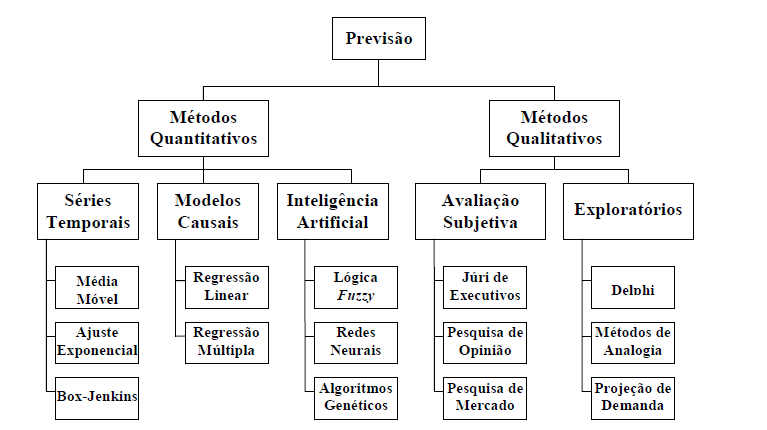
\includegraphics[width=0.90\textwidth]{./Figs/02-junior-metodos-previsao-demanda.png}
          	\caption{Métodos de previsão de demanda. Fonte: \cite{Junior2007}.}
          	\label{fig:metodosPrevisaoDemanda}}
          \end{figure}

E conforme a figura \ref{fig:metodosQuantitativos}, os métodos quantitativos se ramificam em 2 tipos, as séries temporais e os modelos causais.

          \begin{figure}[H]
          	\center{          		
            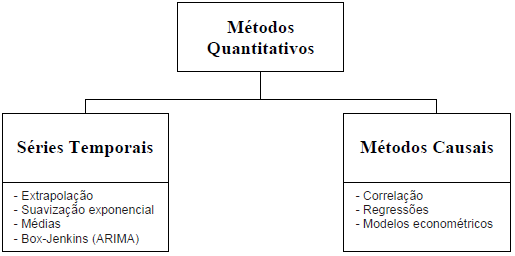
\includegraphics[width=0.90\textwidth]{./Figs/01-junior-metodos-quantitativos.png}
          	\caption{Tipos de métodos quantitativos. Fonte: \cite{Junior2007}}.
          	\label{fig:metodosQuantitativos}}
          \end{figure}

O comportamento dos dados deste trabalho, apesar de ter uma distribuição de datas em função do tempo se classificando em um modelo de série temporal, assume-se a hipótese que tem tal comportamento impactado por relações causais com outras variáveis como recesso acadêmico, feriados, eventos, precipitações intensas que causam trânsito local e impactam na logística e frequência do público, entre outras variáveis de causas menos aparentes

\section{Redes Neurais Artificiais}
%\TODO{o comando subcaption* nas figuras está acarretando na numeração incorreta. Veja o que fiz nas figuras anteriores e replique para as demais}

As redes neurais, ou redes neurais artificiais  para sermos mais precisos, representam uma tecnologia que tem raízes em muitas disciplinas: neurociência, matemática, estatística, física, ciência da computação e engenharia \cite{Haykin1994}. 
De modo geral as redes neurais fazem parte da grande área de conhecimento denominada Inteligência Artificial (IA), termo cunhado em 1956 por John McCarthy \cite{kaplan2019siri}.


"A inteligência artificial é o ramo da ciência da computação que se ocupa do comportamento inteligente." \cite{Luger2004}. Sistemas de inteligência artificial buscam então resolver funções e problemas que seres humanos conseguem resolver melhor do que máquinas convencionais, usando sua capacidade de abstração e aprendizagem com o erro. De uma forma geral, a IA pode ser dividida em diversas subcategorias, a descrição completa de todas as subcategorias está fora do escopo deste trabalho, que tem como foco o desenvolvimento da subcategoria de redes neurais artificiais, e dos modelos de perceptron de múltiplas camadas e das redes recorrentes GRU.

% "Um neurônio é uma unidade de processamento de informação que é fundamental para a operação de uma rede neural."\cite{Haykin1994} 

As redes neurais artificiais são formadas por neurônios artificiais interconectados que são capazes de processar múltiplos valores de entradas, e reagir produzido uma resposta relacionada à essas entradas. Como qualquer outro método de aprendizado de máquina, este modelo busca obter um aprendizado a partir dos dados de entrada recebidos, criando uma capacidade de generalização de problemas e assim buscam o objetivo principal de resolver novos problemas com este aprendizado.

Uma rede neural pode não produzir uma resposta esperada, resolvendo erroneamente um problema, assim como o cérebro humano tem limitações de aprendizado, que levam o homem a cometer falhas de decisões ou ações por um aprendizado mal treinado. Por isso as características fundamentais que tornam uma rede neural artificial em uma boa solução, é um bom planejamento de sua topologia, e método de treinamento, que serão explicados nas seções a seguir.

\TODO{QUILES - NA IMAGEM DO NEURONIO BIOLÓGICO ABAIXO EU TENHO UM PROBLEMA POIS TIREI O SUBCAPTION, MAS AO CITAR A FONTE URL DA IMAGEM DENTRO DO CAPTION O TITULO DELA ESTOURA A MARGEM NA PÁGINA DE INDICE DE FIGURAS, VOU TER Q PESQUISAR MELHOR COMO POSSO FAZER ISSO}

\TODOR{Remova a figura. Não há necessidade de inserir uma representação do neurônio biológico aqui. Não esqueça de remover as menções a essa figura (se houverem)}

    % \subsection{Neurônio Artificial - Origem}
    %   \paragraph*{Neurônio Biológico}
    %     O modelo de neurônio artificial surge com a busca da inteligência artificial de reproduzir o comportamento de aprendizado humano, desenvolvendo computacionalmente seu elemento biológico principal de aprendizagem: O neurônio biológico. 
    %     \begin{figure}[H]
    %       \center{
    %         \includegraphics[width=0.65\textwidth]
    %         {./Figs/05-neuronio.jpg}
          
    %       \caption{Neuronio Biológico, Fonte: \url{https://pt.khanacademy.org/science/biology/human-biology/\\neuron-nervous-system/v/anatomy-of-a-neuron.}}
    %       \label{fig:NeuronioBiológico}}
    %     \end{figure}
    
    \TODOR{Todos os parágrafos abaixo podem ser removidos. Não há necessidade de se falar de Neurociência, etc. Inicie diretamente no parágrafo do Neurônio MCP}
    
    % Um neurônio biológico (Figura \ref{fig:NeuronioBiológico}) trata as informações recebidas por meio de seus dendritos e processa-as em seu corpo celular, tal reação à esses estímulos recebidos gera um sinal de saída como resposta aos estímulos, enviado através do axônio. Esse estímulo é repassado como sinal de entrada, através de outros neurônios por meio de seus dendritos, e o ciclo se repete em uma vasta rede.
    % Controlando essas conexões, pontos de contato entre a resposta de um neurônio e a entrada de outro, existem as sinapses. Elas funcionam como agentes que permitem a interação acontecer ou inibem, e são acionadas por um conjunto somatório de estímulos. Se tal somatório de estímulos for satisfatório, elas permite a transmissão de sinal elétrico pelo axônio até o dendrito de um neurônio vizinho, formando um ciclo de aprendizado em uma rede neural biológica.
    
    % Fazendo um breve estudo sobre neurociência e analisando um trabalho analítico sobre a plasticidade cerebral, encontra-se o trabalho de \citeonline{Muhammad2014} que demonstra que a propriedade fundamental do cérebro é a sua capacidade de mudar com uma grande variedade de experiências, inclusive lesões que provocam perdas de neurônios, abordando princípios de plasticidade cerebral, e mostra também que a capacidade de aprendizado de mamíferos que sofreram uma redução de neurônios causada por lesões, pode ser restaurada não somente pela recuperação desses neurônios perdidos, mas sim por novas conexões e sinapses entre outros neurônios, evidenciando que durante a vida destes seres, sua topologia de conexão de neurônios cerebrais permanece em constante reajuste.
    
    % E também em um experimento recente realizado no artigo \citeonline{Fapesp192}, é evidenciado que o cérebro humano possui atualmente 86 bilhões de neurônios interconectados, e que sua capacidade de aprendizado e habilidades evolutivas também vêm aumentando em conjunto com seu número de neurônios e topologia de rede neural biológica, e que há 30 milhões de anos atrás nós homos sapiens, tínhamos apenas 2,5 bilhões de neurônios.
    
    %\paragraph*{Neuronio Artifical - MCP}
    Warren McCulloch e Walter Pitts em 1942 observando o neurônio biológico iniciam a busca de um modelo computacional do mesmo. McCuloch era psiquiatra e neuroanatomista e passou cerca de 20 anos refletindo e estudando sobre a representação do sistema nervoso, em 1942 ele convidou Pitts, que era matemático, para fazer parte das suas pesquisas. Em 1943 lançaram o artigo "A Logical Calculus of the Ideas Immanent in Nervous Activity." chegando em um modelo matemático do neurônio artificial. 
    
    \begin{figure}[H]
        \center{
          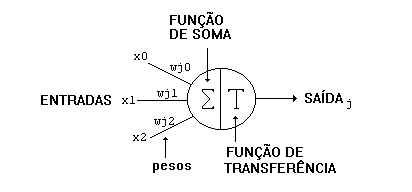
\includegraphics[width=0.65\textwidth]
          {./Figs/06-neuronio-artificial.png}
       
        \caption{Neuronio Artificial. Fonte: \url{http://redesneuraisartificiais.blogspot.com/2010/10/o-primeiro-modelo-de-um-neuronio-criado.html}} \label{fig:NeuronioArtificial} }
    \end{figure}
    
    Inspirado no neurônio biológico, o modelo de neurônio artificial da figura \ref{fig:NeuronioArtificial} proposto por McCulloch e Pits, denominado MCP, reage à um vetor de entradas $x_0$ à $x_2$ onde tem suas sinapses representadas por pesos numéricos $wj_0$ à $wj_2$, com uma soma ponderada dessas entradas que é controlada por uma função de transferência ou função de ativação, determinando se essa soma é maior que um valor numérico. Se essa soma for satisfatória o neurônio é ativado emitindo um valor de saída 1, caso contrário se emite um valor de saída 0.
    Todo o funcionamento deste modelo então é reduzido a responder se a soma recebida é maior que um valor numérico esperado. Contudo, associado a este neurônio não foi proposto uma forma automática para ajuste dos pesos, ou seja, não há um algoritmo de aprendizagem que possa treinar e tornar o neurônio viável para a solução de um problema \cite{Haykin1994}.
        
    \subsection{O Perceptron}

    O modelo de Warren McCulloch e Walter Pitts, apesar de conseguir simular o modelo de neurônio biológico e resolver algumas tarefas lógicas e matemáticas não atendia o objetivo principal da Inteligência Artificial: A capacidade de aprendizado.
    Para utilizar um modelo de neurônio artificial a fim da solução de um problema era necessário conhecer o ajuste dos pesos das entradas, e em uma tarefa de um cenário complexo e com muitas variáveis, ou pesos não perceptíveis ao valor esperado de saída, o ajuste não se torna trivial.
                
    Em 1958, o cientista da computação Frank Rosemblatt desenvolveu o primeiro modelo de rede neural artificial com um algoritmo de aprendizado para o neurônio MCP, denominada de Perceptron, para solucionar este problema de ajuste de pesos.
    Basicamente neste novo modelo, os pesos das conexões são ajustados de forma autônoma com a introdução de pessoas associados e um valor bias, a fim de buscar um reconhecimento autônomo de padrões. Tarefas de reconhecimento de padrões simples com separações lineares os seres humanos conseguem realizar de forma trivial mas ainda era um desafio para tal problema se resolvido por uma máquina.
                
    Então em 1969, Marvin Mjinsky e Seymour Papert realizaram uma publicação comprovando essa limitação de aprendizado à uma combinação linear, e provaram que o perceptron é limitado à resolução de problemas que são resolvidos ou classificados por apenas 1 linha, ou seja, problemas linearmente separáveis que consiste na mesma limitação do processo de regressão linear múltipla.
                
    Na figura \ref{fig:problemasLineares} o perceptron não pode solucionar o problema (b). E essa limitação desmotivou e parou os estudos com perceptrons.
      \begin{figure}[H]
      	\center{
      		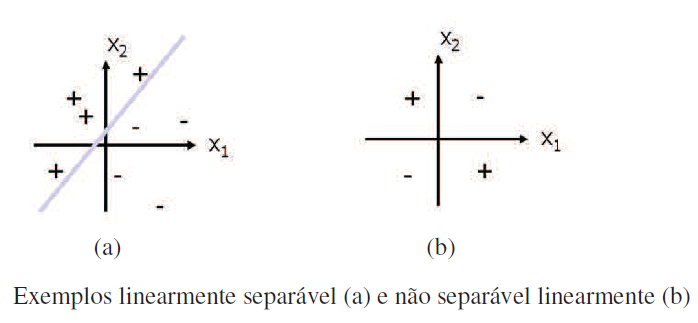
\includegraphics[width=0.65\textwidth]
      		{./Figs/10-limite-perceptron.png}
      
      	\caption{Problemas Linearmente Separáveis e Não Separáveis. Fonte: \cite{Flavia2014}.}\label{fig:problemasLineares}}	
      	
      \end{figure}
    
    Em 1986 James McClelland e David Rumelhart proporam o método de desenvolvimento de uma rede neural de perceptrons, tangendo mais ainda a inspiração da solução no cérebro humano. O processo resume o treinamento do perceptron simples aplicado à um conjunto de perceptrons interligados, e assim solucionando problemas complexos que podem ser resolvidos com uma combinação de soluções, e assim como na figura \ref{fig:doisPerceptrons}, uma rede de 2 perceptrons podem solucionar a separação dos conjuntos, combinando as soluções lineares de cada perceptron.
    
    \TODO{QUILES - A REGINA RECLAMOU QUE NA IMAGEM ABAIXO ESTÁ APARECENDO UM (b) MAS NÃO TEM (a) PORÉM ESSA IMAGEM É UMA ADAPTAÇÃO DA IMAGEM ANTERIOR... É A FIGURA (b) DA IMAGEM ANTERIOR COM A SOLUÇÃO MLP QUE FOI DESCOBERTA PELO JAMES MC. E DAVID RUM.}
    
    \TODOR{Refaça a figura e remova o (b). Idem para a figura anterior. Evite usar figuras externas ao seu trabalho. Essa figura é fácil de desenhar. Outra questão, você recortou a figura com o rótulo original "Exemplos linearmente..." e depois inseriu o seu próprio caption. Essa também foi uma reclamação da regina}
    
      \begin{figure}[H]
      	\center{
      		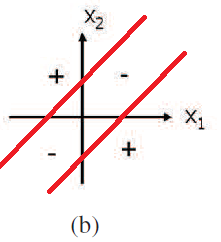
\includegraphics[width=0.30\textwidth]
      		{./Figs/11-solucao-mlp.png}
      	
      \caption{Problemas Linearmente Não Separáveis. Múltiplas Soluções.}  \label{fig:doisPerceptrons}}
       \end{figure}
    
    A rede perceptron , conforme demonstrado na literatura de \citeonline{Haykin1994}, possui apenas uma camada de entrada e saída, a saída utiliza como função de ativação a função degrau $ \delta(.) $ que define quando o neurônio emitirá o sinal lógico 1 ou quando emitirá o sinal lógico 0.
    
    O sinal de saída do perceptron entende-se então por:
    $y_k= \delta(\sum_{i=1}^{n}x_i W_{ki}+b_k)$
    \begin{itemize}
    	\item $ x_i $ - sinais de entrada do neurônio;
    	\item $ w_{ki} $ - pesos sinápticos do neurônio;
    	\item $ b_k $ - bias ou limiar de ativação;
    	\item $ \delta(.) $ - função de ativação;
    	\item $ y_k $ - sinal de saída do neurônio.
    \end{itemize}
    
    \begin{figure}[H]
    	\center{
      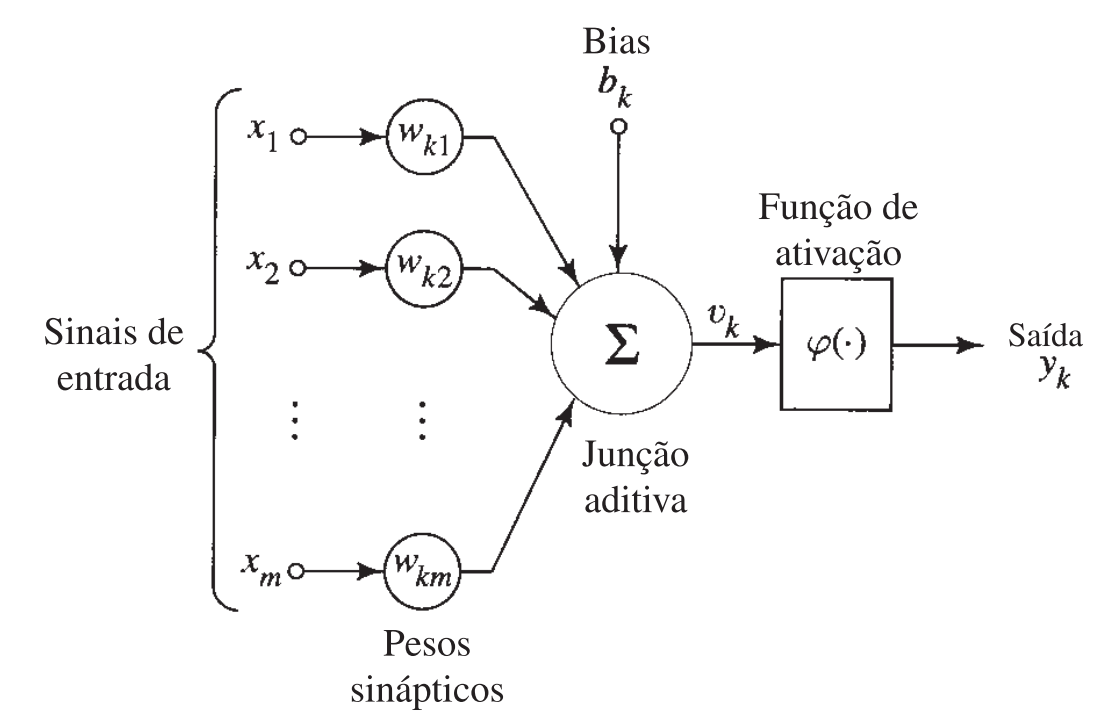
\includegraphics[width=0.65\textwidth]
      {./Figs/08-perceptron.png}
    
    \caption{Neurônio Artificial Perceptron. retirado de \citeonline{Haykin1994}} \label{fig:perceptron} }
    \end{figure}
    
     Em algumas literaturas o bias pode ser reduzido a um peso $W_0$ com entrada $X_0$ fixo em 1 no neurônio, a representação gráfica da topologia pode mudar, mas no somatório de saída, o calculo continua o mesmo.
    
     A função de ativação $\delta$ se apresenta de forma linear ou não linear, determinando a saída de um neurônio a partir do seu potencial de ativação, a figura \ref{fig:activation_functions} ilustra as funções de ativação mais utilizadas nos conceitos e experimentos realizados na literatura de \cite{MCAI}.
    
     \begin{figure}[H]
    \center{
    	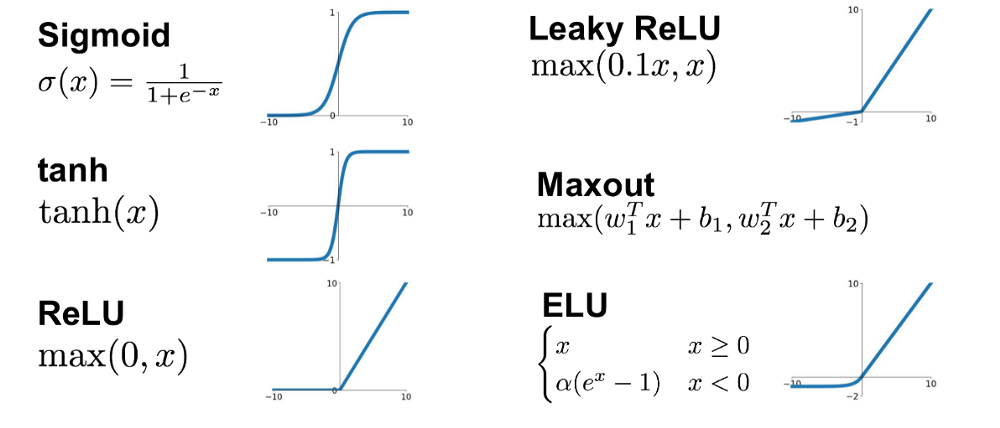
\includegraphics[width=0.80\textwidth] {./Figuras/mc_ai/activation_functions.png}
    
    \caption{Funções de Ativação Fonte: \cite{MCAI}}} \label{fig:activation_functions}
    \end{figure}
    
     A função de ativação dá a capacidade do perceptron. quando conectado em rede, de resolver problemas lineares e não lineares, agregando adaptação e improviso ao resolver programas que não estão contidos em seus dados de alimentação.
     
     Nos parâmetros de previsão de consumo no ICT Unifesp, a função ReLu ganha destaque para utilização em neurônios nas camadas ocultas da rede neural, por ser simples e eficiente para a aplicação nos experimentos, visto que na fase feed-forward tem efeito parecido com a função identidade, e na fase feed-backward durante o reajuste dos pesos pelo otimizador, conforme ilustrado na figura \ref{fig:ReLu}, sua derivada produz efeito degrau zerando valores negativos e sendo adequada na aplicação do domínio destes parâmetros, visto que todas as variáveis endógenas e exógenas utilizadas como parâmetros de predição, como por exemplo pressão atmosférica, vendas e consumo de dias anteriores, datas, entre outros, não possuem valores negativos. Já a função linear ganha destaque para aplicação no neurônio de saída que determina o consumo previsto para uma data no futuro, pois na fase feed-backward do reajuste dos pesos pelo algoritmo de treino backpropagation, a derivada da função linear se torna zero, fazendo com que o algoritmo de treino transforme apenas os pesos sinápticos dos parâmetros de entrada os pesos sinápticos dos neurônios nas camadas ocultas da rede, sem interferir no neurônio de saída.
     
      \begin{figure}[H]
    \center{
    	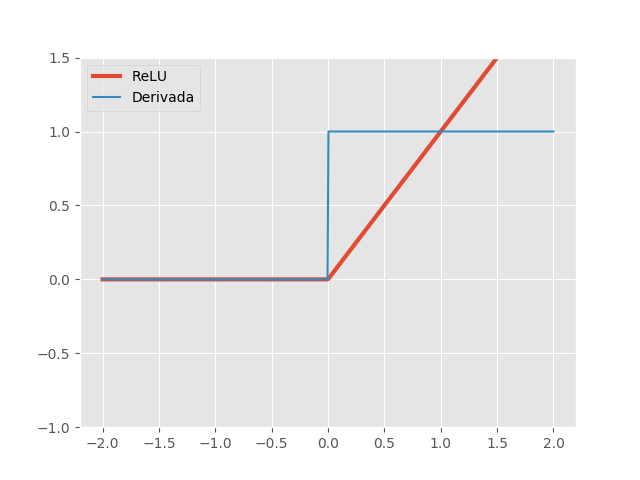
\includegraphics[width=\textwidth] {./Figuras/RELU.png}
    
    \caption{Derivada da função ReLu} 
    } \label{fig:ReLu}
    \end{figure}
    			
    		  %\paragraph*{Perceptron - Treino Supervisionado}
    \cite{Almeida2013} cita em sua análise que o processo de aprendizado do perceptron pode ocorrer de forma supervisionada quando o neurônio deve aprender a relacionar um conjunto observado de variáveis à um valor observado de saída deste mesmo conjunto. O neurônio recebe os sinais de entrada $Xi$ e produz uma saída $Yi$ através do combinador linear e função $\delta$ de ativação; compara essa saída $Yi$ com a observação $i$ obtida do conjunto de dados (ponto chave do processo de treino supervisionado) e por fim essa comparação irá gerar um erro $e$.
                
                % \subparagraph*{Critério de parada}
    De acordo com algum critério adotado em cada contexto de aplicação do perceptron, este erro pode ser aceitado e o neurônio mantém o valor de seus pesos $Wi$ que impactam na saída $Yi$ desejada. A aprendizagem do neurônio também pode atingir um critério de parada após N épocas de treinamento, diversos critérios de paradas  podem ser combinados.  
                	
                % \subparagraph*{Época de treinamento}
    Se o critério de parada não for aprovado, uma nova época de treinamento (ou repetição de interação) é iniciada mesmos valores $X_i$ e $Y_i$ passados, os valores de pesos $Wi$ são reajustados com a taxa de aprendizagem, buscando o objetivo de se obter um erro menor.
                	
                % \subparagraph {Taxa de aprendizagem}
    Esse reajuste de pesos $Wi$ denomina-se taxa de aprendizagem, $\alpha$ que pode ter valores de escolha livre ao contexto de aplicação do perceptron, para reajustar estes pesos $Wi$. Assim que a taxa de aprendizagem ajusta os pesos, uma nova época N+1 de treinamento está se iniciando buscando novamente um erro menor. Ressaltando então que o critério de parada pode ser acionado e interromper o reinicio do processo, se for estipulado um limite para o valor de N combinado ou não com um limite para o erro. 
            	
  	    %%%%%%%%%%%%%%%%%%%%%%%%%%%%%%%%%%%%%%%%%%%%%%%%%%%%%   
    \subsection{Rede Perceptrons Múltiplas Camadas - MLP}

    A solução base para se combinar 2 ou mais camadas de perceptrons a fim de se resolver um problema com a combinação de 2 ou mais soluções lineares, é a utilização de um perceptron combinador de sinal de saída, já que cada perceptron pode ter múltiplas entradas e somente uma saída. Dessa forma as redes neurais vão formando colunas de perceptrons interconectados. Cada coluna é denominada uma camada oculta da rede neural. A ultima camada deve ter o número de perceptrons correspondente ao número de saídas desejadas. Na figura \ref{fig:MLP} encontra-se uma rede neural com 2 camadas ocultas e a camada de saída possui 3 neurônios que emitem 3 sinais distintos de saídas.
    
    \begin{figure}[H]
     \center{
     	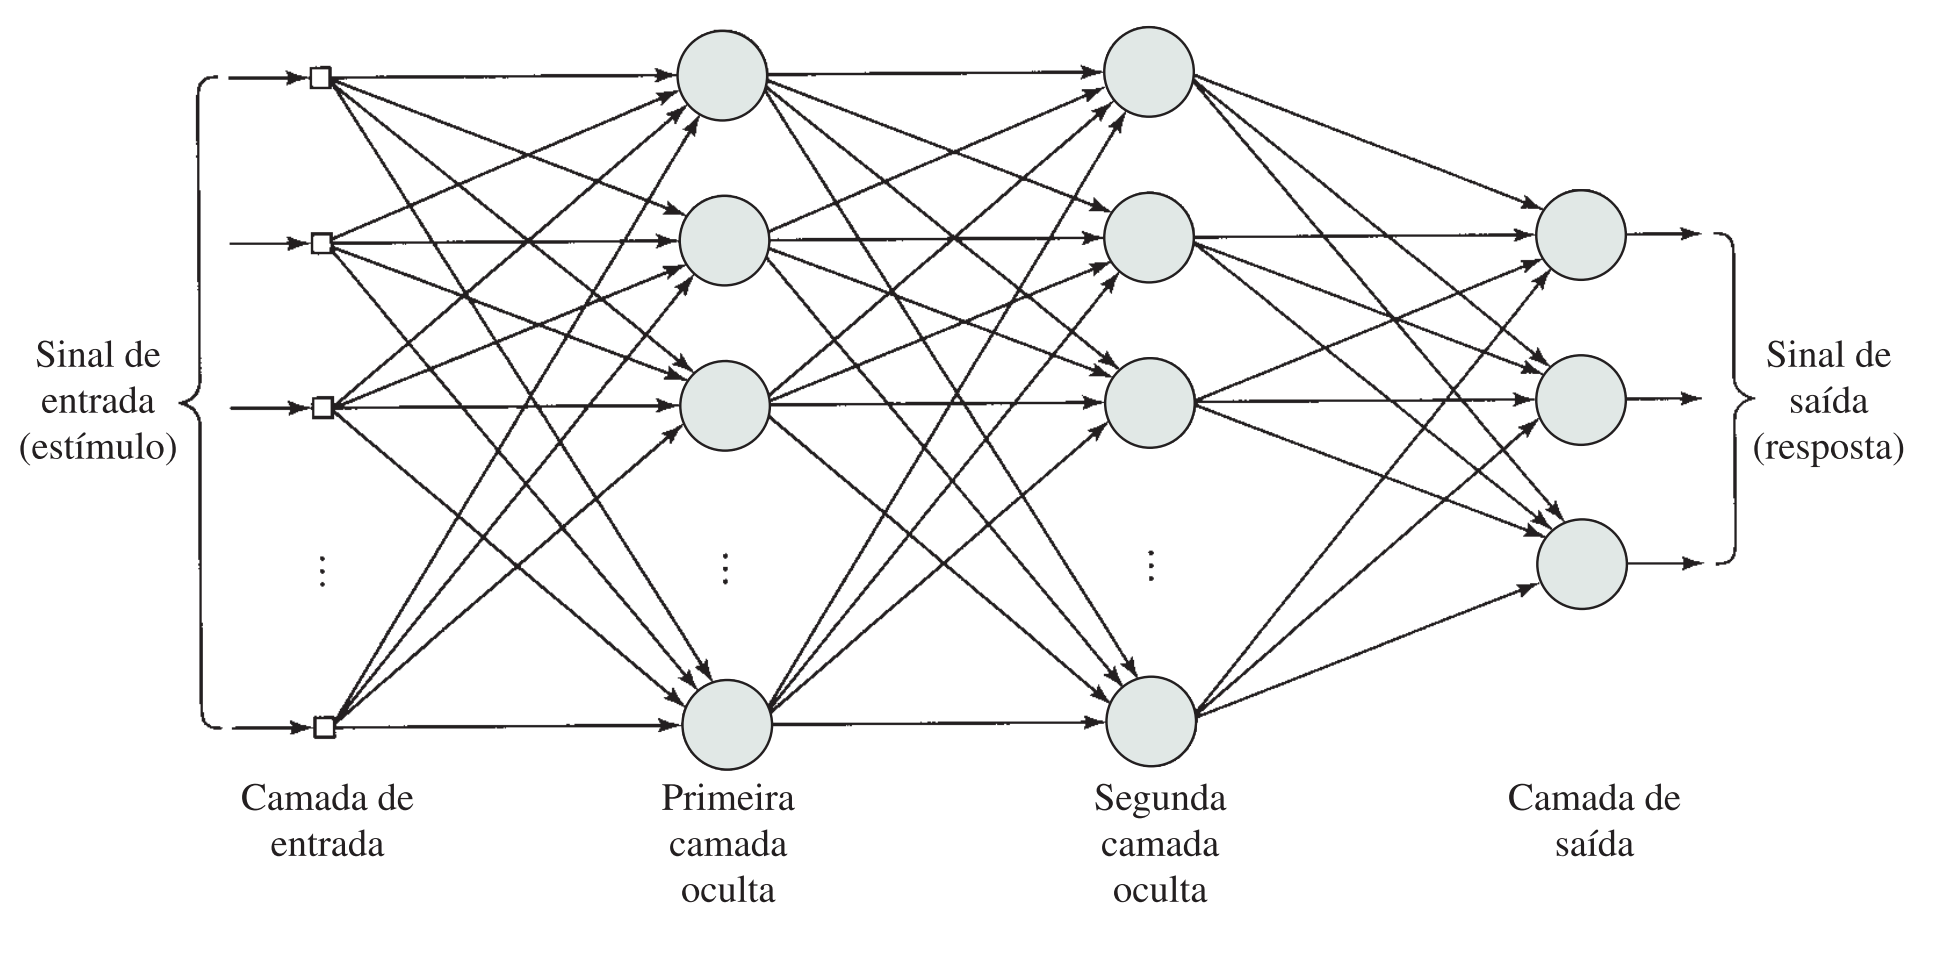
\includegraphics[width=0.65\textwidth]
     	{./Figuras/haykins_rede_MLP.PNG}
     
     \caption{Rede de perceptrons com múltiplas camadas, Fonte: \cite{Haykin1994}\label{fig:MLP}
     }}
    \end{figure}
    
    Nesta rede denominada MLP (Multilayer Perceptron) a camada de entrada é representada por uma coluna de ícones quadrados na figura \ref{fig:MLP} , que representam os parâmetros do problema a ser analisado, e tais parâmetros passam pelas transformações e cálculos realizados pela rede neural gerando as soluções do problema a ser resolvido, como sinais de saída.
    
    Na primeira camada oculta os neurônios possuem geralmente uma função de ativação, e conceitualmente no mínimo 1 neurônio desta primeira camada oculta deve receber no mínimo 2 parâmetros de entrada.
 
% \paragraph*{Treino e Validação da MLP}
    O conjunto de dados de entrada na rede MLP, do tipo supervisionada, deve ser dividido em 2 partes principais, Treinamento e Validação. É importante salientar que as observações de ambos os conjuntos devem originar do mesmo conjunto de dados para representar o mesmo problema.
    
    O conjunto de dados da validação e treino somados devem formar exatamente o conjunto original, sem informações excedentes ou em falta.
    
    Os dados de treino e dados de validação podem ser separados com diversas heurísticas inerentes aos temas de cada problema, na literatura de \cite{DLB} são encontradas por exemplo heurísticas de separação de conjuntos em ordem aleatória com 70\% dos dados para treino e 30\% dos dados para validação, sendo os dados de treino os responsáveis pelos reajustes de pesos e capacidade de generalização da rede, e os dados de validação responsáveis pelo processo de validação pós-treino.
    
    É importante adotar um bom critério de parada de treino, pois um treino prolongado tende a convergir em ajustes de pesos memorizados dos valores observados nos dados de treino e isso causa o fenômeno de overfitting na rede neural, que é a perda da capacidade de generalização. Pesos sinápticos que sofrem processo prolongado de reajustes acaba "viciando" a rede neural para reconhecer apenas os dados de treino.
    
    % 	\subparagraph{ Parada do erro mínimo:}
    O critério de parada do erro mínimo encerra o treinamento da RNA quando a mesma obtém um erro menor que o mínimo estipulado para o valor observado, este é o critério mais simples, adotado nos casos onde existe um limiar de erro já determinado pelo problema, entre o valor observado e o valor a se predizer.
    
    % 	\subparagraph{Parada por número de épocas:}
    Um critério de parada pode ser limitado também ao número de épocas de treino. A determinação  deste número de épocas pode ocorrer por tentativa e erro, visto que haverá a convergência de um número pequeno para uma baixa capacidade de aprendizado, e a convergência de um número grande para o processo de overfitting. Logo é necessário realizar experimentos que validem número de épocas fora desses intervalos de convergência.
    
    % 	\subparagraph{Parada por validação cruzada:}
    Por fim a validação cruzada é a técnica que se utiliza os dados dos conjuntos de validação e treino de forma cruzada, neste processo então, os dados de treino são utilizados no processo interativo de aprendizagem, e no fim deste processo o conjunto é validado com os dados de validação, obtendo-se um novo erro de validação.
    A medição do erro de validação passa por um processo de avaliação em função do número de épocas, a fim de se detectar um ponto de número de épocas onde o erro quadrático médio da amostra de validação sofre uma curva de crescimento após um limiar de decréscimo.
    
    É notório observar que o erro quadrático médio das amostras de treinamento sofrerá um decréscimo em função do aumento do número de épocas de treinamento, convergindo ao processo de overfitting, ou memorização da rede.
    
    O ponto de parada no limite inferior do erro quadrático médio da amostra de validação, será o ponto ótimo de parada de treinamento.
    
    \begin{figure}[H]
      \center{
      	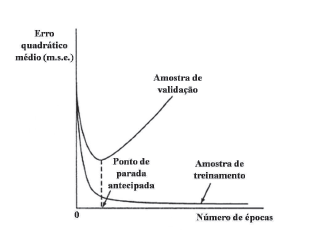
\includegraphics[width=0.5\textwidth]
      	{./Figs/14-validacaocruzada.png}
      
      \caption{Ponto ótimo de parada da validação cruzada, Retirado de \cite{Flavia2014}} \label{fig:validacaoCruzada}} 
    \end{figure}

    \subsection{O Algoritmo de Retro Propagação \textit{Backpropagation}}

    A rede Perceptron Múltiplas Camadas com Retro Propagação de Erro (do inglês, M.L.P Backpropagation), faz o reajuste dos pesos sinápticos dos neurônios através de duas fases:
     \paragraph*{Feed-forward} Nesta primeira fase de treino os sinais $X_{i0},X_{i0},...,X_{in}$ com sua respectiva saída $Y_i$ do conjunto de dados são apresentados à todos os neurônios da primeira camada. O processo de propagação do sinal de saída de cada neurônio segue o princípio do neurônio artificial apresentado na seção anterior, que envia o sinal de saída como um sinal de entrada ao neurônio seguinte.
     
     \paragraph*{Feed-backward} Nesta fase é obtido um valor de erro da camada de saída. Este erro é utilizado na equação de reajuste do peso sináptico das conexões dos neurônios da camada de saída com o sinal de saída dos neurônios da última camada oculta. E depois este erro é propagado realizando outra equação de reajuste de peso sináptico das conexões dos neurônios nas camadas anteriores, no sentido contrário em direção à camada de entrada. Isto permite que os pesos sináptico de todas as camadas de intermediárias neste processo tenham seus pesos ajustados.
     
     \begin{figure}[H]
     	\center{
     		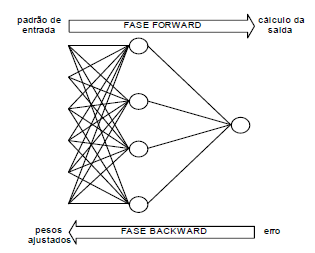
\includegraphics[width=0.65\textwidth]
     		{./Figs/13-mlp-back.png}
     	
     	\caption{Fases de treino da MLP-Back-Propagation.} \subcaption{Fonte:  \cite{Almeida2013}}\label{fig:MLP2}}
     \end{figure}
     
     \paragraph*{MLP Backpropagation em R.U em trabalhos relacionados}
     De acordo com o trabalho de \cite{Lopes2008}, a rede neural perceptron de múltiplas camadas é utilizada para tratar a previsão de demanda do R.U da UFV, utilizando apenas como variáveis quantitativas as 5 ultimas observações anteriores ao dia a se analisar, e como variáveis qualitativas o dia da semana variando de segunda a sexta, em valores binários.
     
    \begin{figure}[H]
      \center{
      	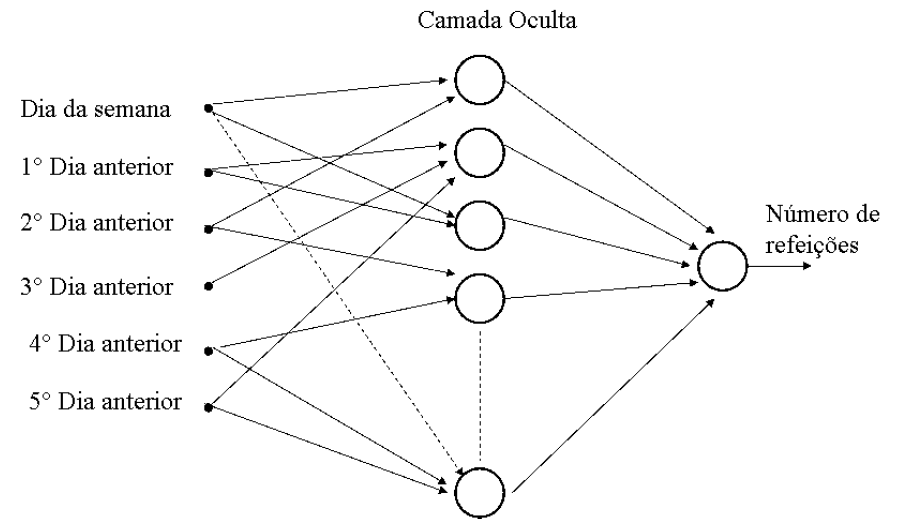
\includegraphics[width=0.65\textwidth]
      	{./Figs/15-rna-lopes.png}
      
      \caption{Rede Neural Perceptron de Múltiplas Camadas. Fonte:\cite{Lopes2008}.}\label{fig:mlp-lopes}}
    \end{figure}
    
    Conforme  o trabalho realizado por \citeonline{Rocha2011} com neurônios artificiais para prever a demanda do R.U da UNESP, envolve apenas uma única camada de entrada e uma segunda camada para saída, porém com uma diversidade maior de variáveis de entrada correlacionadas com o consumo do restaurante. 
    \begin{figure}[H]
      \center{
      	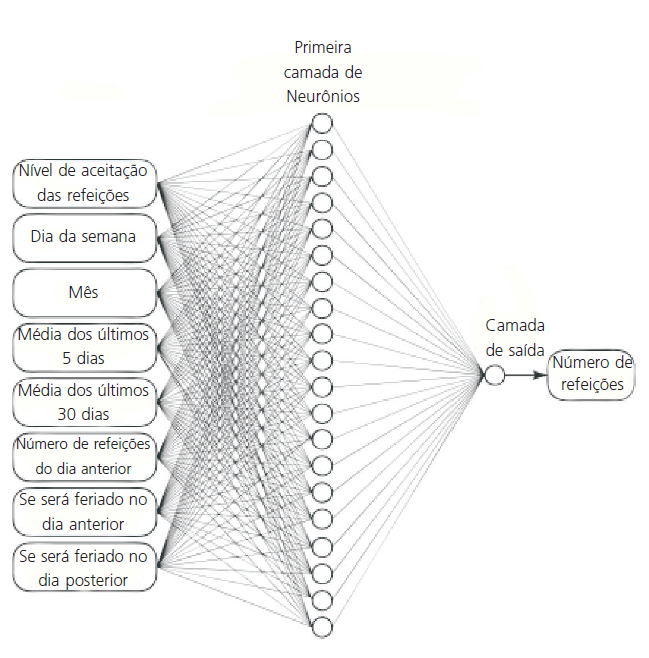
\includegraphics[width=0.65\textwidth]
      	{./Figs/16-rna-rocha.png}
      
      \caption{Rede Neural Perceptron de Múltiplas Camadas. Fonte: \cite{Rocha2011}} \label{fig:rnaRocha}}
    \end{figure}
    
    Ambos os modelos possuem topologia de uma camada oculta para entrada dos dados, e uma camada de saída. que de acordo com  a análise de \citeonline{Braga2000}  é citado que através de uma análise de Cybenko, uma camada intermediária é o suficiente para aproximar qualquer função contínua e 2 camadas intermediárias são suficientes para aproximar qualquer função matemática, e devendo ser observado o fato de que em alguns casos, a utilização de 2 ou mais camadas pode facilitar o treinamento da rede, porém a utilização de um grande número de camadas intermediárias ou ocultas, é inviável, pois em cada uma delas a estimativa do erro se trata de uma estimativa da estimativa do erro da camada anterior, e este cascateamento de estimativas pode se tornar menos preciso à medida que cresce.
    
    Em conformidade com o trabalho de  \citeonline{Flavia2014}, o número de neurônios na primeira camada oculta é proporcional à dimensão do espaço de observação. Logo em modelos preditivos de demanda, supracitados, observa-se que no mínimo, na primeira camada oculta, é utilizado um número de neurônios igual ao número de variáveis que influenciam no dado preditivo.
    
    \paragraph*{Parâmetros de treino da MLP Backpropagation}
    A definição da função $\delta$ de ativação interfere na linearidade  do modelo a ser analisado, sendo a função sigmoide a mais popular na literatura. 
    
    A taxa de aprendizagem, define a velocidade de reajuste dos pesos, podendo variar de 0 a 1. Ressalta-se que uma taxa próxima de 1 provoca picos oscilatórios na taxa de aprendizado, e taxa próxima de 0 provoca lentidão da convergência de aprendizagem. Valores comuns de utilização ficam entre 0,2 e 0,8.
    
    % \subsection{Treino da MLP - BackPropagation para 1 sinal de saída}
    No caso do problema de predição de demanda onde se busca apenas um valor de saída, que é a previsão de vendas em relação às variáveis de entrada, o cálculo de reajuste dos pesos da camada de saída é reduzido à apenas 1 neurônio na camada de saída.
    
    O treino da rede perceptron com backpropagation obtém o sinal de saída no último neurônio $s$ da rede, através da propagação dos sinais de saída dos neurônios anteriores da rede, feito pela aplicação da combinação linear dos sinais de entrada com os pesos sinápticos em uma função de ativação. É calculado o erro quadrático deste sinal de saída e a regra do Gradiente Descendente com base neste erro é utilizada para o reajuste dos pesos sinápticos em todas as conexões de todos os neurônios. O processo é denominado regra delta generalizada, $\Delta$
    
    O principal objetivo de todo o método backpropagation conforme o avanço de épocas, é o treino em uma determinada época reduzir a média de erros quadráticos do conjunto de validação ( $m.s.e$ ) em $n$ iterações de validação desta época:\\
    $m.s.e = \frac{1}{n} \sum_{k=1}^{n}e(k)$
    É importante observar que 1 época consiste no par treino e validação. Logo após o treino, os erros $e(k)$ serão obtidos novamente através das entradas $Y_i$ do conjunto de validação, e respostas propagadas $Y_\mu$ na camada de saída da rede já treinada, para então o $m.s.e$ ser calculado.
    
    O valor $m.s.e$ será o critério de parada do treinamento de toda a rede e deve ser observado a cada época de treinamento, assim que este valor atingir um ponto ótimo, conforme figura \ref{fig:validacaoCruzada} deste ponto ótimo o critério de parada será verdadeiro e o treinamento deve parar, pois a partir desse ponto a rede converge à um overfitting (divergindo de uma capacidade de generalização, e memorizando os dados de treino, podendo ter sua estimativa eficiente somente no conjunto de dados de treino).
    
    Ressaltando que toda saída de todo neurônio $j$ da rede, com $n$ entradas, é calculada através da equação:\\
    $ Y_{\mu}(j) = F(\mu)$\\
    Onde $\mu = (\sum_{i=1}^{n} (Xi_{n}(j)*Wi_{n}(j) + b)$ é o potencial de ativação do neurônio $j$ e $F$ é a função de ativação do neurônio.
    
    %%%%%%%%%%%%%%%%%%%%%%%%%%%%%%%%%% 
    \paragraph*{Fase Feedforward}
    Nesta fase, em determinada época $(k)$, em um vetor de $n$ variáveis $Xi$ correspondentes à um total de venda $Yi$, todos os neurônios $j$ propagam o sinal de saída através do calculo de $Yi_{\mu}(j) = F(\mu(j))$. No cálculo de $\mu$ os pesos sinápticos de cada neurônio $j$ conectado à uma entrada $Xi_{n}(j)$ são $Wi_{n}(j)$. A saída estimada pela rede será $Yi_{\mu}(s)$.
    
    Se a iteração $i$ da época $k$ for a primeira, todos os pesos $Wi_{n}j$ em todos os neurônios, são inicializados com valores aleatórios pequenos.\\ 
    
    O valor de $Yi_{\mu}(j)$. dos neurônios da primeira camada oculta, são obtidos de forma que $Xi_{n}(j)$ são os sinais de entrada das variáveis de 1 à $n$.
    
    O valor de $Yi_{\mu}(j)$. dos neurônios das próximas camadas, inclusive a de saída, utiliza o sinal de saída $Yi_{\mu}$ dos neurônios da camada anterior conectados à $j$ como um sinal de entrada $Xi_{n}$.
    
    %%%%%%%%%%%%%%%%%%%%%%%%%%%%%%
    \paragraph*{Fase Feedbackward}
    O Processo de reajuste dos pesos sinápticos com o objetivo de atingir a minimização do erro quadrático da validação, é feito pelo método do Gradiente Descendente, reajustando os pesos sinápticos $Wi_{n}(j)$ correspondente à cada neurônio $j$ da rede, para um valor $\Delta Wi_{n}(j)$, da seguinte forma:\\
    $\Delta Wi_{n}(j) = \eta*\delta_j*Xi_{n}(j)$\\
    
    \subparagraph*{Regra $\delta$ para neurônio de saída}
    Exclusivamente para a camada de saída, $\delta$ é calculado por\\
    $\delta_s = (Yi - Yi_{\mu}(s) )*F'(\mu(s))$.
    
    O valor dos $n$ pesos $Wi_{n}(s)$ do neurônio de saída $s$ com $n$ entradas vindas das saídas de neurônios $j$ das camadas anteriores, é obtido por $\Delta Wi_{n}(s) = \eta*\delta_s*Yi_{\mu}(j)$\\.
    
    %%%%%%%%%%%%%%%%%%%%%%%%%%%%%%%%%%%%%%%%%%%%%%%%%%%%%%%%%%%%%%%%
    \subparagraph*{Regra $\delta$ para neurônios de camadas ocultas}
    Nesta etapa, os neurônios $n$ da camada oculta obterão seu $\delta$ através da seguinte equação usando o $\delta$ dos $m$ neurônios da camada posterior que se conectam à ele:\\ 
    
    $\delta_n = F'(\mu(n))*(\sum \delta_m*Wi_{n}m)$\\
    
    Na rede neural de 1 camada oculta e 1 neurônio de saída, a soma será reduzida à apenas 1 neurônio, ficando então a regra $\delta$ da seguinte forma:\\
    
    $\delta_n = F'(\mu(n))*(\delta_s*Wi_{n}s)$\\
    
    Por fim os pesos das $n$ entradas $Wi_{n}(n)$ conectadas ao neurônio $n$ terão seus pesos reajustados para a próxima iteração da seguinte forma:\\
    $\Delta W(i+1)_{n}(n) = \eta*\delta_n*Xi_{n}(n)$\\
    
    Após o reajuste chegar na primeira camada oculta, um novo vetor de observações $i$ é apresentado à rede repetindo, iniciando novamente a fase feed-forward e repetindo o ciclo até o fim das entradas.
    
    \subparagraph{Otimizador de reajuste dos pesos}
    
    Existem algoritmos populares que otimizam a convergência do reajuste dos pesos no treino de backpropagation. ganhando destaque o otimizador ADAM. A vantagem deste otimizador é a fusão das melhores características de 2 otimizadores o Momentum e RMSProp. Momentum acelera o reajuste dos pesos em busca dos erros globais mínimos, e RMSProp impede a busca na direção das oscilações.\newline
    Adam ou Adaptive Moment otimization combina estas 2 heurísticas. O coeficiente de aprendizado, ou conhecido como "learning rate", popular para este processo de otimização tem valor definido por uma constante alpha, de valor escalar 0.001.
    Esta constante tem produzido resultados positivos em problemas de forecast (predições) de acordo com o popular ebook Machine Learning Mastery fundamentado pelo \citeonline{MLM}. Na Figura \ref{fig:otimizadores} o eixo y "Training cost" demonstra que quanto menor o custo de treinamento, maior a velocidade de convergência ao reajuste ideal dos pesos, e neste caso é notório a vantagem do otimizador Adam sobre os demais à medida do avanço no número de iterações.
    
    \begin{figure}[H]
    \center{
    	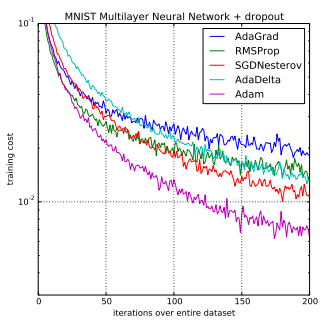
\includegraphics[width=0.80\textwidth]
    	{./Figuras/MLM/optimizers.png}
    
    \caption{Comparison of Adam to Other Optimization Algorithms Training a Multilayer Perceptron Fonte : \cite{MLM} }} 
    \label{fig:otimizadores}
    \end{figure}
    
    \subparagraph{Validação de treino}
        Após se encerrar uma época, que percorreu todas as i-ésimas entradas do conjunto de treino, um conjunto de dados de validação, previamente separado, é apresentado à rede.
        A validação ocorre só com a fase feedforward, obtendo-se os erros quadráticos da camada de saída com o dado de validação observado.
        Então é calculado o $m.s.e$, obtendo-se a média de todos os i-ésimos erros quadráticos do conjunto de validação.
        O valor $m.s.e$ deve ser acompanhado até que se atinja um ponto ótimo, ou seja, um limite inferior após k épocas.
        Quando este limite for atingido em uma época $k_o$, todos os parâmetros da rede dentro da época $k_o$ serão os parâmetros desejados do modelo final da rede.
        
        Quando a curva do $m.s.e$ estiver sendo realizada, não se saberá o ponto ótimo de parada, até que ele comece a ser superado, logo é importante arbitrar um número $l$ para salvar os parâmetros das $l$ épocas anteriores, em busca do ponto ótimo de parada, conforme figura \ref{fig:validacaoCruzada}
        
    \subsection{Redes Recorrentes: Células GRU}
    \TODO{QUILES - ESTÁ CORRETA ESSA FUNDAMENTAÇÃO SOBRE O MODELO GRU E PRECISO ESTENDER MAIS ?}

\TODOR{Colocar os termos em inglês em itálico. A ideia está ok, mas o texto está bem ruim. Precisa ser reescrito. Há erros de portugues e as frases estão confusas. Por exemplo, o que você quer dizer com ``pois utilizam elementos que decidem \textbf{o valores} de saída das unidades''?}

De acordo com  o livro Deep Learning Book escrito pela  \citeonline{DLB}, no capítulo de arquitetura de redes gated recurrent unit (GRU), as redes recorrentes GRU são uma simplificação das redes LSTM (Long Short Term Memory) que também  é uma melhoria das redes recorrentes clássicas encontradas na literatura, pois utilizam elementos que decidem o valores de saída das unidades, e que podem memorizar informações de entrada dadas por um grande intervalo de tempo, sem sofrer dissipação destes valores (resolvendo um problema clássico de memória de curto prazo em redes recorrentes), estes elementos de decisão e memorização dos valores dos gradientes de reajustes dos pesos são ilustrados como "reset gate" e "update gate" na figura \ref{fig:gru-arch}. Portanto este modelo, especificamente o GRU, foi viável na aplicação deste trabalho para a memorização da sazonalidade semestral e anual dos dados do restaurante universitário.
     	
        \begin{figure}[H]
        	\center{
        		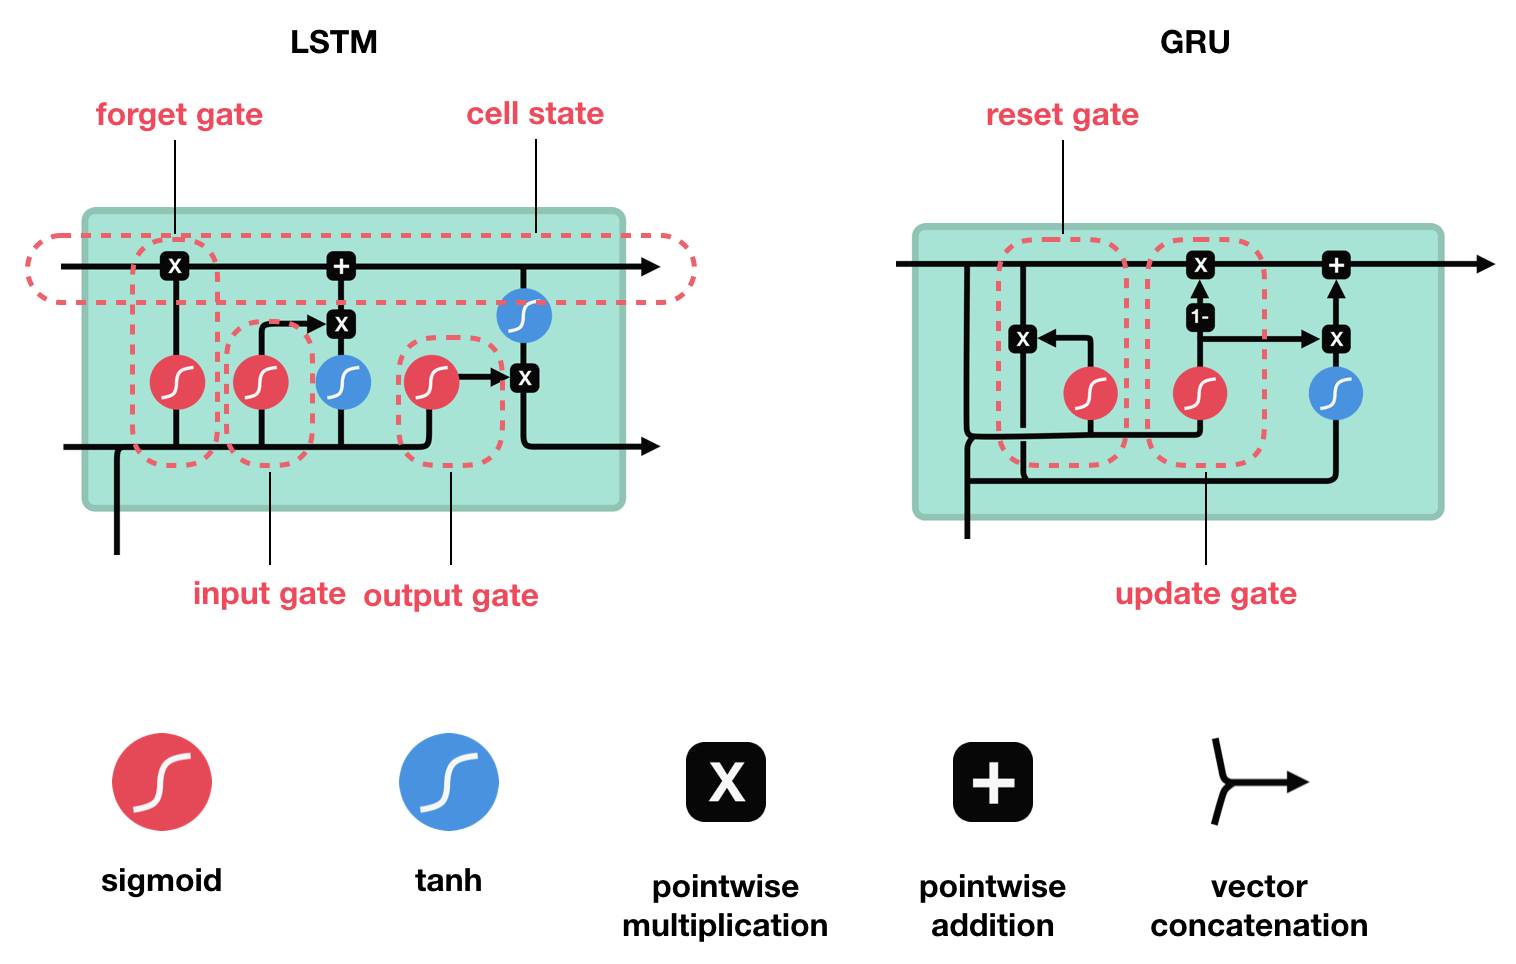
\includegraphics[width=0.80\textwidth]
        		{./Figuras/rnns.png}
        	
        	\caption{Arquitetura do modelo GRU, Fonte: \cite{DLB}} \label{fig:gru-arch}}
        \end{figure}
\chapter{Trabalhos relacionados} \label{cap:literatura}
  
    Este capítulo descreve os principais trabalhos relacionados encontrados na literatura referenciada neste trabalho.
    A seção de Revisão literária para previsão de demanda, cita a primeira referência literária encontrada na execução deste trabalho.
    A seção de previsão de demanda em outros ambientes cita o maior volume de referências encontradas durantes as pesquisas de predição de demanda, e a seção de Previsão de demanda em restaurantes universitários cita especificamente os estudos relacionados com uma parte dos métodos executados neste trabalho que são os modelos de redes neurais MLP, já o diferencial deste trabalho em relação à todos os trabalhos referenciados é a inclusão de redes neurais recorrentes modernas, denominadas GRU, fundamentadas no capítulo anterior, na seção de Inteligência Artificial, subseção Redes Recorrentes GRU.
    
    \section{Previsão de demanda em restaurantes universitários}
         No estudo estatístico feito por \cite{Landim2016}, foi analisada a correlação entre a temperatura e o consumo de refeições nos dias de vendas do restaurante universitário do campus ICT da Unifesp, sendo que os dados continham apenas uma pequena amostra das vendas do segundo semestre de 2016. Devido ao baixo volume de ocorrências, os dados foram submetidos à reamostragem via bootstrap. De acordo com os gráficos das amostras, identificou-se que a correlação mostrada nos gráficos da primeira metade do semestre e do período total do semestre formaram distribuições bimodais. Porém, na segunda metade do semestre formou-se uma distribuição unimodal. Portanto, concluiu-se que outras variáveis e outros modelos de análises deveriam ser utilizados para esta previsão de demanda.
        
         \cite{Lopes2008} faz o mesmo estudo deste cenário do ICT UNIFESP aplicado na Universidade Federal de Viçosa (UFV). Neste estudo, os dados utilizados foram somente o histórico de vendas do restaurante universitário, e nenhuma variável de ambiente foi coletada como temperatura, precipitação, número de alunos matriculados, etc. O algoritmo utilizado foi o Traincgp (Conjugate gradient backpropagation with Polak-Ribiere updates) no software Matlab. Este algoritmo não envolve o cálculo das derivadas segundas das variáveis e converge ao mínimo da função quadrática em um número finito de iterações como cita o autor. Foram então considerados para cada nó da rede neural, o dia da semana (como segunda, terça, quarta, quinta e sexta) e cada camada dessa rede utilizando os 5 dias anteriores para cada nó (as 5 segundas anteriores, 5 terças anteriores e assim sucessivamente) e, por fim, obtido um modelo pela rede que apresentou erro máximo de 3.
        
         \cite{Rocha2011} também realiza o estudo de demanda no restaurante universitário da Universidade Estadual Paulista Júlio de Mesquita Filho (UNESP), novamente com os métodos de redes neurais artificiais com backpropagation e utilizando apenas como fonte de dados (o histórico numérico das vendas realizadas), e outras variáveis intermediárias obtidas a partir deste, como médias de subconjunto de observações (médias de segundas-feiras). A única variável de ambiente coletada foi o número de feriados próximos à observação de venda. No estudo do total de dias analisados, verifica-se que em 73\% (187 dias), o método de média simples propiciou um maior erro em relação à RNA, que por sua vez ocasionou um erro maior nos 23\% (69 dias) restantes.Em se tratando de menor desperdício, observa-se que a RNA apresenta erros maiores que 50 refeições em 13 dias, enquanto o método da média simples apresenta erros maiores que 50 refeições em 58 dias, concluindo-se então que o método de RNA foi bem mais eficiente do que o cálculo de média simples utilizado pela administração do restaurante universitário.
      
      \section{Previsão de demanda em outros ambientes}
         \cite{RUAS2012} faz uma análise de previsão de demanda de energia elétrica no estado do Paraná, entre os anos de 2004 e 2006, utilizando redes neurais artificiais e máquinas de vetores de suporte. Apesar de não ser o mesmo exemplo do cenário do restaurante universitário do ICT UNIFESP, temos a distribuição dos dados de consumo coletados como uma série temporal. Nesta pesquisa de previsão de demanda de energia elétrica foi utilizada uma rede parcialmente recorrente de Elman, que permite a previsão de um passo de tempo à frente. Para que seja possível realizar a previsão para vários pontos à frente, é necessário utilizar os valores já previstos, ou seja, a saída da rede, como entradas da mesma.
        
         \cite{Almeida2013} analisa um cenário semelhante de demanda de energia elétrica, porém utilizando-se técnicas de previsão de demanda com Rede Neural Artificial do tipo Multilayer Perceptron combinado com lógica fuzzy que permite colocar variáveis de temperatura (entre outras) em um conjunto de regras que impactam no problema.
        
       \cite{Silva2010} também aplica técnicas de redes neurais para previsão de demanda de energia elétrica, com o estudo de variáveis climáticas, porém através de um modelo de MAPA SOM - (Self-Organizing Map) que é um tipo de rede neural desenvolvido para reconhecimento de padrões. Apesar de ser um modelo não supervisionado, o modelo é ideal para organizar as principais variáveis impactantes e descartáveis na previsão. O mapa som utilizado pelo autor apresenta os dados associados aos seus neurônios de forma que padrões similares encontram-se em neurônios contíguos, tendo uma organização topológica. Deste modo é possível se extrair relações abstratas entre as variáveis do vetor de dados através da sua posição nos mapas componentes, que por meio de uma escala de cores mostram a quantidade de uma variável específica em cada neurônio do mapa.
       
       \section{Trabalho de comparações de métodos de previsão de demanda.}
        \cite{Junior2007} realiza um trabalho de comparação entre os métodos estocásticos (Método de suavização exponencial, modelos de Box-Jenkins) e modelos de aprendizado de máquina (Redes Neurais), dos quais são usados para a previsão da demanda de produtos cosméticos distribuídos em séries temporais. Entre as Redes Neurais, encontramos redes do tipo feedforward com o algoritmo de treino por backpropagation que foi o principal foco no trabalho de previsão do R.U na Universidade Federal de Viçosa e na Universidade Estadual Paulista Júlio de Mesquita Filho, e que também fundamentou parte do desenvolvimento deste trabalho de predição no ICT Unifesp. Neste trabalho do autor, também são analisadas diversas medidas de performance preditivas e é feito uma análise comparativa final destas medidas entre os métodos citados.

\chapter{Metodologia} \label{cap:metodos}
    Em resumo a metodologia experimental deste trabalho consiste nos seguintes passos:
    \begin{itemize}
        \item Coleta de dados endógenos e exógenos
        \item Transformação de cada registro de dado endógeno (os dados de consumo e vendas), em uma série temporal com intervalo de 5 dias anteriores.
        \item Analises exploratórias dos conjuntos de dados endógenos e exógenos com o conjunto de dados a serem previstos.
        \item Construção e treino dos modelos exclusivamente endógenos e dos modelos mistos, duplicados em 2 fases experimentais com diferentes domínios temporais.
        \item Analises comparativas dos resultados dos modelos.
        \item Conclusões sobre os resultados e seleção do melhor modelo.
    \end{itemize}
    
	\section{Pré-processamento}
	    Na etapa de pre-processamento dos dados, além da obtenção dos dados, também é realizada a etapa de transformação dos dados em séries temporais, normalização com a remoção de outliers, e aplicação da escala 0 a 1, para que todos os dados correspondam à um mesmo domínio de aprendizado.
	    Após a conclusão destas etapas o conjunto de dados foi preparado para as fases experimentais 1 e 2, que realizaram uma divisão do conjunto final de dados em intervalos temporais distintos.
	    
	    \subsection{Dados endógenos}
        	Os dados históricos de consumo no restaurante foram retirados do atual sistema banco de dados de refeições subsidiadas do Hospital São Paulo, que gerencia os dados dos refeitórios de todos as unidades da Unifesp.
        	
        	Apenas alguns funcionários autorizados tem acesso ao banco de dados do sistema de refeições da instituição, entre eles o fiscal de contrato do restaurante universitário. Para obter tais dados neste trabalho, foi necessário obter uma autorização com a direção do campus ICT - UNIFESP e em seguida solicitar a exportação dos dados ao fiscal. Para este trabalho foram solicitados os dados de consumo exclusivamente de alunos, pois podem ser obtidos também os dados de professores, alunos de pós-graduação e visitantes. 
    
        	\begin{table}[!ht]
        	    \centering
                \rowcolors{2}{gray!25}{white}
                \begin{tabular}{|l|l|l|}
                    \hline
                    DATA                  & (19/12/2017) & (18/12/2017) \\ \hline
                    VENDAS CAFÉ           & 0            & 0            \\
                    VENDAS ALMOÇO         & 24           & 71           \\
                    VENDAS JANTAR         & 0            & 0            \\
                    VENDAS REFEIÇÃO*      & 24           & 71           \\
                    TOTAL VENDAS          & 24           & 71           \\
                    ENTR. CAFÉ            & 0            & 0            \\
                    ENTR. ALMOÇO          & 42           & 70           \\
                    ENTR. JANTAR          & 3            & 24           \\
                    TOTAL ENTR. REFEIÇÃO* & 45           & 94           \\
                    TOTAL ENTRADA         & 45           & 94           \\ \hline
                \end{tabular}
                \caption{Formato dos dados originais obtidos pelo restaurante universitário}
                \label{table:dadosrestaurante}
            \end{table}
            Os dados exportados pelo sistema do restaurante da Unifesp foram obtidos de acordo com o formato da tabela \ref{table:dadosrestaurante}\\
            
            \begin{table}[!ht]
                \centering
                \rowcolors{2}{gray!25}{white}
                \begin{tabular}{|l|l|}
                \hline
                    DATA                  & (19/12/2017) \\ \hline
                1 DIA ANTERIOR    & 500        \\
                2 DIAS ANTERIORES & 00                            \\
                3 DIAS ANTERIORES & 300                            \\
                4 DIAS ANTERIORES & 200                            \\
                5 DIAS ANTERIORES & 100                          \\ \hline 
                \end{tabular}
                \caption{Transformação dos registros do restaurante em uma série temporal}
                \label{table:transformacaodadosrestaurante}
            \end{table}
            
            Após a coleta, os dados de consumo do restaurante foram transformados em um processo de aproximação por uma série temporal, para um intervalo de 5 dias, e em cada registro de venda são acrescentados 5 novos atributos contendo os valores passados, deste mesmo atributo, em um intervalo de 5 dias anteriores. Este processo adapta o conjunto de dados para o processo de memorização das entradas, estruturando o formato compatível de leitura de dados nos modelos de redes neurais desenvolvidos. A tabela \ref{table:transformacaodadosrestaurante} representa a nova estrutura de um registro de dado do restaurante, com um intervalo temporal de 5 dias anteriores. Nota-se que o valor de consumo da data 20/04/2017 foi removido do conjunto de dados, por se tratar o valor supervisionado a ser previsto, dado que o processo de aprendizado das redes neurais utilizam apenas dados no passado, a partir de 1 dia anterior.
            
           
        \subsection{Dados exógenos}
            Os dados exógenos correlacionados com o consumo se dividem em 2 tipos principais, os dados climáticos coletados de estações meteorológicas próximas ao ICT Unifesp, e dados derivados das datas dos registros de consumo.
            
            \paragraph{Dados Climáticos}
            	Também obteve-se variáveis climáticas como dados exógenos, para a influência de fatores externos (temperatura média ambiente, pressão atmosférica, umidade e velocidade do vento). Tais dados podem ser obtidos de forma gratuita pelo BDMEP - Banco de Dados Meteorológicos para Ensino e Pesquisa, pertencente à instituição pública INMET - Instituto Nacional de Meteorologia, pertencente ao MINISTÉRIO DA AGRICULTURA, PECUÁRIA E ABASTECIMENTO do Governo Brasileiro. 
            	
            	É necessário um cadastro no site http://www.inmet.gov.br/portal/index.php?r=bdmep/bdmep para a obtenção dos dados. 
            	
            	A instituição contêm dados registrados de forma digital desde 1961 no país inteiro, os dados históricos referentes a períodos anteriores a 1961 ainda não estão em forma digital e, portanto, estão indisponíveis no BDMEP.
            	
            	Importante ressaltar que o BDMEP leva 90 dias para registrar cada nova data.
            	
        	\paragraph{Dados de Calendário}
            	A informação de data contida nos índices dos registros dos dados endógenos, foi derivada em diversas informações que representam o comportamento de consumo em relação à sazonalidade da frequência dos alunos influenciada pelas agendas de atividades acadêmicas.\\
            	Os seguintes parâmetros foram definidos:
            	\begin{itemize}
            	    \item Semestre 1 ou 2 em formato categórico e binário.
            	    \item Dia da semana em formato categórico e binário.
            	    \item Distancia em dias até o registro anterior e posterior.
            	    \item Avanço do semestre em escala percentual.
            	    \item Avanço do mês em escala percentual.
            	\end{itemize}
            	
            	O dia da semana seguiu o modelo binário de acordo com os trabalho de previsão de demanda em R.U realizados por \cite{Lopes2008} e \cite{Rocha2011}.
        
                \begin{figure}[H]
                	\center{
                		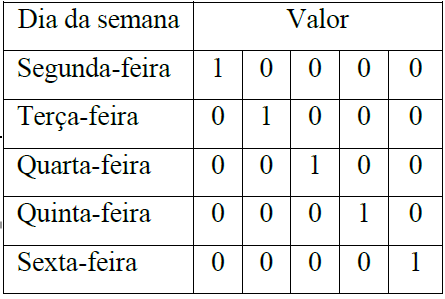
\includegraphics[width=0.40\textwidth]
                		{04-lopes-entradas-dia-semana.png}
                	\caption{Entradas de dia da semana em cofatores.} \subcaption*{ Retirado de \cite{Lopes2008}.}\label{fig:entradasSemanais}}
                \end{figure}
                
	\subsection{Formato final do conjunto de dados}
       \begin{table}[!ht]
            \centering
            \rowcolors{2}{gray!25}{white}
            \begin{tabular}{|c|c|c|} \hline
                \multicolumn{3}{c}{ Estrutura final do conjunto de dados indexados por data: } \\
                \hline
                identificador &	nome da variável					&tipo de variável\\ 
                \hline
                0&	SEMESTRE\_1					&int64 \\
                1&	SEMESTRE\_2					&int64\\
                2&	SEGUNDA						&int64 \\
                3&	TERCA						&int64 \\
                4&	QUARTA						&int64 \\ 
                5&	QUINTA						&int64 \\ 
                6&	SEXTA						&int64 \\ 
                7&	DISTANCIA\_DIA\_ANTERIOR	&	int64 \\ 
                8&	DISTANCIA\_DIA\_POSTERIOR	&	int64 \\
                9&	PERC\_CONCLUSAO\_SEM		&	float64 \\
                10&	PERC\_CONCLUSAO\_MES		&	float64 \\
                11&	PRESSAO\_ATMOSFERICA		&	float64 \\
                12&	TEMPERATURA					&float64 \\ 
                13&	UMIDADE						&int64 \\
                14&	VENTO						&float64\\ 
                15&	VENDAS\_ALMOCO				&int64 \\
                16&	VENDAS\_ALMOCO\_1			&	int64 \\ 
                17&	VENDAS\_ALMOCO\_2			&	int64 \\
                18&	VENDAS\_ALMOCO\_3			&	int64\\ 
                19&	VENDAS\_ALMOCO\_4			&	int64 \\
                20&	VENDAS\_ALMOCO\_5			&	int64 \\ 
                21&	ENTR\_ALMOCO				&	int64\\
                22&	ENTR\_ALMOCO\_1				&int64 \\
                23&	ENTR\_ALMOCO\_2				&int64 \\
                24&	ENTR\_ALMOCO\_3				&int64 \\ 
                25&	ENTR\_ALMOCO\_4				&int64 \\
                26&	ENTR\_ALMOCO\_5				&int64 \\
                27&	ENTR\_JANTAR				&	int64 \\ 
                28&	ENTR\_JANTAR\_1				&int64\\
                29&	ENTR\_JANTAR\_2				&int64 \\ 
                30&	ENTR\_JANTAR\_3				&int64 \\ 
                31&	ENTR\_JANTAR\_4				&int64 \\
                32&	ENTR\_JANTAR\_5				&int64\\
              \hline
            \end{tabular}
            \caption{Estrutura final do conjunto de dados indexados por data}
            \label{table:dataset_final}
        \end{table}
        Por fim, a tabela \ref{table:dataset_final} representa o conjunto de dados estruturados e preparados para o processo de divisão em domínios de treino, validação e teste para o treino dos modelos.
        
        \subsection{Tratamento dos dados para entrada nos modelos}
         	Os dados endógenos, após estruturados na tabela final do conjuntos de dados, ainda passam pelas seguintes transformações:
         	\begin{itemize}
                \item	Calculo do desvio padrão de cada vetor de atributos, e normalização dos valores máximos para o teto de 3x o desvio padrão, e mínimo de 0. 
                \item	Transformação dos dados em escala de 0 e 1
            \end{itemize}
            Os dados exógenos não passam pela transformação em série temporal, portanto os mesmos são tratados de acordo com os passos:
            \begin{itemize}
                \item	Transformação dos dados em escala de 0 e 1.
                \item	Os parâmetros categóricos binários (dias da semana e semestre) já estão escalados por serem categorias binárias.
            \end{itemize}
    	\subsection{Fases Experimentais}
            O processo experimental é realizado em 2 roteiros distintos de divisão do domínio temporal do conjunto de dados, e os resultados obtidos entre as duas fases serão comparados.
            
            O conjunto de dados contemplando o período de 2017 a 2019, é dividido em conjunto de treino, validação e teste da seguinte maneira: 
            
            \paragraph{1º Fase com validação no 1º semestre de 2018 e teste no 1º semestre de 2019}
                Neste roteiro o semestre de validação que compõe o conjunto de dados para o treino backpropagation das redes neurais, contempla o primeiro semestre de 2018 e o conjunto de teste contempla o primeiro semestre de 2019.
                Os dados de 2017 contemplando o 1º e 2º semestre, e 2018 contemplando o 2º semestre, são usados para treino. Os resultados obtidos nesta divisão são usados para validar a hipótese de que os modelos aprendem especificamente a sazonalidade de consumo no primeiro semestre, se saindo melhor nos testes realizados no primeiro semestre de 2019, em comparação aos outros modelos treinados com validação no ano todo de 2018.
                Portanto o conjunto de dados da primeira fase contempla o seguinte domínio:
            \begin{itemize}
                    \item Conjunto de treino dos modelos, contemplando o primeiro e segundo semestre de 2017, e segundo semestre de 2018.
                    \item Conjunto de validação dos modelos, contemplando o primeiro semestre de 2018.
                    \item Conjunto de teste dos modelos, contemplando o primeiro semestre de 2019             
            \end{itemize}
            
            \paragraph{2º Fase com treino em 2017, validação em 2018 e teste em 2019}
                Nesta fase, os conjuntos são divididos conforme sua descrição, e o melhor modelo encontrado passa por uma última etapa de teste no domínio da primeira fase (teste somente no primeiro semestre de 2019).
                As métricas obtidas neste teste são comparadas com o melhor modelo da primeira fase.
    
    \section{Definição e treino dos modelos}
        \subsection{Topologia}
            \paragraph*{Sobre a necessidade de se implementar modelos mistos}
                No conjunto de dados deste trabalho, os dados obtidos se dividem em dados temporais (onde cada registro de consumo e venda trás a informação de seu domínio em um intervalo de 5 dias anteriores) e dados discretos onde temos variáveis categóricas de data para cada registro, e variáveis climáticas, porém sem a aplicação de um intervalo temporal, ou seja, os dados exógenos são discretos, e os endógenos são temporais.
                Portanto é necessária a implementação de modelos específicos para entradas temporais e modelos específicos para as entradas discretas.
                Para a saída final foi implementado um comitê de redes neurais endógenas e exógenas, com um perceptron na saída, recebendo os 2 valores dos modelos endógenos e exógenos para a regressão das saídas das 2 redes ao valor que será a predição do consumo.
         	\subsubsection{Modelos endógenos}
         	\begin{itemize}
                \item	Desenvolvimento das redes perceptron de baixa profundidade para avaliar o aprendizado da rede
                \item	Aumento da profundidade da rede e avaliar as mudanças da função de perda RMSE. 
                \item	Implementação e avaliação dos modelos com redes recorrentes GRU, conforme a figura \ref{fig:gru-arch} que são especialmente desenvolvidos para o aprendizado com memorização de dados, e no caso deste trabalho, podem memorizar as sazonalidades semanais de consumo (em um intervalo de 5 dias).
            \end{itemize}
            \subsubsection{Modelos Mistos : Endógenos e Exógenos}
                \begin{itemize}
                    \item Para os dados temporais (consumo e venda) utilizou-se os melhores modelos endógenos dos experimentos anteriores para as entradas endógenas. 
                    \item Para os dados discretos e categóricos adaptou-se a entrada destes dados para rede perceptron
                    \item  Concatenou-se a saída das 2 redes neurais em um percetron criando um comitê de redes neurais para obter a saída final prevista.
                \end{itemize}
                %TODO-T: FIGURA 24 ESTORANDO MARGEM DO TITULO
	\subsection{Hiperparâmetros : Função de ativação e otimizador}
        Conforme fundamentado no capítulo \label{cap:teoria} na seção "Perceptron", a função de ativação dá a capacidade do perceptron, quando conectado em rede, de resolver problemas lineares e não lineares, agregando adaptação e improviso ao resolver programas que não estão contidos em seus dados de alimentação.
        Portanto para as camadas ocultados das redes neurais MLP desenvolvidas será aplicada a função ReLu e para o neurônio de saída será aplicada a função linear, e o otimizador de treino realiza a função de otimizar o tempo de convergência do reajuste dos pesos à valores ideais, sendo escolhido o otimizador ADAM com taxa de aprendizado defino em 0.001.

    \section{Teste e Métricas}
       A principal métrica de avaliação dos modelos, é a Raiz do Erro Quadrático Médio, obtido pela chamada de função "mean\_squared\_error"\ do framework Tensorflow.Keras utilizado para a modelagem,treino e predição dos modelos de redes neurais.
       
        O coeficiente de correlação de Pearson, obtido pela biblioteca scipy na chamada de função \"scipy.stats.pearsonr(true,pred)"\ e o coeficiente "chi-quadrado" definido como $R^2$ obtido na chamada de função \"scipy.stats.linregress"\ foi utilizado nas etapas de teste para avaliar a proximidade das predições do modelo com o comportamento real de consumo (Se acompanha as quedas e subidas de consumo ao longo do tempo).\newline
       
        Documentou-se, para trabalhos futuros, outras métricas estatísticas obtidas por esta chamada de função como os valores de slope, intercept, p\_value e std\_err.\newline
       
        A chamada de função sns.regplot(x=arr\_true,y=arr\_pred,data=df) da biblioteca seaborn  retorna um gráfico scatter dos valores preditos e reais para a avaliação dos erros, médias e tendencia de previsão.\newline 
       
       Avaliou-se também os erros positivos e negativos entre os valores previstos e reais, para representar quantas refeições seriam descartadas e quantas estariam em falta se a produção de refeições fosse de acordo com as predições do modelo.
       
  % ----------------------------------------------------------
  % \chapter{METODOLOGIA}
  % ----------------------------------------------------------
\chapter{Resultados} \label{cap:resultados}

\TEXTO{Este capítulo descreve os principais resultados experimentais obtidos durante esta pesquisa. Como descrito no capítulo anterior, os experimentos foram conduzidos em duas fases. Contudo, optou-se por apresentar, neste capítulo, apenas os principais resultados obtidos. Um sumário dos demais resultados estão disponíveis no Anexo XX deste documento.}

\TEXTO{Antes de apresentar os resultados, as primeiras seções introduzem a organização dos dados, um breve análise das variáveis e o protocolo experimental, respectivamente.}

\section{Organização do conjunto de dados}
\TODO{descrever, nessa seção, como os dados foram organizados em treino, validação e teste}

    O procedimento de coleta de dados foi realizado de acordo com a metodologia da subseção \ref{subsec:coleta_endogenos} para os dados endógenos, e de acordo com os passos da subseção \ref{subsec:coleta_exógenos} foram obtidos os dados exógenos. 
    Ambos os conjuntos de dados coletados foram estruturados conforme a tabela \ref{table:dataset_final}, contendo um intervalo temporal de registros, desde a data 2017-04-12 (12 de abril de 2017) para o primeiro registro até a data 2019-12-16 (16 de dezembro de 2019) para o último registros, totalizando 514 registros de consumo de refeições em dias letivos.
    
    Conforme a metodologia definida na subseção \ref{subsec:fases_experimentais} este conjunto de dados com o total de 514 registros, foi duplicado para 2 fases experimentais distintas, cada uma com sua organização específica do conjunto de dados.
    
    O conjunto de dados da primeira fase experimental foi organizado de acordo com a figura \ref{fig:case1_timeline}, esta fase tem o conjunto de validação contemplando exclusivamente o primeiro semestre de 2018, indicando uma hipótese de que o primeiro semestre de 2018 tivesse um movimento de consumo e vendas semelhantes ao primeiro semestre de 2019, tal que esta fase seria a ideal para testes envolvendo só o primeiro semestre do conjunto de testes.

    \begin{figure}[htb]
        	\center{
        		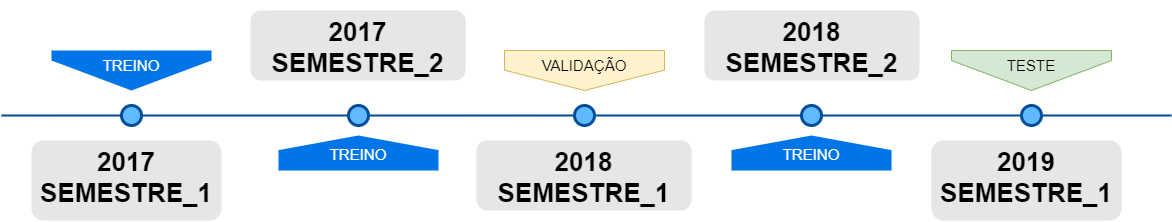
\includegraphics[width=1.0\textwidth]{./Figuras/resultados/case1_timeline.png}
        	
        	\caption{Domínio temporal da 1a fase} \label{fig:case1_timeline} }
        \end{figure}
    E na segunda fase o conjunto de dados foi organizado de acordo com a figura \ref{fig:case2_timeline}, e como esta fase teve um conjunto de validação contemplando 1 ano letivo inteiro, o de 2018, os experimentos de testes dos modelos nesta fase contemplaram o ano todo de 2019.
    
    \begin{figure}[H]
        	\center{
        		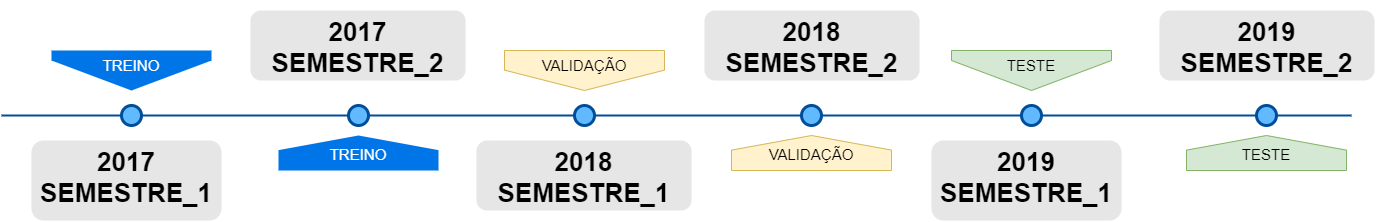
\includegraphics[width=1.0\textwidth]{./Figuras/resultados/case2/case2_dominio.png}
        	
        	\caption{Domínio temporal da 2a fase} \label{fig:case2_timeline} }
        \end{figure}
   
    \paragraph{Dificuldades encontradas e resolvidas}
    A primeira dificuldade encontrada nos experimentos foi um comportamento anômalo do gráfico de previsão, a linha azul na figura \ref{fig:pandas_wrong_indexing} representa uma previsão do modelo que obteve os melhores resultados na primeira fase, e a linha vermelha neste mesmo gráfico representando os valores reais de consumo do primeiro semestre de 2019 também foi anômala. E após uma análise foi descoberto que os registros continham um erro na indexação por data, trocando datas (dia por mês e mês por dia), após a correção da indexação os gráficos de consumo real e previsão produziram resultados melhores e dentro do formato esperado, conforme a figura \ref{fig:pandas_correct_indexing}.
    
    \begin{figure}[htb]
    	\center{
    		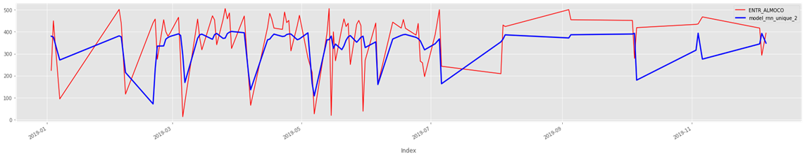
\includegraphics[width=1.0\textwidth]{./Figuras/resultados/pandas_wrong_indexing.png}
    	
    	\caption{Resultado do modelo RNN\_ENDO\_2 obtido sobre o conjunto de dados aleatoriamente ordenado sobre o tempo} \label{fig:pandas_wrong_indexing} }
    \end{figure}
    
    \begin{figure}[htb]
    	\center{
    		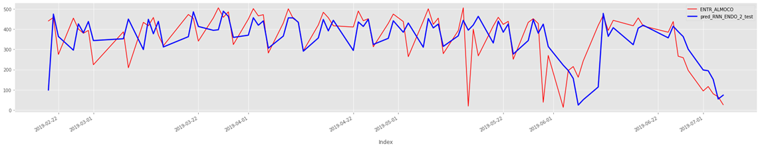
\includegraphics[width=1.0\textwidth]{./Figuras/resultados/pandas_correct_indexing.png}
    	
    	\caption{Resultado do modelo RNN\_ENDO\_2 obtido sobre o conjunto de dados com ordenação corrigida \label{fig:pandas_correct_indexing} }}
    \end{figure}
              
\section{Avaliação das Variáveis}
\TODO{use essa seção se quiser detalhar algo sobre as principais variáveis consideradas, caso contrário, pode excluí-la. Ajuste o texto inicial do capítulo se resolver remover essa seção}

    \paragraph{Estimativas de consumo do restaurante}
        A análise da técnica de estimação de consumo, realizada pela análise subjetiva do consumo da semana anterior, foi feita com o cálculo de 30\% de produção acima do consumo do 5o dia anterior. É possível notar que este método de estimativa é feito para tolerar descartes devido à multa contratual para falta de refeições e que a produção de 30\% de refeições acima do consumo da semana anterior, na figura  \ref{fig:ru_pred} produz um comportamento linear, na linha azul, distante do comportamento real de consumo na linha vermelha. Apesar da estimativa seguir as tendências de quedas e aumento de consumo, a figura \ref{fig:ru_pred_scatter} do gráfico scatter gerado entre a estimava do R.U e o consumo real no ano de 2019, demonstra que a regressão linear (representada pela linha vermelha no gráfico scatter) tem o eixo totalmente descentralizado com a função identidade da estimativa ideal (representada pela diagonal imaginária formada entre a origem do gráfico e o vértice superior direito), gerando também um erro maior do que 30\% no somatório total de refeições descartadas no semestre, ocasionado pelo comportamento oscilatório do consumo, conforme a tabela \ref{table:case2_rupred}.
        {
            \begin{center}
            \begin{minipage}[c]{1.0\textwidth}
                \begin{figure}[H]
                    \center{                    
                        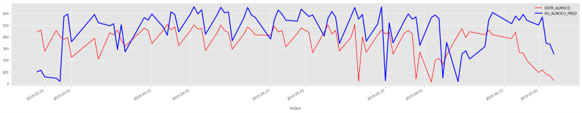
\includegraphics[width=\textwidth]{./Figuras/resultados/case1_ru_pred.png}
                        \caption{Estimativa do restaurante para o ano de 2019} \label{fig:ru_pred} 
                    }
                \end{figure}
            \end{minipage} \hfill %
            
            \begin{minipage}[c]{0.8\textwidth}
                \begin{figure}[H]
                    \center{                    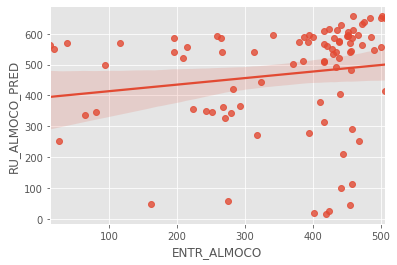
\includegraphics[width=\textwidth]{./Figuras/resultados/case1_ru_pred_scatter.png}
                    \caption{Gráfico scatter da estimativa de consumo do restaurante para o ano de 2019} \label{fig:ru_pred_scatter} }
                \end{figure} 
            \end{minipage} 
            \end{center}
            
            \begin{table}[!ht]
            \centering
            \caption{Métricas da estima de consumo do restaurante para o ano de 2019}
            \label{table:case2_rupred}
            \rowcolors{2}{gray!25}{white}
                \begin{tabular}{|c|c|}
                \rowcolor{gray!50}
                \hline
                \multicolumn{2}{c}{Consumo com margem 30\% acima do 5o dia anterior}\\ \hline     
                TOTAL DE REFEIÇÕES CONSUMIDAS & 58653  \\
                TOTAL DE REFEIÇÕES ESTIMADAS & 76262 \\ 
                CORRELAÇÃO (r)&  0.40067947341844423 \\
                P-value & 2.0845891721642294e-08\\
                RMSE & 191.7620291511743 \\
                SOMA DOS ERROS POSITIVOS & 23412 \\
                SOMA DOS ERROS NEGATIVOS & -5803 \\
                ERRO ABSOLUTO MEDIANO & 133.0 \\
                ERRO ABSOLUTO PERCENTUAL MEDIO & 205.61135949728225\% \\  \hline 
                \end{tabular}
            \end{table}
        }
    \subsection{Análise das variáveis endógenas}
        As variáveis endógenas são os parâmetros temporais de entrada nos modelos MLP e GRU, correspondentes ao domínio de consumo no restaurante.
         % \newpage
        \paragraph*{Consumo do dia vigente em relação às vendas de tickets do dia anterior}
        É possível notar na figura \ref{fig:case1_consumo_vendas_almoco} que as vendas de ticket no período de almoço apresentaram comportamento diferente no ano de 2017 em comparação aos anos seguintes devido à uma limitação imposta pelo restaurante, a partir de 2018, que os alunos comprassem apenas 2 tickets por dia. Possivelmente esta limitação foi dada para aproximar o comportamento de consumo de 1 até 2 dias seguintes à vendas de tickets no dia vigente, esta limitação pode ser interpretada como método de auxílio à gestão para a produção de refeições e para o tratamento de desperdício.
	        
        Mesmo com o valor outlier de 2000 vendas em um único dia, e com a nova limitação de compras de tickets a partir de 2018, o consumo no horário de almoço está fortemente relacionado com as vendas de tickets no período do almoço de 1 dia anterior e nota-se que os alunos se adaptaram à limitação imposta para utilização dos tickets com prazo de validade de 2 dias, conforme o valor de correlação aproximado em 72\% que pode ser conferido na tabela \ref{table:case1_vendas1}.
        
        Há outros fatores não previstos envolvidos, como possíveis falha de registros de vendas no sistema, bem como o outlier de 2000 vendas pode ser interpretado com a migração de sistema e banco de dados de refeições que ocorreu em 2017 da unidade talim do ICT Unifesp para o banco de dados do Hospital São Paulo, possivelmente também foram importadas vendas do sistema antigo sem a diferenciação de datas. A soma de vendas de tickets no horário do almoço, totalizou 242282 tickets vendidos no período do almoço, em todo o conjunto de dados de 514 registros, e a soma de passagens de alunos pela catraca do restaurante também no período do almoço, sendo o valor real de consumo, totalizou 163752 refeições. Apesar de notória a diferença de 78.530 tickets vendidos acima do consumo real não foi possível investigar neste trabalho as causas desta diferença, ressaltando que estes valores foram obtidos no conjunto original de dados fornecidos pelo fiscal de contrato do R.U do ICT Unifesp através de consulta solicitada via e-mail para este fiscal.

	       {
	       \begin{center} 
    	        \begin{minipage}[c]{1.0\textwidth}
    	            \begin{figure}[H]
                    	\center{                    		        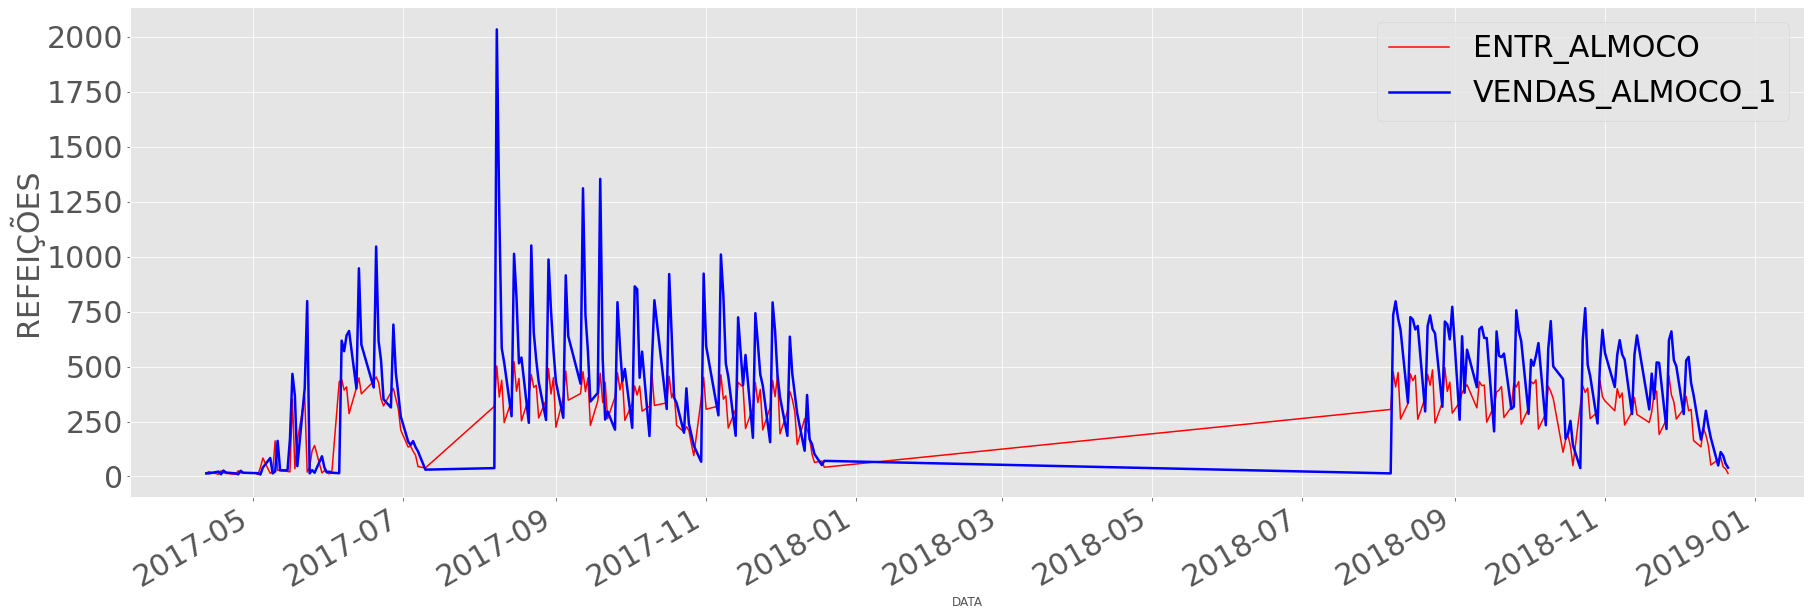
\includegraphics[width=1.0\textwidth]{./Figuras/resultados/case1_consumo_vendas_almoco.png}
                    	\caption{Correlação entre consumo e vendas de almoço.} \label{fig:case1_consumo_vendas_almoco} 
                    	}
                    \end{figure}
                \end{minipage} \hfill %
                \begin{minipage}[c]{0.3\textwidth}
                    \begin{figure}[H]
                    	\center{                    		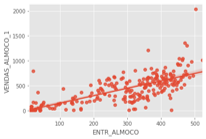
\includegraphics[width=1.0\textwidth]{./Figuras/resultados/case1_scatter_consumo_vendas_almoco.png}
                    	\caption{Gráfico Scatter entre consumo e vendas de almoço.} \label{fig:case1_scatter_consumo_vendas_almoco} }
                    \end{figure}
                \end{minipage} 
            \end{center}
            }
                
           \begin{table}[!ht]
           \centering
           \caption{Comparação de consumo com um dia anterior}
             \rowcolors{2}{gray!25}{white}
             \begin{tabular}{|c|c|}\hline
                \multicolumn{2}{c}{CONSUMO EM RELAÇÃO ÀS VENDAS DE 1 DIA ANTERIOR}\\ \hline
                CORRELAÇÃO (r) &  0.7255528038157009\\
                P-value &5.399561176138223e-41\\
                RMSE & 260.5399426736619\\
                TOTAL DE REFEIÇÕES PROJETADAS & 104694\\ 
                TOTAL DE REFEIÇÕES CONSUMIDAS & 69544\\
                TOTAL DE REFEIÇÕES SUB PROJETADAS & -4703\\
                TOTAL DE REFEIÇÕES SUPER PROJETADAS & 39853\\
                ERRO ABSOLUTO MEDIANO & 139.0\\
                ERRO ABSOLUTO PERCENTUAL MEDIO & 90.18\\\hline
            \end{tabular} \label{table:case1_vendas1} \end{table}

            \paragraph*{Normalização e escala de features}
                O processo de normalização e escala é demonstrado nesta seção com a feature de vendas de tickets de 1 dia anterior, pois entre todas as features esta é a que produziu outliers com maior destaque.
                A normalização dos dados é feita com o teto de 3x o desvio padrão médio, logo o pico de 2000 vendas foi normalizado para o valor arredondado de 1356 refeições e mesmo com a normalização, o comportamento linear desta feature, conforme figura \ref{fig:feature_sem_outliers}, se manteve.   
                E após a normalização foi realizada a aplicação da escala de 0 a 1 na feature e conforme é observado na figura  \ref{fig:feature_sem_outliers_escalada}, o comportamento linear da feature também se manteve.

                {
                    \begin{center}
                        \begin{minipage}[b]{1.0\textwidth}
                        \begin{figure}[H]
                        	\center{
                            	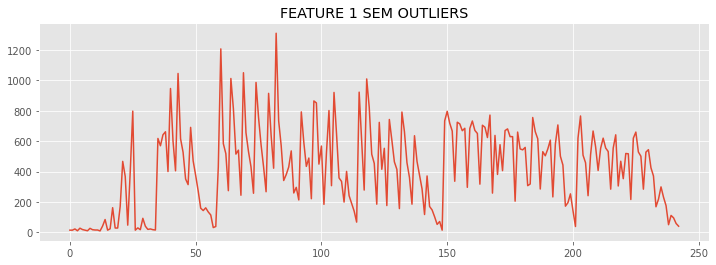
\includegraphics[width=1.0\textwidth]{./Figuras/resultados/feature_sem_outliers.png}
                            	\caption{Vendas de tickets normalizados com teto de 3x o desvio padrão.}
                            	\label{fig:feature_sem_outliers}
                        	}
                        \end{figure}
                        \end{minipage} \hfill %
                        
                        \begin{minipage}[b]{1.0\textwidth}
                        \begin{figure}[H]
                        	\center
                        	{                    		
                            	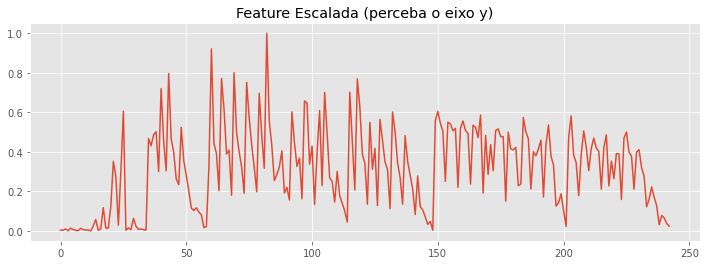
\includegraphics[width=1.0\textwidth]{./Figuras/resultados/feature_sem_outliers_escalada.png}
                            	\caption{Vendas de tickets escalada entre 0 a 1.} \label{fig:feature_sem_outliers_escalada} 
                        	}
                        \end{figure}
                        \end{minipage}
                    \end{center}
                }
                Este processo de normalização e escala foi realizado para todas as features endógenas e para as features climáticas.
        	   % \newpage
        	   
                \paragraph{Consumo atual em relação ao consumo do jantar de 1 dia anterior.}
                
                    Apesar de que os alunos que consomem refeições no almoço geralmente são de período e de grade horária diferente dos alunos que consomem o jantar no período da noite, nota-se uma relação evidente entre os 2 consumos, evidenciada pelo comportamento linear na figura \ref{fig:case1_consumo_jantar} com correlação (r) = 0.7655, e pela regressão linear entre esses 2 consumos na figura  \ref{fig:case1_consumo_jantar_scatter}, não foi possível encontrar uma causa evidente para este efeito anômalo.
                    
                    {\begin{center} 
                    \begin{minipage}[c]{1.0\textwidth}
                    \begin{figure}[H]
                    	\center{
                    	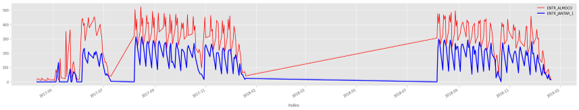
\includegraphics[width=1.0\textwidth]{./Figuras/resultados/case1_consumo_jantar.png}
                    	\caption{Correlação de consumo de almoço e jantar de 1 dia anterior.} 
                    	\label{fig:case1_consumo_jantar} }
                    \end{figure} 
                    \end{minipage}\hfill %
                    
                    \begin{minipage}[c]{0.3\textwidth}
                    \begin{figure}[H]
                    	\center{                    		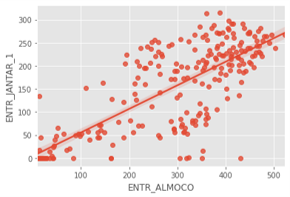
\includegraphics[width=1.0\textwidth]{./Figuras/resultados/case1_consumo_jantar_scatter.png}
                    	\caption{Gráfico Scatter entre consumo e jantar de 1 dia anterior.} 
                    	\label{fig:case1_consumo_jantar_scatter} }
                    \end{figure}
                    \end{minipage} \end{center} }
            
    	    \paragraph{Análise da sazonalidade semanal}
    	        Os gráficos de consumo a seguir da figura  \ref{fig:case1_violinplot_segunda}, representando a segunda-feira,  até a figura \ref{fig:case1_violinplot_sexta} , representando a sexta-feira,  são gerados para as features categóricas binárias, com a funcionalidade violin-plot da biblioteca seaborn, própria para distribuição de variáveis categóricas-binárias em um dataset.
    	        O violino azul com o valor 1 representa a distribuição do consumo ao longo do conjunto total de dados.
    	        O violino com valor zero pode ser ignorado e é um retorno padrão no gráfico da ferramenta, representando o complemento do consumo para o dia da semana considerado.
    	        Nas sextas feiras, o consumo teve escala de distribuição menor para todo o conjunto 2019. Foi notório que apesar da alternância de grades horárias durante a troca de semestres no ano de 2019, os dias de terça e quinta feira concentraram o maior movimento de consumo.
    	       %\newpage
    	       \begin{center}    
    	        \begin{minipage}[c]{0.45\textwidth}
    	         \begin{figure}[H]
                	\center{                		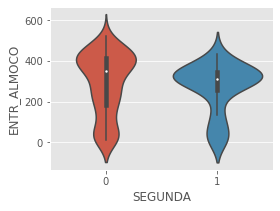
\includegraphics[width=\textwidth]{./Figuras/resultados/case1_segunda.png}
                	\caption{Gráfico violino da distribuição do consumo na segunda feira.} \label{fig:case1_violinplot_segunda} }
                \end{figure}\end{minipage} \hfill %
                      \begin{minipage}[c]{0.45\textwidth}
                \begin{figure}[H]
                	\center{                		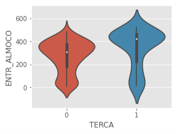
\includegraphics[width=\textwidth]{./Figuras/resultados/case1_terca.png}
                	\caption{Gráfico violino da distribuição do consumo na terça feira.} \label{fig:case1_violinplot_terca} }
                \end{figure} \end{minipage}
                 \begin{minipage}[c]{0.45\textwidth} 
                \begin{figure}[H]
                	\center{                		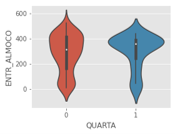
\includegraphics[width=\textwidth]{./Figuras/resultados/case1_quarta.png}
                	\caption{Gráfico violino da distribuição do consumo na quarta feira.	} \label{fig:case1_violinplot_quarta} }
                \end{figure}\end{minipage} \hfill %
                      \begin{minipage}[c]{0.45\textwidth}
                \begin{figure}[H]
                	\center{                		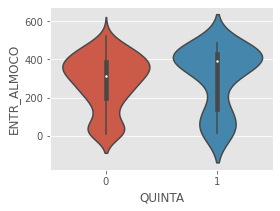
\includegraphics[width=\textwidth]{./Figuras/resultados/case1_quinta.png}
                	\caption{Gráfico violino da distribuição do consumo na quinta feira.} \label{fig:case1_violinplot_quinta} }
                \end{figure}\end{minipage} %
                        \begin{minipage}[c]{0.45\textwidth}
                \begin{figure}[H]
                	\center{                		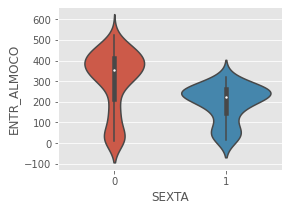
\includegraphics[width=\textwidth]{./Figuras/resultados/case1_sexta.png}
                	\caption{Gráfico violino da distribuição do consumo na sexta feira.} \label{fig:case1_violinplot_sexta} }
                \end{figure}
                \end{minipage} \end{center}
    \subsection{Análise das variáveis exógenas}
        As variáveis exógenas correspondem aos parâmetros, de domínio discreto, que são utilizados exclusivamente nos modelos de redes neurais mistos, e são lidos pelas camadas MLP destes modelos.
        \paragraph{Consumo atual em relação ao avanço do semestre}
        Para esta análise foi necessário restringir o domínio de análise para 1 semestre, o consumo em relação ao avanço do semestre teve queda abrupta nos ultimos dias do semestre, portanto a correlação dos conjuntos de dados das figuras \ref{fig:case1_perc_sem} e \ref{fig:case1_perc_sem_scatter} obteve valor negativo.
        {
        \begin{center} 
        
            \begin{minipage}[c]{1.0\textwidth}
                \begin{figure}[H]
                	\center{                    		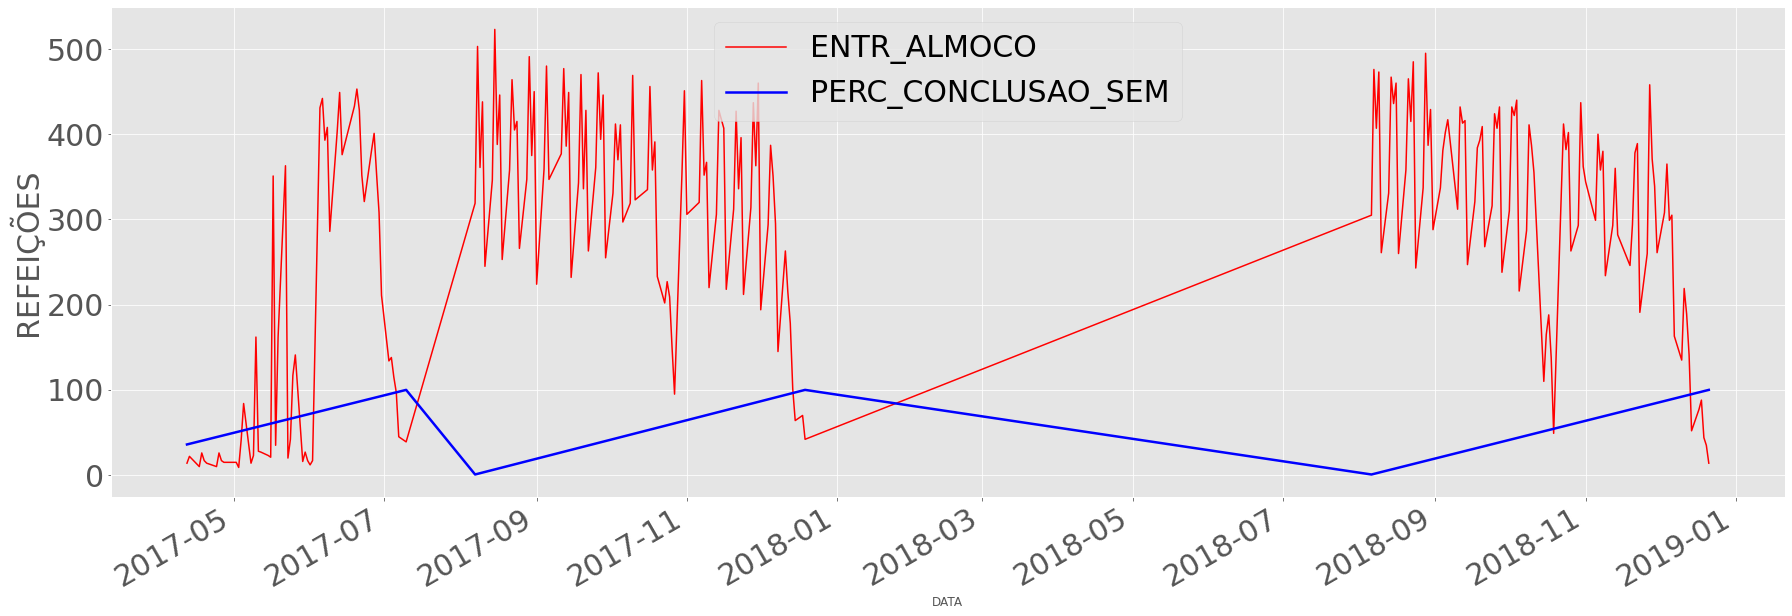
\includegraphics[width=\textwidth]{./Figuras/resultados/case1_perc_sem.png}
                	\caption{1a Fase : Relação da distribuição do consumo com o avanço do semestre, Correlação (r) = -0.35}
                	\label{fig:case1_perc_sem}
                	}
                \end{figure}  
            \end{minipage} \hfill %
        
            \begin{minipage}[c]{0.5\textwidth}
                \begin{figure}[H]
                	\center{                		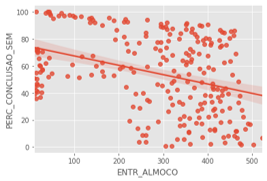
\includegraphics[width=\textwidth]{./Figuras/resultados/case1_perc_sem_scatter.png}
                	\caption{Gráfico scatter da distribuição do consumo com o avanço do semestre.} \label{fig:case1_perc_sem_scatter}
                	}
                \end{figure}
            \end{minipage} 
        \end{center} 
        }

\section{Protocolo Experimental}
\TODO{faça um resumo sobre as duas fases e as principais diferenças entre elas. Na sequência, detalhe os detalhes do principal modelo obtido (o com melhor resultado de predição)}
    
    \subsection{Avaliação do aprendizado do problema da predição de refeições por meio de redes neurais MLP}
        \paragraph{Ajuste empírico de topologia do primeiro modelo perceptron}
        O primeiro experimento com redes neurais realizado na primeira fase experimental, avaliou a capacidade de aprendizado do modelo perceptron sobre a sazonalidade dos dados endógenos, referentes ao domínio de consumo de refeições no R.U, verificando se o comportamento de consumo no restaurante pôde ser aprendido por este tipo de rede neural, portanto foi definida 1 rede neural inicial perceptron com apenas 1 camada oculta contendo 1 neurônio para 15 parâmetros de entrada (mesmo número de parâmetros endógenos) e com 1 neurônio de saída, denominada de MLP1.
        
        Os parâmetros endógenos correspondem à uma série temporal de intervalo de 5 dias anteriores para consumo de refeições no período do almoço, jantar e de vendas de tickets no período do almoço.
        O modelo foi denominado MLP1, sua ilustração pode ser visualizada na figura \ref{fig:case1_mlp1} obtida através da ferramenta NETRON. Cada camada do modelo MLP1 corresponde à um bloco com título \textbf{Dense} nesta figura, a primeira aresta da figura entre o bloco input e InputLayer demonstra as 3 séries temporais dos parâmetros de entrada, com intervalo de 5 dias passados cada. \textbf{ENTR\_ALMOCO, ENTR\_JANTAR e VENDAS\_ALMOCO}. O bloco Flatten converte cada dia de entrada das séries temporais em um parâmetro de entrada da rede neural MLP, conforme modelo conceitual do trabalho de \citeonline{Lopes2008} ilustrado na figura \ref{fig:mlp-lopes} que utiliza apenas 1 parâmetro endógeno com intervalo temporal também de 5 dias. A primeira camada oculta desta rede pode ser visualizada no primeiro bloco dense da figura que demonstra a função de ativação ReLu deste neurônio, e o número de unidades desta camada sendo 1.
        A camada de saída é o último bloco da figura, também com 1 unidade, e como a função de ativação é linear, ela não é exibida na descrição do bloco.
        \begin{figure}[H]
        \center{
        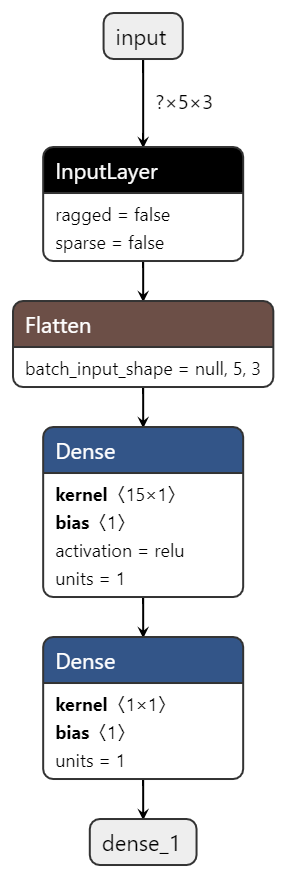
\includegraphics[width=0.3\textwidth]{./Figuras/resultados/case1_MLP1_validated.png}
        	\caption{Topologia do modelo MLP1, Ferramenta NETRON} 
        	\label{fig:case1_mlp1}
        }
        \end{figure}
        O treino deste modelo foi executado, obtendo RMSE com o valor 130,62 sobre o conjunto de validação, neste caso da primeira fase sendo os dados do primeiro semestre de 2018, e é possível notar figura \ref{fig:case1_mlp1_train} que as linhas da função de perda e treino convergiram à um processo de overfitting e não demonstraram aprendizado significante deste modelo sobre o conjunto de validação.
        \begin{figure}[H]
        	\center{
        	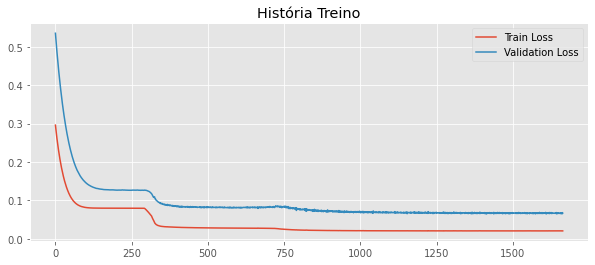
\includegraphics[width=0.8\textwidth]{./Figuras/resultados/case1_mlp1_train.png}
        	\caption{Gráfico de treino do modelo MLP1, RMSE = 130,62}
        	\label{fig:case1_mlp1_train}
        	}
        \end{figure}
        
        Portanto foi aumentada a profundidade do modelo MLP1 obtendo-se o modelo MLP2 com topologia ilustrada na figura  \ref{fig:case1_mlp2}, e após o treino deste modelo foi possível notar a diminuição do RMSE (Raiz do erro quadrático médio) para o valor de 107.97, observado na figura \ref{fig:case1_mlp2_train}. Validando a hipótese de que a predição do consumo no restaurante, pode ser aprendida por modelos simples de redes neurais, e portanto a pesquisa seguiu com a definição de novos modelos demonstrados na próxima subseção.
        \begin{figure}[H]
        	\center{
        		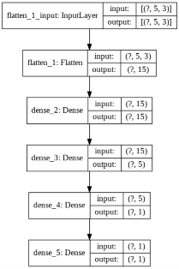
\includegraphics[width=0.3\textwidth]{./Figuras/resultados/case1_mlp2.png}
        	\caption{Topologia do modelo MLP2} \label{fig:case1_mlp2} }
        \end{figure}
        \begin{figure}[H]
        	\center{
        		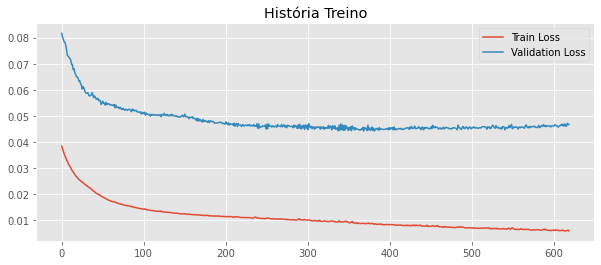
\includegraphics[width=1.0\textwidth]{./Figuras/resultados/case1_mlp2_train.png}
        	\caption{Gráfico de treino do modelo MLP2. RMSE = 107.97}
        	\label{fig:case1_mlp2_train} }
        \end{figure}
    \subsection{Definições das topologias dos modelos}
        \paragraph{Modelo endógeno MLP\_ENDO\_1}
            O primeiro modelo experimental MLP para obtenção das predições tem topologia definida na figura \ref{fig:case1_mlp_endo1}, denominado MLP\_ENDO\_1, este modelo tem 64 neurônios na primeira camada oculta e 32 neurônios na segunda camada oculta, e assim como todos os outros modelos, 1 neurônio na camada de saída. Ressaltando que a metodologia do cap \ref{cap:metodos} define que para os modelos MLP as camadas ocultas utilizam função de ativação ReLu e função de saída Linear.
            \begin{figure}[H]
            	\center{                		
            	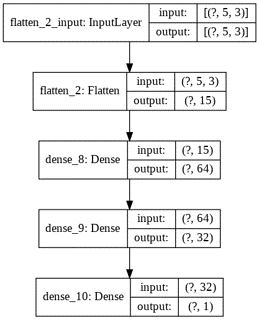
\includegraphics[width=0.25\textwidth]{./Figuras/resultados/case1_mlp_endo1.png}
            	\caption{Topologia do modelo MLP\_ENDO\_1} 
            	\label{fig:case1_mlp_endo1} 
            	}
            \end{figure}
            
         \paragraph{Modelo endógeno GRU RNN\_ENDO\_1}
            Este primeiro modelo experimental GRU foi definido com 16 unidades GRU, com topologia conceitual definida de acordo com a figura \ref{fig:gru-arch} no capítulo de fundamentação teórica \textbf{MLP\_ENDO\_1} e tem um neurônio perpcetron para emissão do sinal de saída, representado pelo bloco\textbf{Dense} na figura \ref{fig:case1_rnn_endo1}
            \begin{figure}[H]
              \center{
                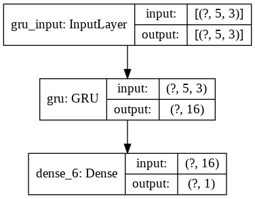
\includegraphics[width=0.25\textwidth]{./Figuras/resultados/case1_rnn_endo1.png}
                \caption{Topologia do modelo RNN\_ENDO\_1} \label{fig:case1_rnn_endo1} }
            \end{figure}
         
         \paragraph{Modelo endógeno GRU RNN\_ENDO\_2}
           Foi definido uma segunda reconfiguração do modelo GRU, RNN\_ENDO\_2, com o aumento da profundidade de unidades do modelo anterior RNN\_ENDO\_1, em formato regressivo de 16 unidades na primeira camada, 8 unidades na segunda e 4 na terceira, e com a inclusão do recurso Dropout entre as unidades para eliminar unidades com pesos negativos no grafo denso da rede, observado na figura \ref{fig:case1_rnn_endo2} realizando a poda de unidades não relevantes durante o treino.
            \begin{figure}[H]
              \center{
                  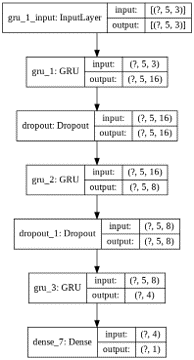
\includegraphics[width=0.20\textwidth]{./Figuras/resultados/case1_rnn_endo2.png}
                  \caption{Topologia do modelo RNN\_ENDO\_2} 
                  \label{fig:case1_rnn_endo2} 
              }
            \end{figure}
        \paragraph{Modelo misto RNN\_EXO\_1}
            Interpretando o digrama do primeiro modelo misto,  \textbf{RNN\_EXO\_1}, na figura \ref{fig:case1_rnn_exo_1}o bloco com título GRU à esquerda na figura de topologia do modelo, trata as entradas endógenas (temporais), assim como exemplificado nos modelos GRU endógenos. O bloco com título \textbf{Dense} é uma rede MLP que recebe um input com 10 parâmetros de 1 dimensão, portanto todos discretos, correspondendo aos 4 parâmetros climáticos (temperatura, umidade, pressão e vento), 1 parâmetro para o dia da semana vigente, 1 para o semestre vigente e 4 parâmetros de controle do calendário (distancia da data anterior, posterior, avanço do semestre, avanço do mês). A saída dos blocos GRU e MLP são concatenadas e tratadas pelo bloco MLP de saída.
            \begin{figure}[H]
              \center{
                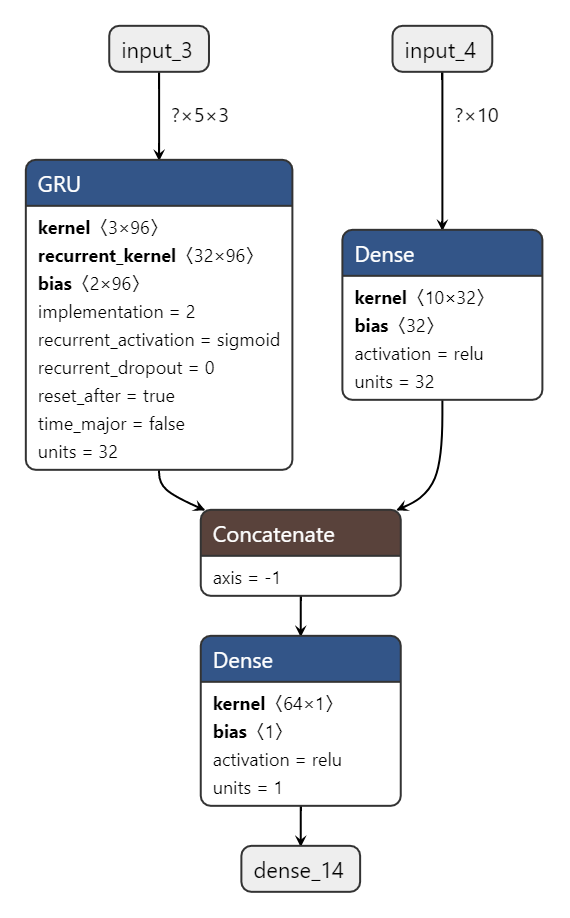
\includegraphics[width=0.7\textwidth]{./Figuras/resultados/case1_rnn_exo_1.png}
                \caption{Topologia do modelo RNN\_EXO\_1} \label{fig:case1_rnn_exo_1} }
            \end{figure}
            
        \paragraph{Modelo misto RNN\_EXO\_2}
         O Segundo modelo misto foi definido com o aumento da profundidade das camadas GRU e MLP do modelo anterior, conforme observado na figura \ref{fig:case1_rnn_exo_2} foram acrescentadas 1 camada GRU e 1 camada MLP (Dense).
            \begin{figure}[H]
              \center{
                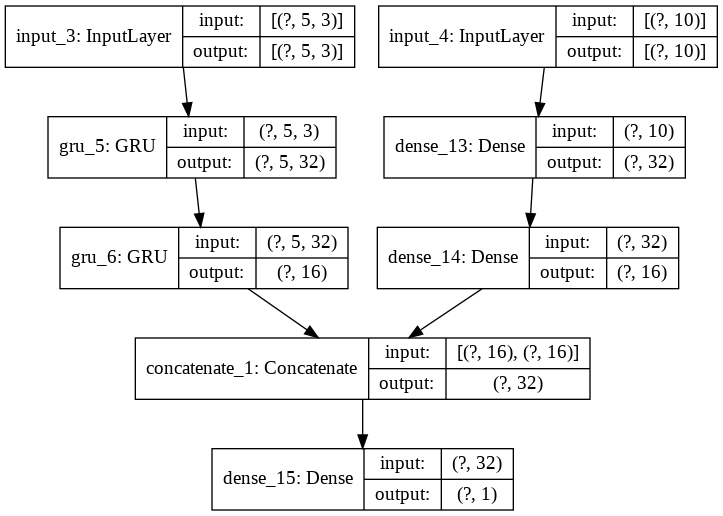
\includegraphics[width=0.6\textwidth]{./Figuras/resultados/case1_rnn_exo_2.png}
              \caption{Topologia do modelo RNN\_EXO\_2}  \label{fig:case1_rnn_exo_2} }
            \end{figure}
        
        \paragraph{Modelo misto RNN\_EXO\_3}
        Para o terceiro e último modelo misto, representado na figura \ref{fig:case1_rnn_exo_3}, foi feita uma reconfiguração do modelo misto anterior com a utilização do recurso dropout nas saídas das camadas GRU, que realiza podas de conexões com pesos negativos.
        \begin{figure}[H]
          \center{
          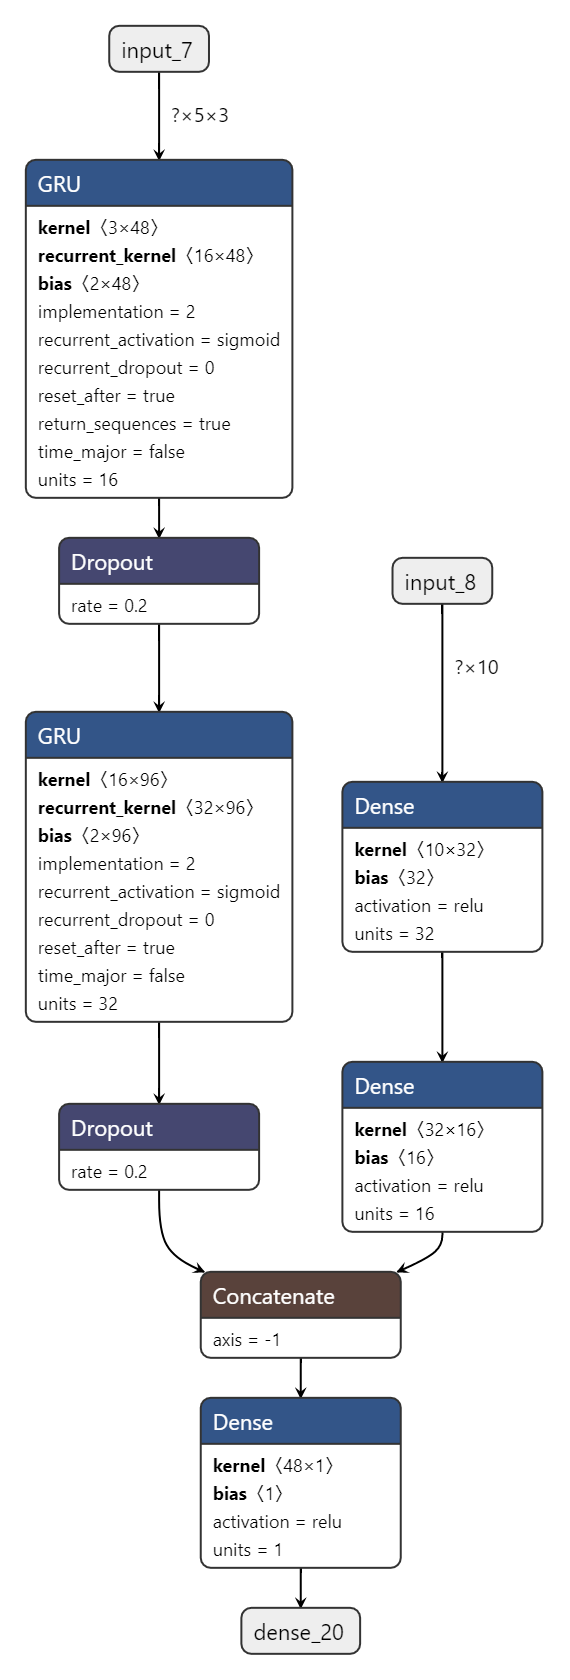
\includegraphics[width=0.5\textwidth]{./Figuras/resultados/case1_rnn_exo_3.png}
          \caption{Topologia do modelo RNN\_EXO\_3} \label{fig:case1_rnn_exo_3} 
          }
        \end{figure}
    \subsection{Diferenças principais dos resultados entre as fases experimentais}
        \paragraph{Diferenças entre os melhores modelos}
        Para os experimentos da 1a fase, o modelo que produziu o menor RMSE no conjunto de testes com vantagem em todas as outras métricas foi o modelo endógeno, RNN\_ENDO\_2, com algumas anomalias de predição observadas na figura \ref{fig:case1_rnn_endo2_test_dates}.
        \begin{figure}[H]
          \center{
            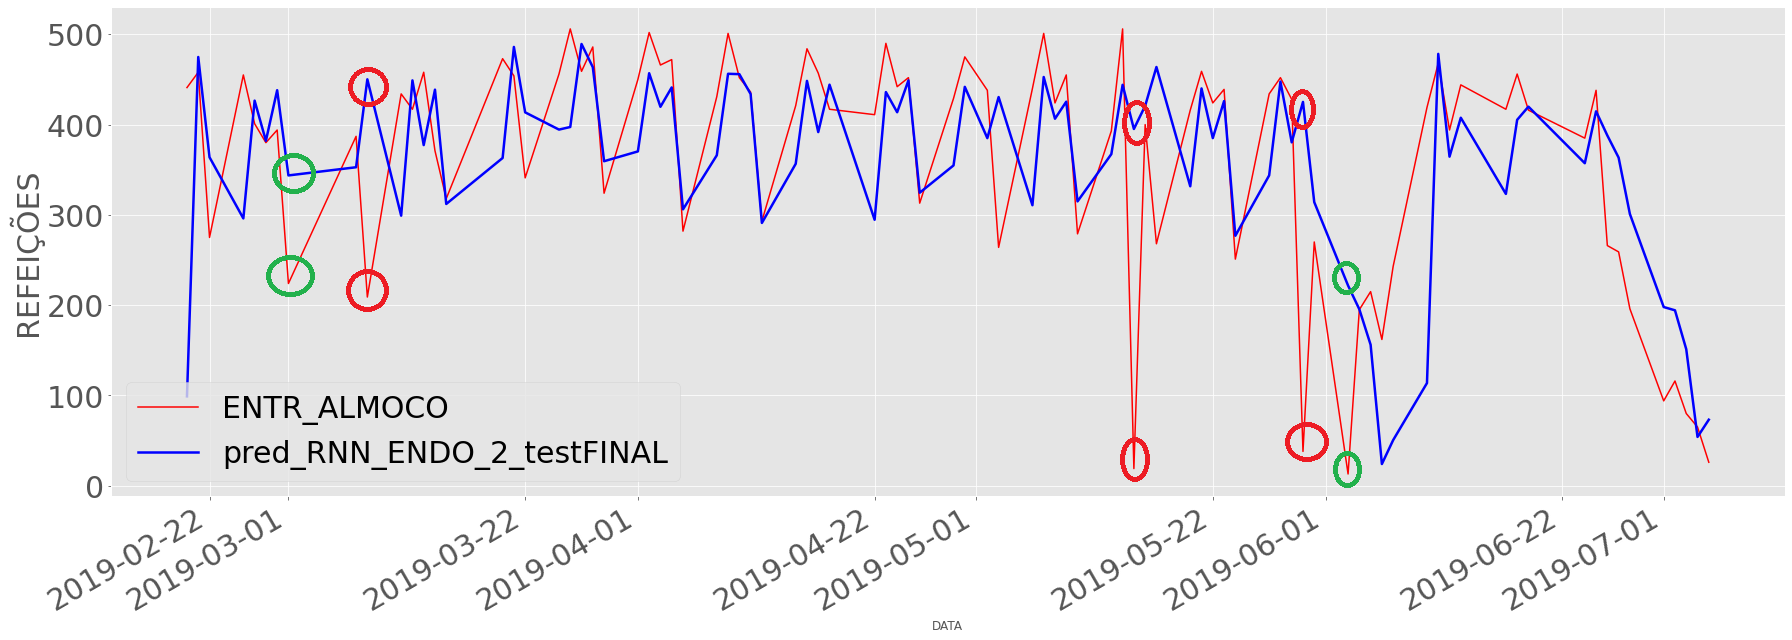
\includegraphics[width=1.0\textwidth]{./Figuras/resultados/case1_rnn_endo2_test_dates.png}
          \caption{Analise de anomalias preditivas do RNN\_ENDO\_2} \label{fig:case1_rnn_endo2_test_dates} }
        \end{figure}
        
        Os pontos verdes outliers representam predições que corresponderam a tendência de alta ou baixa de consumo mas com erros discrepante, e os pontos vermelhos representam predições com tendência inversa ao consumo.
        As justificativas para a predição dentro da tendência, se encontram na tabela \ref{table:rnn_endo_2_green}, denotando datas especiais que não poderiam corresponder ao processo de aprendizado do modelo.
            \begin{table}[!ht]
                \centering
                \caption{Erros de predições do modelo RNN\_ENDO\_2 na 1a fase}
                \label{table:rnn_endo_2_green}
                \rowcolors{2}{gray!25}{white}
                 \begin{tabular}{|c|c|c|}
                 \rowcolor{gray!50}
                 \hline 
                Data & Consumo & Justificativa\\ \hline    
                01/03/2019 (sexta feira)    & 224 & Sexta Feira pré - carnaval\\
                03/06/2019 (segunda feira)  &  13 & Segunda Feira pós paralisação estudantil\\ \hline 
                \end{tabular} 
            \end{table}
            
        As justificativas para previsões onde o modelo seguiu tendência oposta ao consumo também corresponderam à datas especiais, conferidas na tabela \ref{table:rnn_endo_2_red}.
            \begin{table}[!ht]
                \caption{Anomalias de predições do modelo RNN\_ENDO\_2 na 1a fase}
                \label{table:rnn_endo_2_red}
                \rowcolors{2}{gray!25}{white}
                 \begin{tabular}{|c|c|c|}
                 \rowcolor{gray!50}
                 \hline
                Data & Consumo & Justificativa \\
                08/03/2019 (sexta feira)   & 209 &Sexta Feira pós - carnaval\\
                15/05/2019 (quarta feira)   & 19  & Paralisação estudantil na praça Afonso Pena\\
                30/05/2019 (quinta feira)   &  38  & Paralisação estudantil na Praça Afonso pena\\
                \hline 
                \end{tabular} 
            \end{table}
        
        Nas métricas deste modelo, é observado na tabela \ref{table:rnn_endo_2_test} que a soma dos erros positivos, correspondeu à um descarte de aproximadamente 3479 refeiçoes, e o erro quadrático médio de previsão foi de aproximadamente 108 refeições.
            \begin{table}[!ht]
                \centering
                \rowcolors{2}{gray!25}{white}
                \caption{Métricas do melhor modelo:  RNN\_ENDO\_2 }
                \label{table:rnn_endo_2_test}
                \begin{tabular}{|c|c|}
                \rowcolor{gray!50}
                \hline
                Melhor modelo: &   RNN\_ENDO\_2: \\ \hline
                Total\_Consumidas & 31962 \\ 
                Total\_Previstas & 31465,61133 \\
                Erro\_Total\_Previsao & -496,3886719 \\
                Percentual\_Erro\_Total & -1,5530\% \\\
                Correlação & 0,595439895 \\
                P-value & 9,42215E-10    \\
                RMSE &  108,0663015\\
                Soma dos erros Negativos & -2982,567947 \\
                Soma dos erros Positivos & 3478,957266\\
                ERRO\_ABS\_MEDIANO & 46,70721436 \\ 
                ERRO\_ABSOLUTO\_PERCENTUAL\_MEDIO & 74,93539002 \\ 
                \hline
                \end{tabular}
            \end{table}
        
        Já na segunda fase, todos os modelos obtiveram melhoras no erro de treino sobre o conjunto de validação, e foi obtido o modelo com as melhores predições do trabalho, o modelo misto \textbf{RNN\_EXO\_1} detalhado em sua própria seção a seguir.
        É importante notar que as 2 fases produziram melhores modelos de classes distintas, a primeira com um modelo que utiliza apenas dados endógenos, e que contempla um conjunto de validação e teste com amplitude de apenas 1 semestre, e a segunda com um modelo que utiliza dados temporais e discretos, e que utiliza conjunto de validação e teste com amplitude de 1 ano.
        Isso denota que resultados melhores foram conquistados sem nenhuma alteração de parâmetros e hiper-parâmetros nos modelos, alterando-se apenas a organização temporal dos conjuntos de dados.
        
        Durante o teste de todos os modelos, apenas o primeiro semestre contemplou datas especiais onde estes modelos produziram anomalias de previsões, ilustrado como exemplo na figura \ref{fig:case1_rnn_endo2_test_dates}.

\section{Resultados com o Modelo RNN\_EXO\_1}
\TODO{Nessa seção apresente os resultados do melhor modelo. Se quiser, pode dividir em subseções}
    Este modelo, representado na figura \ref{fig:case1_rnn_exo_1} obteve os melhores resultados de todo este trabalho quando foi treinando na segunda fase experimental.
    É notório sua melhoria de resultados com uma única mudança da organização dos conjuntos de dados entre as fases experimentais.
    
    \subsection{Comparativo do treino entre as duas fases}
     Nota-se que este modelo produziu um gráfico função de perda durante o treino, com comportamento oscilatório pior, convergindo mais rapidamente à um overfitting, na primeira fase, ilustrado na figura \ref{fig:case1_rnn_exo_1_train} em comparação ao treino com melhores resultados na segunda fase, ilustrado na figura \ref{fig:case2_rnn_exo1_train}. É notório também a diferença das métricas RMSE entre estes 2 treinos, produzindo um resultado melhor na segunda fase, de RMSE = 109,97 em comparação ao resultado da primeira fase de RMSE = 132,94.
     
     \paragraph{Resultados de treino e validação para a primeira fase}
     {
        \begin{center} \begin{minipage}[c]{1.0\textwidth}
        \begin{figure}[H]
        \center{                    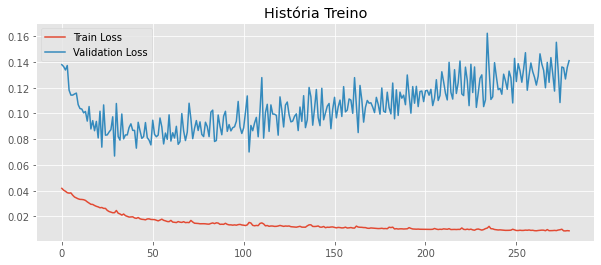
\includegraphics[width=\textwidth]{./Figuras/resultados/case1_rnn_exo_1_train.png}
        \caption{Treino do modelo RNN\_EXO\_1 na 1a fase, RMSE = 132.94} \label{fig:case1_rnn_exo_1_train} }
        \end{figure}
        \end{minipage} \hfill %
        \end{center} 
      }
     
    \paragraph{Resultados de treino e validação para a segunda fase}
    {\begin{center} \begin{minipage}[b]{1.0\textwidth}
        \begin{figure}[H]
          \center{
            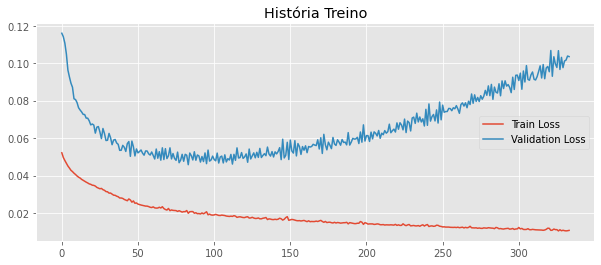
\includegraphics[width=\textwidth]{./Figuras/resultados/case2/case2_rnn_exo1_train.png}
          \caption{Gráfico de treino do modelo RNN\_EXO\_1 na 2a fase, RMSE = 109.97} \label{fig:case2_rnn_exo1_train} }
        \end{figure}\end{minipage} \hfill %
        \end{center} }
    
    \subsection{Comparativo de teste do modelo no primeiro semestre, entre as 2 fases}
        Como este modelo treinado na segunda fase obteve os melhores resultados do trabalho, foram recalculadas as métricas para o teste de modelo dentro do domínio do primeiro semestre de 2019 para realizar uma comparação justa com sua versão treinada e testada também no primeiro semestre de 2019 na primeira fase.
        
        A tabela \ref{table:case1_rnn_exo_1} demonstra que o RMSE de teste do modelo treinado na primeira fase foi notoriamente maior, e portanto pior, do que o RMSE treinado na segunda fase de acordo com a tabela \ref{table:case2_rnn_exo_2_incase1}. O RMSE sendo menor no treino deste modelo na segunda fase já trás uma melhoria em todas as outras métricas em comparação com o seu treino na primeira fase.
        A soma dos erros positivos de predições também foi menor na segunda fase, o que impacta menor em descarte de refeições.
        O RMSE deste modelo testado na primeira fase e alcançando RMSE = 106,2080 também se saiu melhor do que o melhor modelo da primeira fase, o RNN\_ENDO\_2 que alcançou RMSE = 108,06.
        
        O gráfico scatter do modelo treinado na primeira fase, conforme figura \ref{fig:case1_rnn_exo_1_test_scatter} também se saiu pior, mais distante da borda superior direita do gráfico, em relação ao scatter do modelo treinado na segunda fase conforme a figura \ref{fig:case2_rnn_exo2_test_incase1_scatter}.
        
        Por fim na comparativa entre os gráficos de predição, o modelo RNN\_EXO\_1 treinado na primeira fase produziu predições piores, e não aprendeu a sazonalidade semanal do consumo, como pode ser observado na figura \ref{fig:case1_rnn_exo_1_test}, é possível notar também, na tabela  \ref{table:case1_rnn_exo_1}, que a correlação entre os valores previstos e o consumo real, bem como o valor $R^2$ foi inferior em comparação às métricas do modelo treinado na segunda fase, e que este modelo treinado na segunda fase aprendeu melhor a sazonalidade semanal e mensal do consumo como pode ser observado na figura \ref{fig:case2_rnn_exo2_test_incase1}.
        
        \paragraph{Teste para o 1o semestre, treino na 1a fase}
            {
    	    \begin{center} 
    	        \begin{minipage}[c]{1.0\textwidth}
                  \begin{figure}[H]
                      \center{                    \includegraphics[width=\textwidth]{./Figuras/resultados/case1_rnn_exo_1_test.png}
                      \caption{Teste do modelo RNN\_EXO\_1, 1a fase} 
                      \label{fig:case1_rnn_exo_1_test} }
                    \end{figure} 
                \end{minipage} \hfill %
                
                \begin{minipage}[c]{0.5\textwidth}
                    \begin{figure}[H]
                      \center{                    \includegraphics[width=\textwidth]{./Figuras/resultados/case1_rnn_exo_1_test_scatter.png}
                        \caption{Gráfico scatter de teste do modelo RNN\_EXO\_1, 1a fase} \label{fig:case1_rnn_exo_1_test_scatter} }
                        \end{figure}
                \end{minipage} 
            \end{center} }
            
            \begin{table}[!ht]
            \centering
            \caption{RNN\_EXO\_1 TREINADO NA 1A FASE,TESTE 1o SEMESTRE 2019}
            \label{table:case1_rnn_exo_1}
            \rowcolors{2}{gray!25}{white}
                \begin{tabular}{|c|c|}
                \rowcolor{gray!50}
                \hline
            \multicolumn{2}{c}{RNN\_EXO\_1 TREINADO NA 1A FASE,TESTE 1o SEMESTRE 2019} \\
            \hline
            RMSE & 124.49\\
            TOTAL DE REFEIÇÕES CONSUMIDAS & 31962 \\
            TOTAL DE REFEIÇÕES PROJETADAS & 28728.816  \\
            ERRO DE PREVISÃO & -3233.1839375 \\
            PERCENTAGEM DE ERRO & -10.11\%  \\
            CORRELAÇÃO (r) & 0.41 \\ 
            P-value & 6.59e-05\\ 
            R2 & 0.16\\
            SOMA DOS ERROS NEGATIVOS & -2709.17\\
            SOMA DOS ERROS POSITIVOS & 5942.35\\
            ERRO ABSOLUTO MEDIANO & 85.59\\
            ERRO ABSOLUTO PERCENTUAL MÉDIO & 90.98\% \\ \hline \end{tabular} \end{table}
        
        \paragraph{Teste para o 1o semestre, treino na 2a fase}
            \begin{table}[!ht]
            \centering
            \caption{RNN\_EXO\_1 TREINADO NA 2A FASE, TESTE 1o SEMESTRE 2019}
            \label{table:case2_rnn_exo_2_incase1}
            \rowcolors{2}{gray!25}{white}
                \begin{tabular}{|c|c|}
                \rowcolor{gray!50}
                \hline
                \multicolumn{2}{c}{RNN\_EXO\_1 TREINADO NA 2A FASE, TESTE 1o SEMESTRE 2019}\\ \hline
                RMSE & 106.2080\\
                TOTAL DE REFEIÇÕES CONSUMIDAS & 31962\\
                TOTAL DE REFEIÇÕES PROJETADAS & 32170.24\\
                ERRO DE PREVISÃO & 208.2460 \\
                PERCENTAGEM DE ERRO & 0.6515\%  \\
                CORRELAÇÃO (r)& 0.5903766574738285 \\
                P-value (p) & 1.4143e-09\\
                R2 & 0.3485\\
                SOMA DOS ERROS NEGATIVOS & -3454.8698\\
                SOMA DOS ERROS POSITIVOS & 3246.6228\\
                ERRO ABSOLUTO MEDIANO & 59.5414\\
                ERRO ABSOLUTO PERCENTUAL MÉDIO & 83.2671\% \\ \hline
            \end{tabular}
            \end{table}
            {
            \begin{center} 
            \begin{minipage}[c]{1.0\textwidth}
            \begin{figure}[H]
              \center{
                \includegraphics[width=\textwidth]{./Figuras/resultados/case2/case2_rnn_exo2_test_incase1.png}
              \caption{Gráfico teste do primeiro semestre do RNN\_EXO\_1 treinado na segunda fase} \label{fig:case2_rnn_exo2_test_incase1} }
            \end{figure}
            \end{minipage} \hfill %
            
            \begin{minipage}[c]{0.45\textwidth}
            \begin{figure}[H]
              \center{
                \includegraphics[width=\textwidth]{./Figuras/resultados/case2/case2_rnn_exo2_test_incase1_scatter.png}
              \caption{Gráfico scatter de teste do primeiro semestre, RNN\_EXO\_1 treinado na segunda fase} \label{fig:case2_rnn_exo2_test_incase1_scatter} }
                \end{figure}
                \end{minipage} 
                \end{center} 
            }
    \subsection{Teste final do modelo}
     O teste final do modelo RNN\_EXO\_1 por fim produziu os melhores resultados com seu treino na segunda fase e sendo testado para o ano inteiro de 2019. O RMSE observado na tabela \ref{table:case2_rnn_exo_2_2019} foi notoriamente inferior à todos os modelos treinados e testados em todo o trabalho.
     O descarte de refeições obtido pela soma dos erros positivos atingiu o valor de 4768 refeições.
     É possível notar na figura \ref{fig:case2_rnn_exo1_test} que o modelo aprendeu bem a sazonalidade mensal e semanal do consumo, mas obteve erro discrepante para o primeiro valor previsto do segundo semestre, o erro foi justificável pois seu conjunto de treino contempla apenas 1 ano com 1 alternância de semestre impossibilitando um aprendizado melhor sobre este comportamento.
     O gráfico scatter ilustrado na figura \ref{fig:case2_rnn_exo1_test_scatter} também demonstra uma boa regressão linear sobre os valores previstos pelo modelo e o valor real de consumo, se aproximando da função identidade de uma previsão ideal.
     
     {\begin{center} \begin{minipage}[c]{1.0\textwidth}
        %%% RNN_EXO_1
        \begin{figure}[H]
          \center{
            \includegraphics[width=\textwidth]{./Figuras/resultados/case2/case2_rnn_exo1_test.png}
          \caption{Gráfico final de teste do modelo RNN\_EXO\_1.} \label{fig:case2_rnn_exo1_test} }
        \end{figure}
        \end{minipage} \hfill %
         \begin{minipage}[c]{0.5\textwidth}
        \begin{figure}[H]
          \center{
            \includegraphics[width=\textwidth]{./Figuras/resultados/case2/case2_rnn_exo1_test_scatter.png}
          \caption{Gráfico de scatter do modelo  RNN\_EXO\_1.} \label{fig:case2_rnn_exo1_test_scatter} }
        \end{figure}
        \end{minipage} \end{center} }
        \begin{table}[!ht]
            \centering
            \caption{RNN\_EXO\_1 TREINADO NA 2A FASE, TESTE ANO DE 2019}
            \label{table:case2_rnn_exo_2_2019}
            \rowcolors{2}{gray!25}{white}
                \begin{tabular}{|c|c|}
                \rowcolor{gray!50}
                \hline
                \multicolumn{2}{c}{RNN\_EXO\_1 TREINADO NA 2A FASE, TESTE ANO DE 2019}\\ \hline
                RMSE & 99.36\\
                TOTAL DE REFEIÇÕES CONSUMIDAS & 58653 \\
                TOTAL DE REFEIÇÕES PROJETADAS & 62048.04\\
                ERRO DE PREVISÃO & 3395.04 \\
                PERCENTAGEM DE ERRO & 5.78\%  \\
                CORRELAÇÃO (r)& 0.67 \\
                P-value (p) & 3.29e-25\\
                R2 & 0.45\\
                SOMA DOS ERROS NEGATIVOS & -8163.18\\
                SOMA DOS ERROS POSITIVOS & 4768.13\\
                ERRO ABSOLUTO MEDIANO & 55.23\\
                ERRO ABSOLUTO PERCENTUAL MÉDIO & 83.2671\% \\ \hline
            \end{tabular}
            \end{table}



\chapter{Conclusão} \label{cap:conclusoes}

    \section{A importância da metodologia de divisão do conjunto de dados em séries temporais}
       No trabalho com um conjunto de dados de sazonalidade temporal, é notório que a ordenação dos dados na separação do conjunto em treino, teste e validação devem seguir uma ordem cronológica para os modelos aprenderem com o passado e realizarem predições para o futuro. 
        O comportamento anômalo da predição identificada no capitulo de divisão do conjunto de dados da fase 1, demonstrado na figura \ref{fig:pandas_wrong_indexing}, e depois corrigido conforme a figura \ref{fig:pandas_correct_indexing} valida esta afirmação.

    \section{Sobre o método de produção de refeições com margem de erro e análise da semana anterior}
        Mesmo com a produção de 30\% acima do consumo na semana anterior, no fim de cada semestre, o restaurante do ICT Unifesp descarta mais do que 30\%, pois o comportamento oscilatório do consumo e o acréscimo de outliers, acaba ampliando o erro. No ano de 2019, seguindo este método, 23 mil refeições foram descartas.
        O Modelo RNN\_EXO\_3 que trouxe o maior descarte entre todos os 12 modelos testados, realizou 8914 descartes.
        Isso evidencia a necessidade de se implementar métodos eficientes para a produção e planejamento de refeições no restaurante universitário da Unifesp.
    
    \section{Sobre a sazonalidade semanal}
        Em todo o conjunto de dados, nos dias da semana, a sexta feira é o dia de menor consumo independente do período do ano. Já as datas de terça e quinta concentram a maior movimentação de consumo.
    
    \section{Sobre o ajuste empírico da topologia dos modelos}
        Na etapa de validação dos primeiros modelos desenvolvidos, demonstrado na subseção "Ajuste empírico de topologia da 1a fase", conforme figuras \ref{fig:case1_mlp1_train} e \ref{fig:case1_mlp2_train} do capítulo de resultados da 1a fase, foi possível notar a diminuição do RMSE (Raiz do erro quadrático médio) ao aumentar a profundidade da rede Perceptron para treino e avaliação sob o conjunto de validação. Validando a hipótese de que os modelos tem capacidade de aprendizado do problema em relação ao ajuste da topologia dos mesmos.
        
    \section{Sobre os resultados preliminares da etapa de validação}
        Apesar de valores de correlação muito próximos, Foi possível notar na 1a fase algumas diferenças gráficas entre o modelo RNN\_ENDO\_2 e o modelo `MLP\_ENDO\_1 na etapa de validação dos modelos.  Porém na etapa de testes, o modelo  RNN\_ENDO\_2 obteve RMSE 108 e correlação de 0,59 enquanto o MLP obteve RMSE de 128 e correlação de 0,52. Evidenciando que métricas muito próximas, entre modelos, na etapa de teste sobre o conjunto de validação pode evidenciar que não devemos realizar uma seleção previa destes modelos para a etapa de testes, sendo necessário o teste dos 2 modelos para comparações finais. Já os modelos que apresentaram diferenças de RMSE discrepantes na etapa de validação, mantiveram essas diferenças (para o pior e o melhor) na etapa de testes.

    \section{Sobre os erros anômalos de predição}
        Apesar do conjunto de dados conter 2 features que informam a distância em dias para o próximo registro e o registro anterior para os modelos identificarem feriados e recessos prolongados, alguns eventos no calendário, como paralisações, não são muito bem representados por tais features, indicando a necessidade de mais pesquisa de features que possam representar melhor este comportamento.

    \section{Sobre o modelo com melhor resultado}
        No primeira fase, com validação restrita ao primeiro semestre de 2018, os modelos endógenos se saíram melhor do que os modelos mistos. Isso pode significar que as features exógenas (onde a maioria tem sazonalidade anual como as climáticas limitadas às estações do ano) foram ruidosas no aprendizado.
        Para o modelo RNN\_EXO\_1 da 2a fase, se saindo melhor que todos os modelos deste trabalho, algumas melhorias são indicadas para trabalhos futuros.\newline
        \begin{itemize}
            \item Aumentar o conjunto de dados para o modelo se ajustar as sazonalidades semestrais e à troca de semestres. As features categóricas que indicam os semestres e dia da semana, bem com as features que quantificam recessos (distância registro anterior e posterior) tem potencial de agregar aprendizado nessa questão, mas é necessário uma diversificação maior do conjunto de dados, pois é treinado apenas com 1 período sazonal (1 ano para treino, 1 para validação e 1 para teste).
            \item Acrescentar features de eventos importantes para identificar paralisações e eventos do tipo.
            \item Uma feature de cardápio tem potencial de aumentar a qualidade da predição.
            \item Uma feature representando o número de alunos matriculados em cada período de cada dia da semana tem grande potencial de aumentar a predição.
            \item Pesquisas podem ser feitas para uma melhor transformação dos dados de entrada no modelo perceptron pois são dados discretos, enquanto os dados que entram na camada GRU são temporais (com intervalo de 5 dias).
        \end{itemize}
        
    \section{Conclusões gerais}
         As análises diversas de previsão de demanda para o tema abordado requerem extensos métodos de implementação e estruturação de dados.
        Uma das etapas mais importantes do trabalho, é o método de coleta de dados. Muitos podem ser de acesso burocrático, ou de difícil busca, e são o requisito primordial para o inicio de qualquer análise.
        
         A diversidade de métodos de aprendizado de máquina é imensurável, e dentro de apenas uma análise, que é o treino com retropropagação, pode-se montar infinitas topologias diferentes com base na estrutura dos dados coletados. 
        As heurísticas sobre a definição de topologia apesar de diversas, não são determinísticas, e o processo requer análise exploratória, subjetiva e empírica sobre o tema e problema a ser abordado.
        
         Todavia foi notório a eficiência dos modelos de aprendizado de máquina em trabalhos relacionados à restaurantes universitários. 
        
         Como no ICT - Unifesp não há qualquer modelo atual de previsão, e a falta de um modelo causa desperdício de alimentos e prejuízo ao restaurante, a abordagem dessa pesquisa e sua continuação com novos métodos após a conclusão deste trabalho torna-se viável.
\chapter{Topologias de outros \\ modelos de redes testados}\label{cap:anexo1}
	
	\paragraph{Modelo endógeno MLP\_ENDO\_1}
        O primeiro modelo experimental MLP para obtenção das predições tem topologia definida na figura \ref{fig:case1_mlp_endo1}, denominado MLP\_ENDO\_1, este modelo tem 64 neurônios na primeira camada oculta e 32 neurônios na segunda camada oculta, e assim como todos os outros modelos, 1 neurônio na camada de saída.    
        
        \begin{figure}[h]
        	\center{                		
        	\includegraphics[width=0.4\textwidth]{./Figuras/resultados/case1_mlp_endo1.png}
        	\caption{Topologia do modelo MLP\_ENDO\_1} 
        	\label{fig:case1_mlp_endo1} 
        	}
        \end{figure}
            
    \paragraph{Modelo endógeno GRU RNN\_ENDO\_1}
        Este primeiro modelo experimental GRU foi definido com 16 unidades GRU, com topologia conceitual definida de acordo com a figura \ref{fig:gru-arch} no capítulo de fundamentação teórica \textbf{MLP\_ENDO\_1} e tem um neurônio perpcetron para emissão do sinal de saída, representado pelo bloco \textbf{Dense} na figura \ref{fig:case1_rnn_endo1}
        \begin{figure}[h]
          \center{
            \includegraphics[width=0.4\textwidth]{./Figuras/resultados/case1_rnn_endo1.png}
            \caption{Topologia do modelo RNN\_ENDO\_1} \label{fig:case1_rnn_endo1} }
        \end{figure}
        
        \paragraph{Modelo misto RNN\_EXO\_2}
         O Segundo modelo misto foi definido com o aumento da profundidade das camadas GRU e MLP do modelo anterior, conforme observado na figura \ref{fig:case1_rnn_exo_2} foram acrescentadas 1 camada GRU e 1 camada MLP (Dense).
            \begin{figure}[h]
              \center{
                \includegraphics[width=0.6\textwidth]{./Figuras/resultados/case1_rnn_exo_2.png}
              \caption{Topologia do modelo RNN\_EXO\_2}  \label{fig:case1_rnn_exo_2} }
            \end{figure}
        
        \paragraph{Modelo misto RNN\_EXO\_3}
        Para o terceiro e último modelo misto, representado na figura \ref{fig:case1_rnn_exo_3}, foi feita uma reconfiguração do modelo misto anterior, RNN\_EXO\_2, com a utilização do recurso dropout nas saídas das camadas GRU.
        \begin{figure}[h]
          \center{
          \includegraphics[width=0.5\textwidth]{./Figuras/resultados/case1_rnn_exo_3.png}
          \caption{Topologia do modelo RNN\_EXO\_3} \label{fig:case1_rnn_exo_3} 
          }
        \end{figure}
        

	\chapter{Métodos e códigos experimentais}\label{chapter:outros}

	\section{Primeira Fase Experimental}
	    \paragraph{Pré-Processamento e treino dos modelos}
	        No repositório abaixo, encontram-se os gráficos, métricas e tabelas de todos os modelos treinados na primeira fase experimental, bem como a análise exploratória detalhada de todas as variáveis e parâmetros de entrada nos modelos, e também o detalhamento do pré-processamento dos conjuntos de dados.
	        
	        Os experimentos foram realizados na plataforma Google Colab, em linguagem Python. Nenhuma configuração de ambiente é necessária para reproduzir os experimentos, bastando acessar o link para a plataforma google colab no interior do documento, através de um navegador de internet e executá-los caso seja de interesse.
	        
	        Os experimentos se encontram acessíveis em formato de documento Jupyter Notebook, com recursos de indexação e documentação com blocos de texto e imagens para uma fácil compreensão e acesso instantâneo das informações. \url{https://github.com/ddlandim/monografy-ann-demand-prediction/blob/master/case1__Experimentos_2609.ipynb}
            
	    \paragraph{Importação e aplicação de métricas dos modelos}
	        No link abaixo encontra-se uma página para a importação dos modelos contidos no repositório deste trabalho, já treinados, e encontram-se também o conjuntos de dados pré-processados para o calculo das métricas finais da primeira fase. \url{https://github.com/ddlandim/monografy-ann-demand-prediction/blob/master/case1__ModelsTests_DriverCode.ipynb}
	 
	\section{Segunda Fase Experimental}
	    \paragraph{Pré-Processamento e treino dos modelos}
	        Repositório para os gráficos, métricas e tabelas de todos os modelos treinados na segunda fase experimental. \url{https://github.com/ddlandim/monografy-ann-demand-prediction/blob/master/case2__Experimentos_2709.ipynb}
	    \paragraph{Importação e aplicação de métricas dos modelos}
	         Repositório para a importação dos modelos já treinados e conjuntos de dados já pré-processados para o calculo das métricas finais da segunda fase. \url{https://github.com/ddlandim/monografy-ann-demand-prediction/blob/master/case2__ModelsTests_DriverCode.ipynb}
	        
\section{Tabela completa das métricas de todos os modelos}
        A seguir são listadas as tabelas com todos resultados experimentais.
     
        \begin{table}[!ht]
        \caption{Previsões e erros de todos os modelos}
        \begin{adjustbox}{width=\columnwidth,center}
           \begin{tabular}{ | c | c| c | c| c | }
     \rowcolor{gray!50}
    \multirow{2}{*}{	MODELO} & TOTAL  & TOTAL  & ERRO TOTAL & ERRO TOTAL  \\ \rowcolor{gray!50}
   &                        CONSUMIDAS & PREVISTAS &  PREVISAO &  PERC PREVISAO  \\ 
    \multicolumn{5}{c}{	MODELOS ENDÓGENOS }  \\ \hline
	RNN\_ENDO\_1 1A FASE & 31962 & 30927 & -1035 & -3.2394 \\ \hline
	RNN\_ENDO\_1 2A FASE & 58653 & 60412 & 1759 & 2.9991 \\ \hline
	RNN\_ENDO\_2 1A FASE & 31962 & 31466 & -496 & -1.5530 \\ \hline
	RNN\_ENDO\_2 2A FASE & 58653 & 61855 & 3202 & 5.4594 \\ \hline
	MLP\_ENDO\_1 1A FASE & 31962 & 32370 & 408 & 1.2754 \\ \hline
	MLP\_ENDO\_1 2A FASE & 58653 & 60039 & 1385 & 2.3611 \\ \hline
	\multicolumn{5}{c}{ MODELOS EXÓGENOS }\\ \hline
	RNN\_EXO\_1 1A FASE & 31962 & 28729 & -3233. & -10.1157 \\ \hline
	RNN\_EXO\_1 2A FASE & 58653 & 62048 & 3395 & 5.7883 \\ \hline
	RNN\_EXO\_2 1A FASE & 31962 & 30823 & -1139& -3.5631 \\ \hline
	RNN\_EXO\_2 2A FASE & 58653 & 63161 & 4507 & 7.6849 \\ \hline
	RNN\_EXO\_1 1A FASE & 31962 & 29426 & -2536 & -7.9350 \\ \hline
	RNN\_EXO\_3 2A FASE & 58653 & 58348 & -305 & -0.5196 \\ \hline
	MLP\_ENDO\_1 (**) & 31962 & 31678 & -285 & -0.8901 \\ \hline
	RNN\_EXO\_1 (**) & 31962 & 32170 & 208 & 0.6515 \\ \hline
\end{tabular} \end{adjustbox}\caption*{(**) \textbf{MODELOS TREINADOS NA 2A FASE E TESTADOS NO DOMÍNIO DA 1A FASE}} \end{table} 

\begin{table}[!ht]
        \caption{Erros quantitativos de todos os modelos}
        \begin{adjustbox}{width=\columnwidth,center}
           \begin{tabular}{ | c | c| c | c| c | }
     \rowcolor{gray!50}
    \multirow{2}{*}{	MODELO} & TOTAL SOMA  & TOTAL SOMA  & ERRO ABS & ERRO ABS \\ \rowcolor{gray!50}
   &                         ERROS POSITIVOS &  ERROS NEGATIVOS &  MEDIANO&  PERC MEDIO \\ 
    \multicolumn{5}{c}{	MODELOS ENDÓGENOS }  \\ \hline
RNN\_ENDO\_1 1A FASE & -3281 & 4316 & 74.0192 & 87.4987 \\ \hline
	RNN\_ENDO\_1 2A FASE & -7709 & 5950 & 58.4248 & 107.8793 \\ \hline
	RNN\_ENDO\_2 1A FASE & -2983 & 3479 & 46.7072 & 74.9353 \\ \hline
	RNN\_ENDO\_2 2A FASE & -8335 & 5133. & 55.7799 & 101.2846 \\ \hline
	MLP\_ENDO\_1 1A FASE & -4306 & 3898 & 71.8950 & 92.5815 \\ \hline
	MLP\_ENDO\_1 2A FASE & -7097 & 5712 & 53.8804 & 98.5516 \\ \hline
	\multicolumn{5}{c}{ MODELOS EXÓGENOS }\\ \hline
RNN\_EXO\_1 1A FASE & -2709 & 5942 & 85.5910 & 90.9869 \\ \hline
	RNN\_EXO\_1 2A FASE & -8163 & 4768 & 55.2355 & 224.9068 \\ \hline
	RNN\_EXO\_2 1A FASE & -3045 & 4184 & 63.5989 & 88.2687 \\ \hline
	RNN\_EXO\_2 2A FASE & -9677 & 5170 & 64.6863 & 230.9423 \\ \hline
	RNN\_EXO\_1 1A FASE & -3418 & 5954 & 100.4442 & 98.7906 \\ \hline
	RNN\_EXO\_3 2A FASE & -8608 & 8913 & 85.1866 & 236.5670 \\ \hline
	MLP\_ENDO\_1(**) & -351 & 3797 & 65.6641 & 84.9684 \\ \hline
	RNN\_EXO\_1  (**) & -3455 & 3247 & 59.5414 & 83.2671\\ \hline
\end{tabular} \end{adjustbox}\caption*{(**) \textbf{MODELOS TREINADOS NA 2A FASE E TESTADOS NO DOMÍNIO DA 1A FASE}} \end{table} 

	    \begin{table}[!ht]
        \caption{Métricas estatísticas e de treino de todos os modelos}
        \begin{adjustbox}{width=0.8\columnwidth,center}
           \begin{tabular}{ |c | c| c | c| }
     \rowcolor{gray!50}
   {	MODELO} & r\_2 value &	std\_err & RMSE \\ \hline
     \multicolumn{4}{c}{	MODELOS ENDÓGENOS }  \\ \hline
RNN\_ENDO\_1 1A FASE&	0,2277	&0,0600&	115,5925\\ \hline
RNN\_ENDO\_1 2A FASE&	0,4034	&0,0417&	101,1817\\ \hline
RNN\_ENDO\_2 1A FASE&	0,3545	&0,0721&	108,0663\\ \hline
RNN\_ENDO\_2 2A FASE&	0,3933	&0,0474&	105,3284\\ \hline
MLP\_ENDO\_1 1A FASE&	0,2716	&0,0947&	128,0541\\ \hline
MLP\_ENDO\_1 2A FASE&	0,4354	&0,0484&	101,1515\\ \hline
	\multicolumn{4}{c}{ MODELOS EXÓGENOS }\\ \hline
RNN\_EXO\_1 1A FASE &	0,1699 &		0,0551 &		124,4907\\ \hline
RNN\_EXO\_1 2A FASE &	0,4508 &		0,0445 &		 99,3650\\ \hline
RNN\_EXO\_2 1A FASE &	0,2710 &		0,0639 &		112,9921\\ \hline
RNN\_EXO\_2 2A FASE &	0,3539 &		0,0417 &		107,8493\\ \hline
RNN\_EXO\_1 1A FASE &	0,1153 &		0,0306 &		124,6581\\ \hline
RNN\_EXO\_3 2A FASE &	0,1953 &		0,0366 &		117,0316\\ \hline
MLP\_ENDO\_1 (**)   &   0,2896 &		0,0788 &		116,6204\\ \hline
RNN\_EXO\_1  (**)   &	0,3485 &		0,0658 &		106,2080\\ \hline
\end{tabular} \end{adjustbox}\caption*{(**) \textbf{MODELOS TREINADOS NA 2A FASE E TESTADOS NO DOMÍNIO DA 1A FASE}} \end{table} 
	    
\begin{table}[!ht]
        \caption{Métricas gráficas de todos os modelos}
        \begin{adjustbox}{width=\columnwidth,center}
           \begin{tabular}{ | c | c| c | c| c |}
     \rowcolor{gray!50}
   {	MODELO} & CORRELAÇÂO &	p-value &	slope & 	intercept\\ \hline
     \multicolumn{5}{c}{	MODELOS ENDÓGENOS }  \\ \hline
RNN\_ENDO\_1 1A FASE &	0,4772&		2,5815E-06&		0,3022&		241,6487 \\ \hline
RNN\_ENDO\_1 2A FASE&	0,6351&		5,9900E-22&		0,4601&		183,6360\\ \hline
RNN\_ENDO\_2 1A FASE&	0,5954&		9,4221E-10&		0,4956&		177,5496\\ \hline
RNN\_ENDO\_2 2A FASE&	0,6271&		2,7285E-21&		0,5125&		174,6988\\ \hline
MLP\_ENDO\_1 1A FASE&	0,5212&		1,9211E-07&		0,5365&		172,9566\\ \hline
MLP\_ENDO\_1 2A FASE&	0,6599&		3,9898E-24&		0,5704&		146,0429\\ \hline
	\multicolumn{5}{c}{ MODELOS EXÓGENOS }\\ \hline
RNN\_EXO\_1 1A FASE&	0,4122&		6,5907E-05&		0,2313&		242,4375 \\ \hline
RNN\_EXO\_1 2A FASE&	0,6714&		3,2984E-25&		0,5421&		166,2111 \\ \hline
RNN\_EXO\_2 1A FASE&	0,5206&		1,9952E-07&		0,3613&		219,0125 \\ \hline
RNN\_EXO\_2 2A FASE&	0,5948&		8,3516E-19&		0,4149&		213,3027 \\ \hline
RNN\_EXO\_1 1A FASE&	0,3396&		0,00126742&		0,1025&		297,1444 \\ \hline
RNN\_EXO\_3 2A FASE&	0,4419&		4,2231E-10&		0,2424&		242,4514 \\ \hline
MLP\_ENDO\_1 (**)&		0,5382&		6,36258E-08&	0,4668&		190,4162 \\ \hline
RNN\_EXO\_1  (**)&		0,5903&		1,41433E-09&	0,4468&		203,2738 \\ \hline
\end{tabular} \end{adjustbox} \caption*{(**) \textbf{MODELOS TREINADOS NA 2A FASE E TESTADOS NO DOMÍNIO DA 1A FASE}}\end{table} 

% \bibliographystyle{plain}
\bibliography{references}


\begin{apendicesenv}
% \chapter{Topologias de outros \\ modelos de redes testados}\label{cap:anexo1}
	
	\paragraph{Modelo endógeno MLP\_ENDO\_1}
        O primeiro modelo experimental MLP para obtenção das predições tem topologia definida na figura \ref{fig:case1_mlp_endo1}, denominado MLP\_ENDO\_1, este modelo tem 64 neurônios na primeira camada oculta e 32 neurônios na segunda camada oculta, e assim como todos os outros modelos, 1 neurônio na camada de saída.    
        
        \begin{figure}[h]
        	\center{                		
        	\includegraphics[width=0.4\textwidth]{./Figuras/resultados/case1_mlp_endo1.png}
        	\caption{Topologia do modelo MLP\_ENDO\_1} 
        	\label{fig:case1_mlp_endo1} 
        	}
        \end{figure}
            
    \paragraph{Modelo endógeno GRU RNN\_ENDO\_1}
        Este primeiro modelo experimental GRU foi definido com 16 unidades GRU, com topologia conceitual definida de acordo com a figura \ref{fig:gru-arch} no capítulo de fundamentação teórica \textbf{MLP\_ENDO\_1} e tem um neurônio perpcetron para emissão do sinal de saída, representado pelo bloco \textbf{Dense} na figura \ref{fig:case1_rnn_endo1}
        \begin{figure}[h]
          \center{
            \includegraphics[width=0.4\textwidth]{./Figuras/resultados/case1_rnn_endo1.png}
            \caption{Topologia do modelo RNN\_ENDO\_1} \label{fig:case1_rnn_endo1} }
        \end{figure}
        
        \paragraph{Modelo misto RNN\_EXO\_2}
         O Segundo modelo misto foi definido com o aumento da profundidade das camadas GRU e MLP do modelo anterior, conforme observado na figura \ref{fig:case1_rnn_exo_2} foram acrescentadas 1 camada GRU e 1 camada MLP (Dense).
            \begin{figure}[h]
              \center{
                \includegraphics[width=0.6\textwidth]{./Figuras/resultados/case1_rnn_exo_2.png}
              \caption{Topologia do modelo RNN\_EXO\_2}  \label{fig:case1_rnn_exo_2} }
            \end{figure}
        
        \paragraph{Modelo misto RNN\_EXO\_3}
        Para o terceiro e último modelo misto, representado na figura \ref{fig:case1_rnn_exo_3}, foi feita uma reconfiguração do modelo misto anterior, RNN\_EXO\_2, com a utilização do recurso dropout nas saídas das camadas GRU.
        \begin{figure}[h]
          \center{
          \includegraphics[width=0.5\textwidth]{./Figuras/resultados/case1_rnn_exo_3.png}
          \caption{Topologia do modelo RNN\_EXO\_3} \label{fig:case1_rnn_exo_3} 
          }
        \end{figure}
        

	\chapter{Métodos e códigos experimentais}\label{chapter:outros}

	\section{Primeira Fase Experimental}
	    \paragraph{Pré-Processamento e treino dos modelos}
	        No repositório abaixo, encontram-se os gráficos, métricas e tabelas de todos os modelos treinados na primeira fase experimental, bem como a análise exploratória detalhada de todas as variáveis e parâmetros de entrada nos modelos, e também o detalhamento do pré-processamento dos conjuntos de dados.
	        
	        Os experimentos foram realizados na plataforma Google Colab, em linguagem Python. Nenhuma configuração de ambiente é necessária para reproduzir os experimentos, bastando acessar o link para a plataforma google colab no interior do documento, através de um navegador de internet e executá-los caso seja de interesse.
	        
	        Os experimentos se encontram acessíveis em formato de documento Jupyter Notebook, com recursos de indexação e documentação com blocos de texto e imagens para uma fácil compreensão e acesso instantâneo das informações. \url{https://github.com/ddlandim/monografy-ann-demand-prediction/blob/master/case1__Experimentos_2609.ipynb}
            
	    \paragraph{Importação e aplicação de métricas dos modelos}
	        No link abaixo encontra-se uma página para a importação dos modelos contidos no repositório deste trabalho, já treinados, e encontram-se também o conjuntos de dados pré-processados para o calculo das métricas finais da primeira fase. \url{https://github.com/ddlandim/monografy-ann-demand-prediction/blob/master/case1__ModelsTests_DriverCode.ipynb}
	 
	\section{Segunda Fase Experimental}
	    \paragraph{Pré-Processamento e treino dos modelos}
	        Repositório para os gráficos, métricas e tabelas de todos os modelos treinados na segunda fase experimental. \url{https://github.com/ddlandim/monografy-ann-demand-prediction/blob/master/case2__Experimentos_2709.ipynb}
	    \paragraph{Importação e aplicação de métricas dos modelos}
	         Repositório para a importação dos modelos já treinados e conjuntos de dados já pré-processados para o calculo das métricas finais da segunda fase. \url{https://github.com/ddlandim/monografy-ann-demand-prediction/blob/master/case2__ModelsTests_DriverCode.ipynb}
	        
\section{Tabela completa das métricas de todos os modelos}
        A seguir são listadas as tabelas com todos resultados experimentais.
     
        \begin{table}[!ht]
        \caption{Previsões e erros de todos os modelos}
        \begin{adjustbox}{width=\columnwidth,center}
           \begin{tabular}{ | c | c| c | c| c | }
     \rowcolor{gray!50}
    \multirow{2}{*}{	MODELO} & TOTAL  & TOTAL  & ERRO TOTAL & ERRO TOTAL  \\ \rowcolor{gray!50}
   &                        CONSUMIDAS & PREVISTAS &  PREVISAO &  PERC PREVISAO  \\ 
    \multicolumn{5}{c}{	MODELOS ENDÓGENOS }  \\ \hline
	RNN\_ENDO\_1 1A FASE & 31962 & 30927 & -1035 & -3.2394 \\ \hline
	RNN\_ENDO\_1 2A FASE & 58653 & 60412 & 1759 & 2.9991 \\ \hline
	RNN\_ENDO\_2 1A FASE & 31962 & 31466 & -496 & -1.5530 \\ \hline
	RNN\_ENDO\_2 2A FASE & 58653 & 61855 & 3202 & 5.4594 \\ \hline
	MLP\_ENDO\_1 1A FASE & 31962 & 32370 & 408 & 1.2754 \\ \hline
	MLP\_ENDO\_1 2A FASE & 58653 & 60039 & 1385 & 2.3611 \\ \hline
	\multicolumn{5}{c}{ MODELOS EXÓGENOS }\\ \hline
	RNN\_EXO\_1 1A FASE & 31962 & 28729 & -3233. & -10.1157 \\ \hline
	RNN\_EXO\_1 2A FASE & 58653 & 62048 & 3395 & 5.7883 \\ \hline
	RNN\_EXO\_2 1A FASE & 31962 & 30823 & -1139& -3.5631 \\ \hline
	RNN\_EXO\_2 2A FASE & 58653 & 63161 & 4507 & 7.6849 \\ \hline
	RNN\_EXO\_1 1A FASE & 31962 & 29426 & -2536 & -7.9350 \\ \hline
	RNN\_EXO\_3 2A FASE & 58653 & 58348 & -305 & -0.5196 \\ \hline
	MLP\_ENDO\_1 (**) & 31962 & 31678 & -285 & -0.8901 \\ \hline
	RNN\_EXO\_1 (**) & 31962 & 32170 & 208 & 0.6515 \\ \hline
\end{tabular} \end{adjustbox}\caption*{(**) \textbf{MODELOS TREINADOS NA 2A FASE E TESTADOS NO DOMÍNIO DA 1A FASE}} \end{table} 

\begin{table}[!ht]
        \caption{Erros quantitativos de todos os modelos}
        \begin{adjustbox}{width=\columnwidth,center}
           \begin{tabular}{ | c | c| c | c| c | }
     \rowcolor{gray!50}
    \multirow{2}{*}{	MODELO} & TOTAL SOMA  & TOTAL SOMA  & ERRO ABS & ERRO ABS \\ \rowcolor{gray!50}
   &                         ERROS POSITIVOS &  ERROS NEGATIVOS &  MEDIANO&  PERC MEDIO \\ 
    \multicolumn{5}{c}{	MODELOS ENDÓGENOS }  \\ \hline
RNN\_ENDO\_1 1A FASE & -3281 & 4316 & 74.0192 & 87.4987 \\ \hline
	RNN\_ENDO\_1 2A FASE & -7709 & 5950 & 58.4248 & 107.8793 \\ \hline
	RNN\_ENDO\_2 1A FASE & -2983 & 3479 & 46.7072 & 74.9353 \\ \hline
	RNN\_ENDO\_2 2A FASE & -8335 & 5133. & 55.7799 & 101.2846 \\ \hline
	MLP\_ENDO\_1 1A FASE & -4306 & 3898 & 71.8950 & 92.5815 \\ \hline
	MLP\_ENDO\_1 2A FASE & -7097 & 5712 & 53.8804 & 98.5516 \\ \hline
	\multicolumn{5}{c}{ MODELOS EXÓGENOS }\\ \hline
RNN\_EXO\_1 1A FASE & -2709 & 5942 & 85.5910 & 90.9869 \\ \hline
	RNN\_EXO\_1 2A FASE & -8163 & 4768 & 55.2355 & 224.9068 \\ \hline
	RNN\_EXO\_2 1A FASE & -3045 & 4184 & 63.5989 & 88.2687 \\ \hline
	RNN\_EXO\_2 2A FASE & -9677 & 5170 & 64.6863 & 230.9423 \\ \hline
	RNN\_EXO\_1 1A FASE & -3418 & 5954 & 100.4442 & 98.7906 \\ \hline
	RNN\_EXO\_3 2A FASE & -8608 & 8913 & 85.1866 & 236.5670 \\ \hline
	MLP\_ENDO\_1(**) & -351 & 3797 & 65.6641 & 84.9684 \\ \hline
	RNN\_EXO\_1  (**) & -3455 & 3247 & 59.5414 & 83.2671\\ \hline
\end{tabular} \end{adjustbox}\caption*{(**) \textbf{MODELOS TREINADOS NA 2A FASE E TESTADOS NO DOMÍNIO DA 1A FASE}} \end{table} 

	    \begin{table}[!ht]
        \caption{Métricas estatísticas e de treino de todos os modelos}
        \begin{adjustbox}{width=0.8\columnwidth,center}
           \begin{tabular}{ |c | c| c | c| }
     \rowcolor{gray!50}
   {	MODELO} & r\_2 value &	std\_err & RMSE \\ \hline
     \multicolumn{4}{c}{	MODELOS ENDÓGENOS }  \\ \hline
RNN\_ENDO\_1 1A FASE&	0,2277	&0,0600&	115,5925\\ \hline
RNN\_ENDO\_1 2A FASE&	0,4034	&0,0417&	101,1817\\ \hline
RNN\_ENDO\_2 1A FASE&	0,3545	&0,0721&	108,0663\\ \hline
RNN\_ENDO\_2 2A FASE&	0,3933	&0,0474&	105,3284\\ \hline
MLP\_ENDO\_1 1A FASE&	0,2716	&0,0947&	128,0541\\ \hline
MLP\_ENDO\_1 2A FASE&	0,4354	&0,0484&	101,1515\\ \hline
	\multicolumn{4}{c}{ MODELOS EXÓGENOS }\\ \hline
RNN\_EXO\_1 1A FASE &	0,1699 &		0,0551 &		124,4907\\ \hline
RNN\_EXO\_1 2A FASE &	0,4508 &		0,0445 &		 99,3650\\ \hline
RNN\_EXO\_2 1A FASE &	0,2710 &		0,0639 &		112,9921\\ \hline
RNN\_EXO\_2 2A FASE &	0,3539 &		0,0417 &		107,8493\\ \hline
RNN\_EXO\_1 1A FASE &	0,1153 &		0,0306 &		124,6581\\ \hline
RNN\_EXO\_3 2A FASE &	0,1953 &		0,0366 &		117,0316\\ \hline
MLP\_ENDO\_1 (**)   &   0,2896 &		0,0788 &		116,6204\\ \hline
RNN\_EXO\_1  (**)   &	0,3485 &		0,0658 &		106,2080\\ \hline
\end{tabular} \end{adjustbox}\caption*{(**) \textbf{MODELOS TREINADOS NA 2A FASE E TESTADOS NO DOMÍNIO DA 1A FASE}} \end{table} 
	    
\begin{table}[!ht]
        \caption{Métricas gráficas de todos os modelos}
        \begin{adjustbox}{width=\columnwidth,center}
           \begin{tabular}{ | c | c| c | c| c |}
     \rowcolor{gray!50}
   {	MODELO} & CORRELAÇÂO &	p-value &	slope & 	intercept\\ \hline
     \multicolumn{5}{c}{	MODELOS ENDÓGENOS }  \\ \hline
RNN\_ENDO\_1 1A FASE &	0,4772&		2,5815E-06&		0,3022&		241,6487 \\ \hline
RNN\_ENDO\_1 2A FASE&	0,6351&		5,9900E-22&		0,4601&		183,6360\\ \hline
RNN\_ENDO\_2 1A FASE&	0,5954&		9,4221E-10&		0,4956&		177,5496\\ \hline
RNN\_ENDO\_2 2A FASE&	0,6271&		2,7285E-21&		0,5125&		174,6988\\ \hline
MLP\_ENDO\_1 1A FASE&	0,5212&		1,9211E-07&		0,5365&		172,9566\\ \hline
MLP\_ENDO\_1 2A FASE&	0,6599&		3,9898E-24&		0,5704&		146,0429\\ \hline
	\multicolumn{5}{c}{ MODELOS EXÓGENOS }\\ \hline
RNN\_EXO\_1 1A FASE&	0,4122&		6,5907E-05&		0,2313&		242,4375 \\ \hline
RNN\_EXO\_1 2A FASE&	0,6714&		3,2984E-25&		0,5421&		166,2111 \\ \hline
RNN\_EXO\_2 1A FASE&	0,5206&		1,9952E-07&		0,3613&		219,0125 \\ \hline
RNN\_EXO\_2 2A FASE&	0,5948&		8,3516E-19&		0,4149&		213,3027 \\ \hline
RNN\_EXO\_1 1A FASE&	0,3396&		0,00126742&		0,1025&		297,1444 \\ \hline
RNN\_EXO\_3 2A FASE&	0,4419&		4,2231E-10&		0,2424&		242,4514 \\ \hline
MLP\_ENDO\_1 (**)&		0,5382&		6,36258E-08&	0,4668&		190,4162 \\ \hline
RNN\_EXO\_1  (**)&		0,5903&		1,41433E-09&	0,4468&		203,2738 \\ \hline
\end{tabular} \end{adjustbox} \caption*{(**) \textbf{MODELOS TREINADOS NA 2A FASE E TESTADOS NO DOMÍNIO DA 1A FASE}}\end{table} 
\end{apendicesenv}

  % ----------------------------------------------------------
  % \chapter{Plano de atividades para o TCC II}
  % ----------------------------------------------------------
  %\begin{itemize}
  %\item Contextualização e Motivação; 
  %\item Definição do problema; 
  %\item Justificativas;
  %\item Objetivos:  Geral e específicos;
  %\item Metodologia e
  %\item Organização do documento.
  %\end{itemize}

  %\subsection{Sobre os Títulos e Capítulos}

  %As demais subdivisões do texto (seções, subseções, etc) ... 

  %\subsubsection{Título de Subseção}
  %Veja aqui um exemplo de citaçao direta \cite{memoir}.


  % ----------------------------------------------------------
  % Capitulo com exemplos de comandos inseridos de arquivo externo 
  % ----------------------------------------------------------

  % ---
  % Capitulo de revisão de literatura
  % ---
  %\chapter{Revisão Bibliográfica}

  % ---
  %\section{Introdução}
  % ---

  % ---
  % primeiro capitulo de Resultados
  % ---
  %\chapter{Resultados}

  % ---
  % Finaliza a parte no bookmark do PDF, para que se inicie o bookmark na raiz
  % ---
  % ---

  % ---
  % Conclusão
  % ---

  % ----------------------------------------------------------
  % ELEMENTOS PÓS-TEXTUAIS
  % ----------------------------------------------------------
  %\postextual


  % ----------------------------------------------------------
  % Referências bibliográficas
  % ----------------------------------------------------------
  
  % ----------------------------------------------------------
  % Glossário
  % ----------------------------------------------------------
  %
  % Consulte o manual da classe abntex2 para orientações sobre o glossário.
  %
  %\glossary

  % ----------------------------------------------------------
  % Apêndices
  % ----------------------------------------------------------

  % ---
  % Inicia os apêndices
  % ---
  %\begin{apendicesenv}

  % Imprime uma página indicando o início dos apêndices
  %\partapendices

  % ----------------------------------------------------------
  %\chapter{Título de Apêndice}
  % ----------------------------------------------------------


  % ----------------------------------------------------------
  %\chapter{Título do Apêndice}
  % ----------------------------------------------------------


  %\end{apendicesenv}
  % ---


  % ----------------------------------------------------------
  % Anexos
  % ----------------------------------------------------------
   % ----------------------------------------------------------
  % \chapter{Plano de atividades para o TCC II}
  % ----------------------------------------------------------

  % ---
  % Inicia os anexos
  % ---
  %\begin{anexosenv}

  % Imprime uma página indicando o início dos anexos
  %\partanexos

  % ---
  %\chapter{Título do Anexo}
  % ---

  %\end{anexosenv}
    \bookmarksetup{startatroot}% 
  \end{document}